% !TEX encoding = UTF-8 Unicode
% Ejemplo del uso de la template para escribir /memorias de la Universidad Diego Portales.
%
% Eviar bugs a: Adín Ramírez, adin.ramirez (at) mail.udp.cl

% Puede generar borradores si omite la opción "final" de la clase.
% \documentclass{udpthesis}
\documentclass[final]{udpthesis}
% Establecemos el sistema para uso del español
% Babel ya esta cargado dentro de updthesis
\usepackage[T1]{fontenc}%    output
\usepackage[utf8]{inputenc}% input
\usepackage{textcomp}
\usepackage{lmodern}

% Leyendas
\usepackage[font=footnotesize,labelfont=bf,labelsep=period]{caption}

% Agregue acá otros paquetes que le sean de utilidad
% Matemáticas
\usepackage{amsmath}
\usepackage{rotating}
\usepackage{ucs}
%\usepackage[latin1]{inputenc}    % esto NO es portable
\usepackage{hyperref}
\usepackage{scrextend}
\usepackage{textcomp}
\usepackage{ragged2e}
\usepackage{hyphenat}
% Gráficos
\usepackage{graphicx}
\usepackage{listings}
\usepackage[font=footnotesize,labelformat=simple]{subfig}
% Cambiamos el formato de las leyendas: finalizan en punto, y en negrita.
\captionsetup{labelsep=period,labelfont=bf}
% Habilitamos el uso de paréntesis al citar las figuras con subfiguras dentro, e.g., Fig. 1(a)
\renewcommand\thesubfigure{(\Alph{subfigure})}
\renewcommand\thesubtable{(\Alph{subtable})}
\newcommand{\subfigureautorefname}{\figureautorefname}
\usepackage{cite}
\usepackage{relsize}
% Un paquete para generar texto. REMUEVA ESTE PAQUETE AL UTILIZAR ESTA PLANTILLA.
\usepackage{blindtext}
%%glosario
%%%comandos para acronimos y unidades
%%acronimos
%\usepackage{acronym}
\usepackage[acronym,xindy,toc,section=chapter]{glossaries}
\makeglossaries
%definicion de terminos
%
\loadglsentries{capitulos/glosario}
%unidades metricas​
\usepackage[binary-units=true]{siunitx} %permite colocar unidades de medida
\sisetup{per-mode=symbol,per-symbol =p} %reemplaza el / por una p
%\sisetup{bit-mode=symbol,bit-symbol =b}
% EdIT /usr/share/texlive/texmf-dist/tex/latex/siunitx/config/siunitx-binary.cfg
\DeclareSIUnit\bit{b} %reemplaza bit por b
\sisetup{list-final-separator=~ y~} %reemplaza and por y
\sisetup{list-pair-separator=~ y~} %reemplaza and por y
\sisetup{range-phrase=~ a~}
%%c++ y omnet++
\newcommand\CC{C\nolinebreak[4]\hspace{-.05em}\raisebox{.4ex}{\relsize{-3}{\textbf{++}}}}
\newcommand\OMNET{OMNET\nolinebreak[4]\hspace{-.05em}\raisebox{.4ex}{\relsize{-3}{\textbf{++}}}}
%%codigo fuente
\usepackage{listings}
\usepackage{color}
\definecolor{mygreen}{rgb}{0,0.6,0}
\definecolor{mygray}{rgb}{0.5,0.5,0.5}
\definecolor{mymauve}{rgb}{0.58,0,0.82}

% Establecemos el tema a utilizar. 
% Debe existir el archivo udpthesisEIT.sty en su sistema TeX para poder utilizarlo.
% Por ejemplo, para utilizar el tema de magíster de la EIT deben de utilizar
% \udptheme{EIT-MS}
\udptheme{EIT}

\begin{document}
%% Inicio de la portada
\frontmatter

% Título del tema (no más de 12 palabras)
\title{Diseño y Evaluación de simulador de dispositivos LoRaWAN Gateway junto a la implementación de un sistema de transición a IPv6}
% para precisar aún más su tema, use un subtítulo
%\subtitle{Subtítulo explicativo del tema}

% El autor(es) de la tesis
\author{Víctor Manríquez Gallegos}
\email{vmanriquezga@gmail.com}% utilice un correo que revise después de graduado

% Fecha a aparecer en la tesis
\date{2017}
\professor{Prof. Diego Dujovne}
% Comité
\committee{Prof. José Pérez}{Prof. Nicolás Boettcher}

% Dedicatoria
\dedicatory{%<- evita nueva linea en el resumen 
Esta memoria es dedicada a mis padres por darme todo,\\
a mi hijo para que sepa que el esfuerzo deja recompensas,\\
y a mi pareja y compañera de vida Patricia, por estar ahora y siempre...\\    }

% Agradecimientos
\acknowledgment{%<- evita nueva linea en el resumen 
Les agradezco a todos quienes me tendieron una mano, me regalaron una sonrisa o una palabra de apoyo,
a mis profesores más cercanos que siempre fueron buenos mentores, por siempre darme una palabra de aliento y de muchas veces darme buenas ideas para avanzar,
a mis amigos cercanos, a mis hermanos por apoyarme siempre, a mis padres por ser siempre lo mejor que han podido ser, a mi precioso hijo que siempre sabe como hacerme feliz, y a mi compañera de vida Patricia que siempre está a mi lado para soñar, cuidar y amar.}
% Abstract en inglés
\abstract{%<- evita nueva linea en el abstract
\glsresetall
The main objective of this degree project is to develop a simulation model that allows represent the behavior of the physical and data link layer of the LoRa embedded devices, besides a \gls{lorawan} to IPv6 transition module.\\
Among the specific objectives is to implement this simulation model by means of using the discretes events simulation software \OMNET that will be developed in a modular way in the \CC programming language, besides the transition module will be developed in the C programming language. This application of the simulation model aims to evaluate, verify and investigate the large variety of uses and possibles configurations to use with the LoRa devices in a virtual environment, without the inherent needs of monetary cost by adquisition, time, installation and the later implementation of a LoRa devices network with the features desired.\\
In regards to the translation module, it intends to develop with the objective of mapping the \gls{lorawan} network, and to get the sent messages from the network, improving the debugging and trace capability on the LoRa network, together to a large number of uses at web application level that are out of the project scope.\\
About the scope of this project, it's been simulated just the behavior that is comprehended in the physical and data link layer of the LoRa devices by means of the creation of events and entities which together will represent the behavior of this devices. To verify the validity of the simulation model, tests will be generated for both, in the virtual environment, like to in the real environment with adaptive conditions to generate equivalent environments, and in this way define a range of error to the simulation model where will realize adjustment if it possible until the defined sensibility level like valid.\\
In brief, the resultant product of this degree project, has been the simulation model of the LoRa devices and the \gls{lorawan}/IPv6 translation module. About the simulation model, this will be able to minimize and help with activities like design and verification of the behavior of this devices. Otherwise, the \gls{lorawan}/IPv6 translation module gives the integration capability of \gls{iot} in this devices by means of use of \glspl{socket}.}
% Resumen
\resumen{%<- evita nueva linea en el resumen 
El objetivo general de esta memoria de título, es desarrollar un modelo de simulación que represente el comportamiento de la capa física y capa de enlace de los dispositivos embebidos LoRa, junto al desarrollo de un módulo de transición del protocolo \gls{lorawan} a IPv6. Entre los objetivos específicos, está implementar este modelo de simulación, mediante el uso del software de simulación de eventos discretos \OMNET, el que se desarrollará de forma modular en el lenguaje \CC, mientras que el módulo de transición será escrito en el lenguaje C. Esta aplicación del modelo de simulación tiene como objetivo el evaluar, verificar e investigar los distintos usos y configuraciones posibles a usar con los dispositivos LoRa en un ambiente virtual, sin necesidad de los gastos inherentes en tiempo y coste monetario a la adquisición, instalación y posterior implementación de una red de dispositivos LoRa con las características deseadas. Con respecto al módulo de transición, este se desarrolló con el objetivo de mapear una red \gls{lorawan}, y obtener los mensajes enviados desde la red, aumentando la capacidad de traza y depuración sobre la red LoRa, junto con una gran cantidad de usos a nivel de aplicación web, los cuales no están dentro de los alcances de este proyecto.\\
Sobre los alcances del proyecto, se simuló sólo el funcionamiento que comprende la capa física y la capa de enlace de los dispositivos LoRa, mediante la creación de entidades y eventos que en su conjunto, representarán el comportamiento de estos dispositivos. Para verificar su validez como modelo de simulación, se generarán pruebas tanto en el entorno virtual, como en un entorno real con condiciones adaptadas, para generar ambientes equivalentes y de esta forma determinar un margen de error del modelo de simulación, donde se realizarán ajustes, si es posible, al nivel de sensibilidad definido como válido.\\
En resumen, el producto resultante de esta memoria de título ha sido un modelo de simulación de dispositivos LoRa y un módulo de transición entre \gls{lorawan}/IPv6. En relación al modelo de simulación, este minimizará y ayudará con actividades como el diseño y verificación del comportamiento de estos dispositivos. Por otra parte el módulo de transición otorga la capacidad de integrar el \gls{iot} en estos dispositivos, mediante el uso de \glspl{socket}.}

\makecover
% Indices y listas

\tableofcontents% tabla de contenido
\listoftables%    índice de tablas	
\listoffigures%   índice de figuras




% puede agregar otras listas o índices acá de ser necesario



% Inicio del contenido
\mainmatter
\justify
\begin{justify}
\chapter{Introducción}
%
Para todo proyecto las etapas de diseño, desarrollo, comprobación y verificación de los procesos son el pilar fundamental para obtener buenos resultados, y que estos posean una calidad asociada. Lo mismo ocurre en los proyectos de automatización, campo en que las empresas están invirtiendo cada vez más, con el fin de simplificar tareas complejas para reducir los tiempos y costos de ejecución de actividades sin perder la calidad de los resultados y/o productos adjuntos al proceso en cuestión. En este contexto la industria TI se ha visto empujada a investigar en el desarrollo de entornos virtuales, para evaluar rendimientos y comparar comportamientos y componentes, sin necesidad de implementar un ambiente sobre la base de dispositivos físicos. Así pues, estas plataformas virtuales o simuladas son capaces de cumplir dos propósitos fundamentales:\\
\begin{itemize}
\item Comparar diferentes diseños de los sistemas a simular, con el objetivo de analizar las distintas alternativas posibles para elegir la más idónea para la solución planteada.
\item Verificar errores de distribución, configuración o de factibilidad física ( en el caso de una simulación física de dispositivos) en los entornos virtuales. Esta particular característica agrega una ventaja comparativa, dado que es posible detectar errores y solucionarlos, previo a la implementación de un sistema, junto con minimizar la posibilidad de fallos, mejorando de forma sustancial el producto o sistema resultante.
\end{itemize}
Esta memoria de título se centra en la necesidad de la industria y de la comunidad TI en desarrollar simuladores de dispositivos LoRa, junto a la implementación de un módulo de transición de \gls{lorawan} a IPv6, con el fin de darle más versatilidad a dispositivos embebidos de esta naturaleza. Este modelo de simulación descansa en el diseño e implementación de un prototipo que funciona sobre la base del protocolo ALOHAnet.

\section{Motivación y antecedentes}
En la actualidad no existe ninguna herramienta que permita evaluar el diseño de una red de dispositivos LoRa, por lo que si se desea implementar una red de estos dispositivos para medir datos, supervisar o para investigar sobre sus capacidades, es necesario adquirir los componentes físicos necesarios(Hardware), construir físicamente la red y realizar pruebas sobre este ambiente real. Así pues, se debe realizar una inversión de dinero y tiempo para implementar la red y evaluarla según los parámetros deseados, lo que aumenta de forma exponencial, dependiendo de la escala del proyecto o del alcance de este.\\
Sin embargo, es posible reducir este coste asociado, utilizando herramientas de simulación de redes LoRa, las que otorgan una mejora en los diseños de las redes, optimización de recursos(dinero y tiempo) y al mismo tiempo generan un estudio de las limitaciones del sistema, para corregir posibles errores o establecer margenes de sensibilidad aceptables para el desarrollo de proyectos que incluyan esta tecnología~\cite{Xavier}.\\ 
Para realizar este proyecto se usó el software de simulación de redes \OMNET ~\cite{Omnet++}, el cual es un programa de simulación de eventos discretos sobre la base de \CC. Este software está diseñado para funcionar de forma modular y es completamente programable, lo que permite desarrollar modelos de componentes reutilizables y escalables. Además es posible realizar una sencilla traza y depuración de los modelos simulados mediante el uso de su interfaz gráfica , el que entrega gráficos y representaciones animadas del flujo de los mensajes.

En cuanto a las referencias bibliográficas a usar para llevar a cabo el desarrollo de este proyecto, se usarán diferentes referencias relacionadas con cada área del proyecto, las cuales son: 
\begin{itemize}
\item Diseño y desarrollo del simulador de dispositivos LoRa
\item Desarrollo e implementación de módulo de transición \gls{lorawan}/IPv6
\end{itemize}
\subsection{Diseño y desarrollo del simulador de dispositivos LoRa}
En el caso del diseño y desarrollo del simulador de los dispositivos LoRa, se utilizará la especificación de \gls{lorawan} otorgada por Semtech junto a la documentación de \OMNET ~\cite{Sornin}~\cite{Sornin2}, referencias que entregarán las especificaciones técnicas necesarias para  desarrollar un modelo de simulación de dispositivos LoRa, el que trabaja sobre la base del funcionamiento del protocolo ALOHA, dado que \gls{lorawan} fue desarrollado sobre la base de ALOHA~\cite{Sornin}~\cite{Abdullah}~\cite{NORMAN}. 
\subsection{Desarrollo e implementación de módulo de transición LoRaWAN/IPv6} 
Para el caso del desarrollo e implementación del módulo de transición \gls{lorawan}/IPv6, se requerirá estudiar las distintas investigaciones realizadas en la actualidad, con el fin de obtener un punto de referencia para el desarrollo de la transición entre protocolos, y madurar el conocimiento sobre el funcionamiento de estos dispositivos, asimismo comprender como componer paquetes de datos para el envío de información de un equipo a otro~\cite{Juha}.

\section{Objetivos y alcances}
A continuación se exponen los objetivos generales de este proyecto:\\
\begin{itemize}
\item Diseñar y desarrollar un modelo de simulación funcional para dispositivos pertenecientes a una \gls{lorawan}.
\item Diseñar, integrar e implementar un módulo que permita la transición de \gls{lorawan} hacia el protocolo TCP/IPv6.
\end{itemize}
Con respecto a los objetivos específicos que se esperan con este trabajo, se tienen:\
\begin{itemize}
\item Diseñar y desarrollar un modelo de simulación de dispositivos LoRa, que posea la capacidad de establecer comunicación en la red LoRa, es decir, que tenga la capacidad de enviar, recibir y retransmitir paquetes entre \textit{Gateways} y nodos.
\item Generar conjuntos de pruebas, tanto teóricas (basadas en especificaciones del fabricante, como en teorías de telecomunicaciones), como pruebas empíricas (pruebas realizadas con dispositivos reales, simulando condiciones similares a las simuladas), con el fin de contrastar resultados, demostrar la precisión del simulador y comparar los resultados obtenidos con los resultados expuestos en artículos relacionados, para determinar el margen de error en los datos.
\item Documentar todo resultado obtenido de cada una de estas pruebas mencionadas, para evidenciar el funcionamiento de este modelo de simulación a fin de tener un respaldo y constatar su validez o revelar la diferencia con el modelo teórico y para realizar los ajustes pertinentes al modelo.
\item Diseñar y desarrollar un módulo de transición de los paquetes transmitidos desde \gls{lorawan} hacia IPv6, el que dará la capacidad al \textit{Gateway} de transmitir directamente hacia una aplicación o servicio de red.
\item Verificar el módulo de transición \gls{lorawan}/IPv6, desarrollando un servicio de red básico ( como una REST \gls{api}, comunicación con Base de datos, o similar) para probar la funcionalidad de la transición de mensajes desde \gls{lorawan} a IPv6 con la finalidad de demostrar tanto que la disección del paquete \gls{lorawan} fue exitosa, como que la creación del esqueleto del paquete TCP/IPv6 junto con la transmisión de los datos deseados tuvo éxito.
\end{itemize}

Una vez recabada la información necesaria, proveniente de la bibliografía seleccionada, se procederá al desarrollo del simulador del \textit{Gateway} de \gls{lorawan}, el que irá acompañado de una serie de pruebas para las funcionalidades desarrolladas, las cuales son:\\
\begin{itemize}
\item Comprobar el correcto recibimiento de los paquetes enviados por nodos cercanos (Se considera correcto, el recibimiento de un paquete íntegro sin errores).
\item Verificar la existencia de paquetes de error y sincronización correspondiente.
\item Verificar capacidad del simulador de imitar variables reales (p.e: como la pérdida de paquetes, colisiones, entre otras variables), las que luego se contrastarán con un experimento con los dispositivos reales, a fin de corroborar tanto el modo del que se obtienen estos valores, como la desviación de los valores obtenidos entre en las pruebas en el escenario real y las pruebas realizadas en escenarios virtuales.
\item Generar pruebas de comunicación con los nodos, junto a pruebas de retransmisión de paquetes enviados por los nodos. Asimismo, la realización de un contraste correspondiente con los dispositivos físicos.
\item Generar pruebas a módulo de transición a IPv6, el que se contrastará con la correcta recepción de datos en aplicación con enfoque de red básico (p.e:Base de Datos) para recepción de datos.
\end{itemize}
Ya terminado el simulador y realizadas las pruebas de funcionalidad con éxito, se escribirá el módulo de transición de \gls{lorawan} a TCP/IPv6, donde posterior a su desarrollo se procederá a su integración al \textit{Gateway} \gls{lorawan} simulado, mientras de forma simultánea se desarrollan pruebas funcionales al módulo de transición para asegurar su correcto funcionamiento.
\end{justify}
\justify
\begin{justify}
\glsreset{sf}
\chapter[Estado del arte]{Estado del arte}
\label{ch:estadodelarte}

En los últimos años, se ha generado un gran interés por el estudio sobre las tecnologías \gls{lpwan}, dado que son capaces de transmitir datos de forma inalámbrica a grandes distancias (las que en algunos casos alcanzan los \SI{15}{\kilo\meter}), pero a una baja tasa de transmisión de datos. Este tipo de tecnología inalámbrica provee un sinfín de aplicaciones posibles, y dada su gran versatilidad y autonomía puede ser usado desde el área de la medicina, como hasta en el sector agrario para control de cosechas. Estas características junto a la capacidad de transmisión y autonomía de estos dispositivos, ha llamado la atención de muchos investigadores, quienes se han dedicado a demostrar tanto las capacidades de los LoRa, como los límites de estas. Entregando así bastante información sobre su comportamiento físico y lógico, junto a la comprobación del cumplimiento y/o superación de las especificaciones técnicas publicadas por los fabricantes. Adicionalmente, se han realizado investigaciones sobre la integración del \gls{iot} en los dispositivos LoRa con el fin de realizar una mayor integración de soluciones inteligentes que pueden desarrollarse sobre la base de los \gls{lorawan}. Bajo este contexto, ha nacido la necesidad de un ambiente virtual para la utilización de estos dispositivos, donde algunos investigadores han realizado avances en el modelado de redes ALOHA bajo la utilización de software de simulación de eventos discretos, con el fin de poder reducir los costos asociados a la investigación junto a facilitar un medio portátil  para el estudio de estos dispositivos.\newpage \noindent
Los estudios que abarcan estos avances aquí expuestos se dividen en los siguientes temas:
\begin{itemize}
\item Funcionamiento de los dispositivos LoRA.\\
\item Limitaciones en el uso de \gls{lorawan}.\\
\item Modelado de redes ALOHA.\\
\item Integración de \gls{iot} en \gls{lorawan}.\\
\item Métodos de programación en C orientado a redes.\\
\end{itemize} 

\section{Funcionamiento de los dispositivos LoRa}
Los dispositivos LoRa son dispositivos diseñados para la comunicación inalámbrica a largas distancias basados en el antiguo protocolo ALOHA. Esta tecnología permite conectar dispositivos a una distancia de \SI{15}{\kilo\meter} en zonas suburbanas, y hasta \SI{2}{\kilo\meter} en zonas urbanas \cite{Sornin}~\cite{Sornin2}. Además estos poseen una autonomía mucho mayor dado que utilizan un método optimizado de asignación de ventanas de tiempo para la transmisión, basado en su predecesor ALOHA en su variante Slotted, el que se caracteriza por generar un sistema de programación de mensajes desde el \textit{gateway} a sus nodos, donde se asignan ventanas de transmisión por fracciones de tiempo, minimizando de esta forma las colisiones de paquetes entre nodos~\cite{NORMAN}. Los nodos, en caso de no poseer activas ventanas de transmisión, estos se colocan en estado de hibernación o reposo, hasta que llega el segundo de transmitir datos al \textit{gateway}. Adicionalmente se expone, que \gls{lorawan} implementa un manejo de múltiples canales en base a espectros de señal, los que poseen una diferencia tal en su frecuencia, que no poseen interferencia entre ellos \cite{modulation}. Cada una de estas diferenciales de frecuencia usadas del espectro expandido son denominadas \gls{sf}, donde es asignado un identificador a cada banda de frecuencia disponible por cada canal de comunicación. Esta técnica llamada \textit{Spreading Spectrum} permite que las comunicaciones de \gls{lorawan} posean una mayor resistencia frente a interferencias de medios externos, el operar con una baja densidad espectral de energía, como también el otorgar un canal seguro de comunicación, no permitiendo el acceso a oyentes no autorizados, ya que es imperante conocer la frecuencia base de la señal para poder decodificarla. Asimismo cada canal posee una determinada ganancia de la velocidad de transmisión a cambio de la disminución de la distancia de transmisión y viceversa, esto es posible mediante el uso de métodos de \gls{adr}. El \textit{gateway} LoRa asigna un \gls{sf} o una lista de canales disponibles en caso de ser posible, para que el nodo pueda comunicarse con el \textit{gateway}.\\
Las especificaciones aquí expuestas, son utilizadas para este proyecto de título, para poder comprender el comportamiento, tanto lógico, como físico de los dispositivos \gls{lorawan}, con el fin último de poder modelar estos comportamientos con una herramienta de simulación de redes y lograr una simulación análoga al comportamiento de los dispositivos LoRa en el ámbito físico y lógico.

\section{Limitaciones en el uso de LoRaWAN}
Los dispositivos LoRa poseen dentro de sus especificaciones técnicas, la definición de parámetros que determinan a la larga el comportamiento de estos artefactos, como por ejemplo la distancia máxima de transmisión, las bandas de frecuencia en las que trabaja, entre otros~\cite{orange}. Estas capacidades han sido puestas a prueba para conocer los límites de las capacidades de \gls{lorawan}~\cite{Xavier}. Dentro de los ámbitos verificados, está la limitación de la capacidad del canal y el máximo tamaño de una red LoRa (sobre la base del número de nodos y \textit{gateways} en la red). Como aporte de este artículo, está la definición de la diferencia real entre las tasas de transmisión, entre los diferentes \gls{sf}, tomando en cuenta el tiempo que toma el paquete en viajar en el aire hacia su destino (\textit{Time on Air}), como también el tamaño del \textit{payload}~\cite{Xavier}. Estas diferencias pueden apreciarse en la Fig~\ref{arte:1}, donde al usar un \gls{sf} que posee menor alcance de transmisión efectiva, es posible notar una transmisión más expedita del \textit{payload} enviado, aún así, a tamaños mayores de \textit{payload}, en los \gls{sf} de mayor alcance de transmisión, el tiempo de viaje a destino es mucho mayor que en el resto de \gls{sf} de menor alcance. Adicionalmente, los investigadores indican que el desempeño de una red LoRa, depende de la fracción de tiempo en que el canal está ocupado (\textit{Duty Cycle}), y de las colisiones inherentes de un enlace basado en el protocolo ALOHA, como puede verse en la Fig~\ref{arte:2} al aumentar el número de nodos LoRa (representado con N en el gráfico), disminuye considerablemente la cantidad de paquetes recibidos, esto en parte se debe a la saturación del canal producida por colisiones de paquetes enviados al \textit{gateway}, junto con las retransmisiones provenientes de los nodos, que terminan por amplificar el efecto de las colisiones iniciales produciendo una saturación del canal. Esta saturación del canal ocurre por cómo está diseñada la transmisión y retransmisión de paquetes del protocolo ALOHA, donde si un paquete es enviado, y en un tiempo determinado el nodo no recibe un acuse de recibo del paquete enviado, este transmitirá en la siguiente ventana disponible de tiempo el mismo paquete hasta que reciba una respuesta~\cite{NORMAN}. El problema es que al aumentar el número de nodos las ventanas de tiempo, disminuyen tanto en número, cómo en duración de éstas, por lo que es más frecuente las colisiones dentro de éstas.\\
\begin{figure}[!b]
\centering
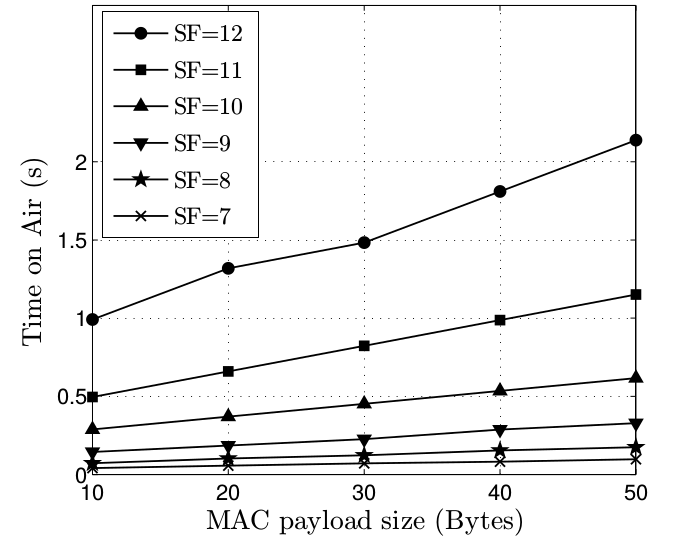
\includegraphics[scale=0.4]{images/estadoarte1.png}
\caption{Gráfica de tamaño de \textit{payload} MAC por tiempo que toma el paquete en llegar a destino. Fuente:\cite{Xavier}}
\label{arte:1}
\end{figure}
\begin{figure}[!ht]
\centering
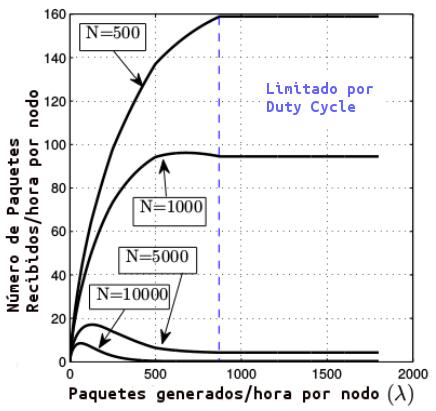
\includegraphics[scale=0.5]{images/estadoarte2.png}
\caption{Gráfica de paquetes generados en una hora por número de paquetes recibidos en una hora. Fuente:\cite{Xavier}}
\label{arte:2}
\end{figure}
Por otra parte, en otra investigación, se colocaron a prueba las capacidades de transmisión, pero en relación a la distancia máxima de transmisión, en zonas llanas sin interferencia por edificios o personas, y en zonas urbanas, con el objetivo de determinar si los LoRa cumplen con las especificaciones que entregan, y por otra parte, averiguar si pueden sobrepasar estas especificaciones técnicas entregadas por los fabricantes y descubrir nuevos límites para el uso de los dispositivos LoRa~\cite{Juha}.\\
En relación a las pruebas realizadas, el \textit{gateway} es situado a \SI{24}{\meter} sobre la altura del mar con una antena bi-cónica de \SI{2}{dbi} de ganancia, donde los nodos con los que se comunicará, uno estará navegando sobre un bote en un ambiente libre de edificios y árboles, mientras que el otro estará sobre el techo de un automóvil, donde cada nodo se alejará cada vez más sobre su medio de transporte, para evaluar si es posible transmitir efectivamente dentro de los parámetros que indican los fabricantes de LoRa, o si incluso es posible superar estas especificaciones. Los resultados obtenidos de las pruebas de medición de la investigación, pueden verse en las Tab~\ref{arte:3} y Tab~\ref{arte:4}~\cite{Juha}.\\
\begin{table}[!ht]
\centering
\begin{tabular}{|c|c|c|c|}
\hline
Rango & Número de            & Número de          & Porcentaje de  \\
      & paquetes trasmitidos & paquetes recibidos &  pérdida\\ 
      &                      &                    &   de paquetes \\ \hline
\si{0-2}{km} & \num{894} & \num{788} & \SI{12}{\percent} \\ \hline
\si{2-5}{km} & \num{1215} & \num{1030} & \SI{15}{\percent} \\ \hline
\si{5-10}{km} & \num{3898} & \num{2625} & \SI{33}{\percent} \\ \hline
\si{10-15}{km} & \num{932} & \num{238} & \SI{74}{\percent} \\ \hline
Total & \num{6813} & \num{4506} & \SI{34}{\percent} \\ \hline
\end{tabular}
\caption{Cantidad de paquetes transmitidos, recibidos y pérdida de paquetes por rango de distancia en medición hecha por nodo sobre auto. Fuente:\cite{Juha}}
\label{arte:3}
\end{table}

\begin{table}[!ht]
\centering
\begin{tabular}{|c|c|c|c|}
\hline
Rango & Número de            & Número de          & Porcentaje de  \\
      & paquetes trasmitidos & paquetes recibidos &  pérdida\\ 
      &                      &                    &   de paquetes \\ \hline
\si{5-15}{km} & \num{2998} & \num{2076} & \SI{31}{\percent} \\ \hline
\si{15-30}{km} & \num{690} & \num{430} & \SI{38}{\percent} \\ \hline
Total & \num{3688} & \num{2506} & \SI{32}{\percent} \\ \hline
\end{tabular}
\caption{Cantidad de paquetes transmitidos, recibidos y pérdida de paquetes por rango de distancia en medición hecha por nodo sobre bote. Fuente:\cite{Juha}}
\label{arte:4}
\end{table}
\newpage \noindent
Los resultados obtenidos a través de esta investigación, son de gran ayuda para el desarrollo de este proyecto, dado que entrega una guía de valores esperados al momento de realizar mediciones con los dispositivos reales~\cite{Juha}. Asimismo, otorga una guía de como se manifiestan parámetros como la tasa de errores en paquetes \gls{per}, para luego integrar al simulador con el fin de acercarlo más al funcionamiento real de los dispositivos. Y de la misma manera en la investigación que pone a prueba las capacidades de LoRa, entrega los conocimientos suficientes para poder modelar el comportamiento real de la saturación del canal en base a las retransmisiones de los nodos, y las colisiones generadas~\cite{Xavier}.
\section{Modelado de redes ALOHA}

El estándar \gls{lorawan} trabaja sobre la base del protocolo ALOHA, el cual es uno de los primeros protocolos de comunicación orientados a la conexión de dispositivos de forma inalámbrica. ALOHA trabaja sobre un canal de radio frecuencia, que utiliza tanto para el envío, como para la recepción de datos, por lo que para aumentar la transmisión efectiva de datos (\textit{throughput}), el protocolo ALOHA puro transmite datos en ventanas de tiempo aleatorias, y en caso de que el receptor no responda, en más del doble del tiempo que debiera responder con un acuse de recibo o \gls{ack}, el dispositivo emisor retransmitirá este paquete, y procederá con ese procedimiento hasta que reciba un acuse de recibo, con lo que concluye su transmisión de datos. Por otra parte Slotted ALOHA  o ``Ranurado'' implementa discretas ventanas de tiempo, donde el sólo podrá enviar o recibir datos, al inicio de una ventana de tiempo, con lo que se minimiza el número de colisiones~\cite{NORMAN}.\\
Slotted-ALOHA al ser un protocolo que permite las comunicaciones inalámbricas, con un buen manejo de colisiones, gracias a sus ventanas de tiempo discretas. Esta cualidad, llamó el interés de investigadores en generar ambientes virtuales, para simular el comportamiento de estos dispositivos, con el fin de poder realizar pruebas y estudios sobre el uso de este protocolo, sin necesidad de tener que instalar una red ALOHA con todos los costos asociados, tanto de tiempo como de dinero~\cite{Abdullah}.\\
En relación a los aportes del modelado de sistemas Slotted ALOHA, se realizan tres modelos que permiten el múltiple acceso de computadores mediante Slotted ALOHA, con el fin de otorgar modelos de simulación del protocolo para que estudiantes puedan comprender de mejor forma el cómo se comunican los dispositivos ALOHA~\cite{Abdullah}. Estos modelos de simulación imitan el comportamiento lógico del protocolo, entregando una herramienta útil para la comprensión del funcionamiento de redes de este tipo. Bajo este contexto, de la misma forma que nació la necesidad de modelar el funcionamiento del protocolo ALOHA. Adicionalmente se realizaron avances en el modelado de redes de sensores a gran escala, lo que entrega modelos que describen no sólo el funcionamiento del protocolo en condiciones ideales, si no que también la capacidad de modelar condiciones de borde y situaciones diferentes de las ideales, lo que acerca al módelo, a un comportamiento análogo al presente en los dispositivos reales~\cite{simulato}~\cite{simubook}.\\
Por otra parte, en una investigación se entrega un estudio sobre los diferentes simuladores de redes que existen, sus ventajas y desventajas frente al resto y los protocolos que acepta cada una de estas herramientas computacionales y sobre las capacidades de integración entre protocolos y tecnologías que ofrecen los distintos conjuntos de herramientas de simulación (\textit{frameworks})~\cite{Murat}.\\
En relación con este proyecto, todas las investigaciones mencionadas en este apartado, entregan la base teórica para el entendimiento del protocolo ALOHA, el cual es la base del funcionamiento de los dispositivos LoRa, y junto a esto hay investigaciones que entregan técnicas y métodos de cómo modelar tanto funcionamiento ideal y comportamiento lógico de protocolos en base a máquinas de estado ( en el caso de una simulación de eventos discretos), como también sobre el modelado de redes con parámetros como \gls{per}, atenuación de señal, entre otros elementos, que permiten el acercar un modelo de simulación, al comportamiento análogo de dispositivos reales~\cite{Abdullah}~\cite{simulato}. Cabe destacar que hay un artículo, que aporta con información sobre los diferentes \textit{frameworks} de simulación de redes, lo que permite tener una cantidad aceptable de información para poder decidir que software utilizar a la hora de desarrollar el simulador de dispositivos LoRa~\cite{Murat}.

\section{Integración de IoT en LoRaWAN}

%%tesis tomas, header compression y aplicaciones iot de lora%%
Los dispositivos LoRa, se comunican en base a transmisión de datos por radio frecuencia de un salto, esto junto con sistemas de modulación LoRa. En el escenario de enviar los datos obtenidos por los nodos LoRa con una aplicación web, el sistema no podría enviar los datos a través de Internet dado que no posee la capacidad de enrutamiento, no obstante el \textit{gateway} LoRa es capaz de realizar una retransmisión de los paquetes recibidos hacia un \textit{backend} (computador remoto) y con esto permitir la conectividad con aplicaciones web para la recepción de datos, aunque hasta el momento no es posible saber que nodo mandó un dato específico, o enviar datos desde el \textit{gateway} de forma directa hacia una dirección IP, esta carencia de los dispositivos LoRa limita las posibles aplicaciones con estos dispositivos. Bajo este contexto, algunos investigadores  han realizado modelos de compresión de cabeceras del protocolo IPv6 para dispositivos bajo el estándar \gls{lpwan}, donde se propone un modelo llamado 6LoWPAN que elimina ciertos campos de la cabecera del protocolo IPv6, de acuerdo a la configuración de los primeros \SI{16}{\bit}, con el fin de reducir el tamaño de la cabecera del paquete para direcciones IPv6 unicast, donde puede comprimirlos a \SI{512}{\bit} o \SI{128}{\bit} dependiendo de que campos se omiten, u omitir los campos opcionales por completo~\cite{lowpan}. En \cite{tomas}, este modelo teórico es aplicado a una red LoRa donde la cabecera IPv6 comprimida junto con el \textit{payload} deseado, se enviará a través del \textit{payload} de dispositivos \gls{lpwan} hacia el \textit{gateway}. Una vez llegado al \textit{gateway}, en este se construirá un paquete IPv6 con las especificaciones entregadas en la cabecera comprimida, donde adicionalmente se agregará la información relacionada al \textit{payload} del nodo emisor, y sus direcciones de red, las cuales al ser pertenecientes a una red LoRa, serán ingresadas en una tabla de enrutamiento que poseerá una equivalencia entre direcciones IPv6 y dirección de red LoRa, con el fin de poder luego enviar datos directamente desde los nodos hacia direcciones IPv6 y viceversa entregando la nueva función al \textit{gateway} LoRa de enrutador de mensajes.\newpage
\noindent
Cabe decir de que el \textit{gateway} LoRa para esta funcionalidad, necesita estar conectado al computador remoto que le provee de conexión a Internet, por medio de una interfaz virtual \gls{tun}, la que dejará pasar directamente los datos desde la red LoRa desde el \gls{tun} (donde está conectado el \textit{gateway} LoRa), hacia la salida a Internet del computador remoto. Si bien, la retransmisión de paquetes que posee nativa, realiza el mismo procedimiento, con la diferencia que ahora el \textit{gateway} LoRa creará el paquete de datos que se enviará, y este sólo será retransmitido hacia Internet, en cambio antes, el computador remoto tenía la labor de crear dicho paquete de datos, lo que entrega mayor autonomía e independencia de uso a los dispositivos LoRa.\\
Estos avances sobre la compresión de la cabecera IPv6 para dispositivos \gls{lpwan}, y la integración de IPv6 mediante el uso de estos modelos de compresión en una red LoRa, entregan a este proyecto el conocimiento necesario para poder diseñar un módulo que permita actuar de gestor de transición de una comunicación directa desde el \textit{gateway} hacia servicios locales dentro del computador remoto (sean bases de datos o aplicaciones web locales), y un intermediario mas seguro para la retransmisión de los paquetes, dado que al comunicarse directamente con la \gls{api} dentro del módulo bajo una conexión por \gls{socket}, entrega la posibilidad de realizar una conexión con un mayor nivel de seguridad, al tener la posibilidad de utilizar protocolos como TLS que dan la capacidad de cifrar la información y así evitar que un tercero atente contra la privacidad, integridad o disponibilidad de los datos.
\newpage
\section{Métodos de programación en C orientado a redes.}
%%libro de sockets, integracion de modulo%%
En muchas aplicaciones web, se han de utilizar scripts en sus servicios web para que realicen acciones deseadas por los desarrolladores, como también muchas veces son desarrollados scripts en el \textit{backend}, para realizar procedimientos como entrega de datos, creación de objetos, entre otros. El problema nace en que estos scripts son desarrollados en lenguajes como Python, Java o C, los que no tienen una orientación a red, si no, más bien a objetos, lo que dificulta el traspaso de datos obtenidos por los scripts hacia las aplicaciones web o sus servicios relacionados.\\
Bajo este contexto, nace la necesidad de que los scripts contenidos en aplicaciones web, se conecten tanto a \glspl{api} como a otros servicios existentes. Para poder llevar a cabo esta tarea, es necesario el uso de \glspl{socket}, los que constan de la apertura de conexiones bidireccionales a puertos determinados, que permiten la interacción en lectura como escritura contra servicios y aplicaciones web (Bases de datos, \glspl{api}, archivos de configuración, registros de depuración, etc). En el texto ``Programación en C orientada a redes'', enseñan múltiples técnicas, métodos y plantillas de código que permiten establecer conexión con servicios de red mediante el uso de \glspl{socket} en el lenguaje C~\cite{network}.\\
Los conocimientos aportados por este libro ayudaron en el desarrollo del módulo de transición de \gls{lorawan} a IPv6 en este proyecto, aportando métodos y funciones que otorgan la capacidad de conectar el \textit{gateway} LoRa con servicios y aplicaciones web. Esta conexión es generada en el mismo script que maneja la recepción de los mensajes de los nodos LoRa con el protocolo IPv6 integrado, resultando de esta forma, un sistema íntegro y con un nivel mayor de seguridad para poder conectar los datos obtenidos en la red LoRa con una aplicación web y todos sus servicios de red asociados.
\end{justify}
\justify
\begin{justify}
\chapter[Marco teórico]{Marco teórico}
\label{ch:marcoteorico}
En este capítulo se introducirán conceptos y problemas que serán abordados durante el desarrollo del proyecto, a través de la recopilación y análisis de información relacionada con el foco central de la investigación, además se explicará cada concepto clave relacionado al proyecto y luego se establecerá la relación de esta materia con el proyecto.

\section{ALOHAnet}
El sistema ALOHA, nació con el fin de crear un sistema que se adapte a aquellos escenarios donde las limitaciones de los diseños de redes computacionales implementados bajo conexiones cableadas no se adaptan a las condiciones a las que será expuesto, es decir, situaciones donde son preferibles las comunicaciones sobre la base de la radio frecuencia, por sobre las comunicaciones sobre las conexiones cableadas~\cite{NORMAN}.\\
La estructura de funcionamiento del sistema ALOHA, consta de un computador central conectado a un canal de comunicaciones por radio frecuencia, donde se poseerán dos bandas de un tamaño de \SI{100}{\kilo\hertz} en las bandas \SI{407.350}{\mega\hertz} y \SI{413.475}{\mega\hertz}, una de estas bandas estará destinada a la recepción de información desde los clientes al computador central, y la otra a el envío de información desde el computador central hacia los clientes, donde se genera un método de acceso aleatorio de multiplexación de un gran número de clientes de baja tasa de envío de datos hacia el computador central, donde la comunicación se lleva a cabo por un único canal de comunicaciones por radio~\cite{NORMAN}. Si bien los mensajes desde o hacia la computadora central no se pueden multiplexar, si se pueden utilizar técnicas como la multiplexación del canal y del tiempo, para dividir el canal de comunicaciones desde las consolas hacia la computadora central en un gran número de canales donde cada uno de los clientes usará una de estas subdivisiones del canal, esté activo o no, dado que si se otorgara tiempo de conexión exclusiva a una fracción del número total los clientes activos de la red, este esquema tendría las mismas deficiencias que el diseño de conexión cableada~\cite{Abdullah}.\\
Como puede apreciarse en la Fig~\ref{aloha:msg}, la estructura de los paquetes de datos que conformarán las trazas de datos en el protocolo ALOHA, constan de un tamaño de a lo más \SI{704}{\bit}, de los cuales pueden usarse \num{80} caracteres de \SI{8}{\bit} cada uno (un total máximo de \SI{640}{\bit} de \textit{payload}), \SI{32}{\bit} de control y paridad, más \SI{32}{\bit} de identificación. Estos paquetes están diseñados para transmitirse en un tiempo a lo más de \SI{29}{\milli\second} a una tasa de \SI{24000}{Bd} (número de símbolos/segundos)~\cite{NORMAN}.\\
\begin{figure}[!ht]
\centering
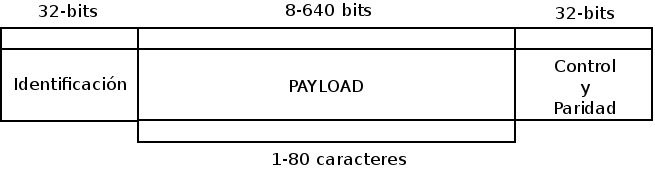
\includegraphics[scale=0.5]{images/alohamsg.png}
\caption{Formato de mensaje de protocolo ALOHA}
\label{aloha:msg}
\end{figure}\\
Con respecto al funcionamiento de este sistema ALOHA, este posee un tipo de conexión asíncrona donde los usuarios activos de una red con este sistema usarán un acceso aleatorio a la red, donde sólo se tomará en cuenta el tiempo donde se comienza el envío de los paquetes de datos y los canales disponibles para la transmisión (en base a la potencia del nodo y la disponibilidad del canal), dado que luego de esperar el doble del tiempo máximo de propagación, en el que  no recibe un paquete \gls{ack} que verifique la llegada del paquete enviado. El cliente retransmitirá este paquete periódicamente, hasta recibir un acuse de recibo por su contra parte. Para definir los límites de uso y capacidad del canal, se establece que el número máximo de clientes simultáneos en la red es de \num{324} clientes, dado que sobre dicho valor, la comunicación se vuelve inestable y con esto, el número promedio de retransmisiones se vuelve ilimitado por lo que satura el canal de comunicaciones~\cite{NORMAN}.\\
Este sistema es de vital importancia para este proyecto de título, dado que los dispositivos LoRa basan su comunicación en un sistema ALOHA puro (sistema descrito en esta sección), y ALOHA slotted o ``ALOHA \textit{con espacios}''. En la variante slotted del protocolo ALOHA, se agrega una comprobación de canal si está ocupado o no antes de transmitir, esta comprobación es llamada \gls{lbt}~\cite{Sornin}~\cite{Sornin2}. De esta manera se aumenta el \textit{throughput} por fracción de tiempo, por lo que es central el tener este sistema como antecedente, al desear imitar un comportamiento similar, conocer que destaca a LoRa por sobre ALOHA y para definir que variables se deben agregar a un modelo de ALOHAnet para que se comporte como LoRaWAN.
\section{Espectro expandido}
El acceso dinámico al espectro es una técnica que permite una optimización del uso de los espectros de frecuencia a usar para comunicaciones inalámbricas, donde se expande el espectro de la señal a utilizar para un determinado \textit{payload}, con el fin de blindar la señal generada por la frecuencia base, por este espectro expandido, lo que protege la señal contra interferencias externas de señales angostas, como también de intercepciones de la señal, dado que el receptor debe conocer la banda base para poder decodificar y demodular la señal de espectro expandido~\cite{modulation}.\\
\gls{sf} es el nombre utilizado por los desarrolladores de LoRa, para cada frecuencia base que se podrá utilizar como canal de comunicaciones entre los \textit{gateway} LoRa y los nodos. Los \gls{sf}, poseen la característica de que al necesitar un mayor alcance de transmisión, es posible sacrificar velocidad de transmisión (utilizando un canal definido para estos usos), por lo que el \gls{sf} con menor alcance (aproximadamente \SI{2}{\kilo\meter} de alcance), transmite a la mayor tasa de bits por segundo (aproximadamente \SI{5470}{bps})~\cite{orange}.\\
Adicionalmente los dispositivos LoRa analizan los espectros de frecuencia disponibles, donde luego para el caso particular de LoRa se usa la técnica \gls{lbt}, la que indica que en vez de probar una conexión y luego evaluar la condición del canal de radio, primero se debe censar y encontrar un canal disponible para de forma posterior iniciar la conexión con él~\cite{modulation}.
\section{Dispositivos LoRa}
Los dispositivos LoRa son artefactos para la comunicación inalámbrica de largo alcance, los que fueron diseñados con el fin de generar redes de dispositivos interconectados, que no requieren la intervención humana para funcionar, a este tipo de redes se les llama redes \gls{m2m}. Un ejemplo de este tipo de redes, son las redes que funcionan sobre la base de \gls{iot}, para así automatizar tareas de supervisión y censo de datos (usando sensores). Estos datos son distribuidos a través de una topología estrella hacia un \textit{gateway}, donde será el encargado de distribuir los datos hacia el microcomputador o servidor que realizará la conexión con la aplicación deseada.\\
El protocolo usado por estos dispositivos es LoRaWAN, el que permite al \textit{gateway} el transmitir configuraciones distribuidas (sincronización de reloj, uso de frecuencia definida, entre otras configuraciones), como también permite adaptar la tasa de envío y el delay de  la transmisión en pro de mejorar la comunicación con el/los nodos~\cite{Sornin}.\\
Los dispositivos clase B que utilizan este protocolo, poseen optimizaciones para una mayor duración de la batería de los nodos de la red, gracias a que mediante comandos MAC, ordena a los dispositivos a entrar en un modo reposo una vez realizada la subida de datos al servidor, donde el \textit{gateway} realiza una sincronización de relojes internos con el nodo, para luego calendarizar el próximo envío de datos~\cite{Sornin}.\\
Con respecto a la estructura del protocolo LoRaWAN, en este proyecto se centrará sobre el funcionamiento de la capa física (MAC) de LoRa. Esta capa posee tres clases principales dependiendo de la complejidad del dispositivo (clase A, B y C), las que definen la cantidad de funcionalidades presentes en el dispositivo.\\
Para el caso de los dispositivos bi-direccionales Clase A, poseen la funcionalidad mínima presente en todos los dispositivos Lora~\cite{Sornin2}. Estos dispositivos permiten la comunicación tanto de envío como de recibo de información, pero este espacio de transmisión depende de una pequeña variación aleatoria en el tiempo programado, lo que permite minimizar la cantidad de colisiones en la recepción de paquetes por parte del \textit{gateway} (protocolo tipo ALOHA)~\cite{Sornin}. Por otra parte, la obtención de datos desde el servidor a el nodo, debe esperar hasta la ventana de transmisión calendarizada, mientras que el nodo sólo requiere una ventana de bajada para sincronizar su configuración, después de haber transmitido hacia el servidor.\\
De la misma forma, los dispositivos bidireccionales de clase B, poseen la funcionalidad de los dispositivos A, y además poseen la capacidad de programar los envíos y recepciones de mensajes mediante el uso de espacios de recepción, estos espacios de recepción (o de conexiones entrantes) permiten una mayor capacidad de uso del canal dado que se realizan asignaciones dinámicas para evitar colisiones. Para esto el \textit{gateway} transmite una guía de sincronización (con los datos de su reloj interno) para así minimizar la posibilidad de colisiones de paquetes. Además los \textit{gateway} son capaces de adaptar entre la tasa de envío de datos y la sensibilidad de la transmisión, para mejorar la calidad del enlace a largas distancias de transmisión. Esta tasa adaptativa de envío de datos \gls{adr} es implementada en distintos canales que usan distintos espectros de frecuencia (\gls{sf}), lo que disminuye considerablemente las colisiones, dado que entre \gls{sf} no existen colisiones dado que los espectros de frecuencia poseen una banda banda base y una banda expandida, la banda expandida sirve de blindaje, lo que provee una protección contra interferencias de banda angosta. Por otra parte, la banda base permite el manejo multi-canal para las comunicaciones en LoRa, lo que entrega la capacidad de disminuir la saturación de los canales de comunicación, distribuyendo la utilización de los nodos y con esto disminuir la cantidad de colisiones en las comunicaciones.\\
Y en cuanto a los dispositivos de clase C , estos mantienen ventanas de transmisión casi continuas, ya que sólo las cierran al tener que transmitir. Estos dispositivos tienen un mayor consumo de energía en comparación con los dispositivos clase A y B, pero ofrecen la menor latencia en la comunicación servidor-nodo~\cite{Sornin}.\\
En cuanto al protocolo LoRaWAN, este posee una pila de 4 capas, las cuales son: La capa de aplicación, capa MAC, capa PHY y capa RF. Para este proyecto, se trabajará sobre la capa física o PHY ya que el objetivo de la simulación, es imitar el comportamiento físico de los dispositivos LoRa~\cite{Sornin2}.\\
Sobre la motivación por el estudio de los dispositivos LoRa, a causa de poseer una gran diversidad de usos~\cite{use1}~\cite{use2}, son de gran interés para el área de TI, considerando que permiten generar soluciones integrales de redes \gls{m2m}/\gls{iot} de forma inalámbrica y a bajo costo en comparación con otras soluciones. Además estos dispositivos tienen la capacidad de transmitir a largas distancias (\SI{2.5}{\kilo\meter} en zonas urbanas densas y \SI{15}{\kilo\meter} en zonas suburbanas), sin necesidad de una infraestructura costosa como es el caso de la tecnologías con una capacidad similar de transmisión como por ejemplo: GPRS, EDGE y LTE. No obstante aún no existen herramientas que permitan el diseño virtual de redes con estos dispositivos con el fin de: probar nuevos usos para esta tecnología, probar rendimientos esperados de una distribución específica, entre otros. Bajo este contexto, este proyecto pretende ser un aporte a la comunidad TI en el desarrollo de un modelo de simulación sobre la base del software de simulación de redes \OMNET, el que permitirá replicar el funcionamiento físico de los dispositivos LoRa (\textit{gateway} y nodos).
\subsection{Formato de mensaje LoRa}
Si se observa la Fig~\ref{fig:msg}, se puede ver que los mensajes en LoRaWAN poseen una estructura dividida en 4 capas de la misma forma que la pila del protocolo. La primera capa llamada Radio PHY Layer, tiene como objetivo el realizar la conexión de radio frecuencia entre los dispositivos que se disponen a transmitir datos. Por otra parte, la capa física está encargada de construir las tramas del mensaje con el fin de que, la capa de enlace transmita el \textit{payload} desde la capa MAC sobre el enlace de radio frecuencia. La capa física (PHY) usa bandas específicas de radio frecuencia dependiendo de la normativa de cada país\cite{Sornin}.\\
\begin{figure}[!ht]
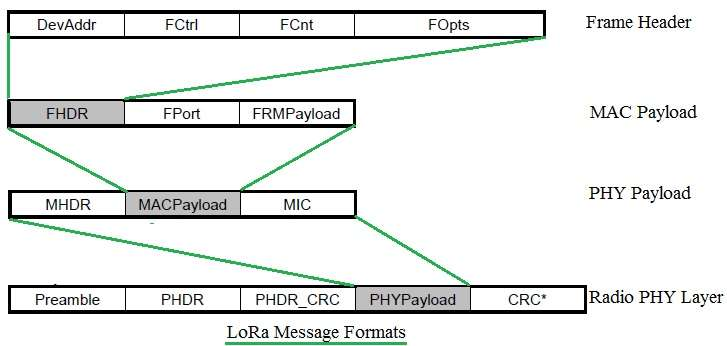
\includegraphics[scale=0.4]{images/LoRa-message-formats}
\caption{Formato de mensaje de protocolo LoRaWAN. Fuente:~\cite{Sornin}}
\label{fig:msg}
\end{figure}
\noindent
Para este proyecto se manipulará el modelo de simulación del protocolo ALOHAnet, con el fin de agregar parámetros de la capa física y de enlace que caracterizan al protocolo LoRa, y así poder imitar el comportamiento de los dispositivos LoRaWAN. Una vez identificados estos parámetros, se incluirán al modelo de simulación, para así tener la capacidad de replicar distribuciones y comportamientos esperados de los dispositivos físicos pero de manera virtual.\\
En cuanto al contenido de cada fragmento de los mensajes enviados por dispositivos LoRa, estos están definidos en las especificaciones técnicas del fabricante, los que son expuestos en la Tabla~\ref{tab:loramsg}~\cite{Sornin}.\\
Los indicadores a usar para el modelo de simulación planeado, son aquellos pertenecientes a la capa RF PHY, a la capa PHY \textit{payload} y la capa MAC \textit{payload}, sin contar tramas de capas superiores, dado que la herramienta de simulación trabaja en sobre la base de eventos, no analizando paquetes como lo haría un ``\textit{sniffer}'' de red, por lo que algunos campos de información contenida en la cabecera del mensaje es omitida dado este antecedente.
\begin{table}[!ht]
\begin{tabular}{|c|l|}
\hline
Campo de mensaje LoRa MAC & Descripción \\\hline
MHDR & Cabecera	MAC, longitud de un octeto\\\hline
MAC \textit{payload}	& Datos de capa superior\\\hline
MIC	Message Integrity Control & longitud de cuatro octetos\\\hline
FHDR  &	Cabecera de tramas de mensaje\\\hline
FPort	& Campo opcional de puerto de conexión\\\hline
FRMpayload	& Campo opcional de \textit{payload} \\&de tramas de mensaje\\\hline
Devaddr	& Dirección de dispositivo\\\hline
FCtrl & Octeto de control de tramas de mensaje\\\hline
FCnt &	Contador de tramas de mensaje,\\& longitud de dos octetos\\\hline
FOpts &	Opciones de trama, usadas para \\&ordenes de transporte\\ & en la capa MAC, longitud de \\&quince octetos\\\hline
\end{tabular}
\caption{Glosario de campos de mensajes LoRa}
\label{tab:loramsg}
\end{table}
En relación al formato del mensaje de LoRaWAN, a continuación se explican cada uno de los campos, y sus funciones dentro de los mensajes de LoRaWAN.\\
\begin{itemize}
\item MAC \textit{Header} (MHDR): Este campo contiene información cómo el tipo de mensaje (MType), donde se pueden tener mensajes como: join request, join accept, confirmed data up, entre otros. Este campo, también contiene la versión del formato de mensaje (Major), donde dependiendo de esta versión, el mensaje podría estar codificado o no. La estructura mencionada en este apartado, puede encontrarse en la Tab~\ref{msg:1}.

\begin{table}[!ht]
\centering
\begin{tabular}{|r|c|c|c|}
\hline
bit & 7..5 & 4..2 & 1..0 \\\hline
MHDR bit & MType & RFU & Major\\\hline
\end{tabular}
\caption{Formato de mensaje, campo cabecera MAC. Fuente:~\cite{Sornin}}
\label{msg:1}
\end{table}

\item MAC \textit{payload}: En este campo se encuentran las tramas de datos a enviar, dentro de este campo se encuentra información como la cabecera de la trama (\textit{Frame Header - FHDR}), seguido de dos campos opcionales, los cuales son \textit{Frame Port -FPort}, y \textit{frame payload- FRMpayload}. Estas campos contenidos en MAC \textit{payload}, serán explicados a continuación.
\begin{itemize}
\item \textit{Frame Header}: Este campo contiene la dirección del dispositivo (nodo) en el campo (DevAddr), un campo de control de trama (FCtrl), adicionalmente posee un contador de trama de mensaje (FCnt) y un campo llamado opciones de trama (FOpts) el cual tiene la función de enviar comandos MAC mediante este campo. Esta estructura puede apreciarse en la Tab~\ref{msg:2}.\\
\begin{itemize}
\item \textit{DevAddr}: Este campo posee la dirección en la red LoRa del dispositivo nodo al cual se le desea enviar la información.
\item \textit{Frame Control}: Aquí es contenida la información sobre el estatus del \gls{adr} (activo o no activo), el estado de llegada del paquete \gls{ack}, el largo del campo FOpts, y dependiendo si es un mensaje de bajada o subida, puede llevar un campo con la información de tramas pendientes (FPending), o tener un campo reservado para usos futuros (RFU) respectivamente.
\item \textit{Frame Counter}: En este campo se almacena el contador de tramas de mensaje, para tener un control sobre cuantos mensajes llegaron del total (en caso de ser paquetes fragmentados), y así pedir retransmisión de datos en caso de necesitarlo.
\item \textit{Frame Options}: Este campo almacena los comandos MAC a enviar, con un máximo de 15 octetos para enviar.
\end{itemize}

\begin{table}[!ht]
\centering
\begin{tabular}{|r|c|c|c|c|}
\hline
Tamaño (bit) & 32 & 8 & 16 & 0..120 \\\hline
FHDR & DevAddr & FCtrl & FCnt & FOpts\\\hline
\end{tabular}
\caption{Formato de mensaje, campo cabecera de trama. Fuente:~\cite{Sornin}}
\label{msg:2}
\end{table}

\item \textit{Frame Port}: Este campo opcional, entrega información del puerto destino, en el dispositivo receptor. En el caso de que el campo FRMpayload esté presente, el campo FpPort también debe estarlo. En el caso de poseer un valor 0 en el campo FPort, el campo FRMpayload, sólo enviará comandos MAC hacia su receptor. Y en el caso de que el valor de FPort, se encuentre entre \num{1}..\SI{223}{\bit}, FRMpayload contendría usos específicos para cada aplicación, mientras que los valores \num{224}..\SI{255}{\bit} en FPort, están reservados para usos futuros.
\item \textit{Frame payload}: En este campo es contenida la información a enviar al destinatario, la que puede variar desde comandos MAC estandarizados de LoRa hacia el receptor, o información específica de cada aplicación a usar con los dispositivos LoRa.
\end{itemize}
\item \textit{Message Integrity Control}: En el campo MIC, se almacena una especie de valor de \textit{hash} que permite comprobar la integridad del mensaje enviado. El valor almacenado en este campo, es calculado sobre todos los campos en el mensaje, y sobre la base del RFC4493.
\end{itemize}
\section{Diferencias entre LoRaWAN y ALOHAnet}
En relación a la diferencia entre LoRaWAN y ALOHAnet, esta radica en que el protocolo LoRa, si bien es implementado sobre la base del sistema ALOHA slotted, LoRaWAN es capaz mediante comandos MAC el colocar en modo reposo a los clientes que no necesiten mandar paquetes, y programar su próxima entrega de información, donde gracias a una sincronización de relojes entre el cliente y la puerta de enlace ( o concentrador LoRa), es posible generar un ahorro de consumo de energía considerable en los nodos, dando así una mayor autonomía a los dispositivos. Cabe destacar, de que ALOHAnet no es un protocolo de comunicación como lo es LoRaWAN, si no un sistema de comunicación inalámbrica para dispositivos, por lo que el tipo de mensajes que se utilicen en ALOHAnet, depende exclusivamente de que protocolo se utiliza sobre este sistema.\\
 En relación a las características de LoRaWAN, este posee una optimización de los usos de los canales de transmisión, ya que a diferencia de LoRa, ALOHA sólo usa una frecuencia para transmitir y otra para recibir información de sus clientes, por lo que si una puerta de enlace, llegaba a alcanzar un determinado número de clientes, las retransmisiones generadas por las colisiones de paquetes en el canal, generarían un colapso de la transmisión/recepción de paquetes denegando cualquier tipo de transmisión entre los actores de la red (Denegación de Servicio por saturación de canal). En cambio LoRaWAN usa la modulación de señal de espectro expandido, esta modulación expande a un mayor tamaño el espectro de la señal necesaria para transmitir un \textit{payload} determinado, esto genera un tipo de blindaje alrededor de la frecuencia base de la señal a interferencias externas de frecuencias angostas. Asimismo, si el receptor conoce la frecuencia base del mensaje enviado, es posible utilizar bandas de frecuencia dentro del espectro expandido, es decir otorga la capacidad de uso de multi-canales, y además mejora la seguridad de la comunicación en contra de intercepciones no deseadas, dado que si el receptor no conoce la frecuencia base, no le será posible filtrar mediante el uso de un filtro correcto de bandas, lo que resultaría en la obtención de sólo el ruido de la señal. Esta técnica de modulación, realiza una concesión de tasa de envío de datos a favor de un mayor alcance de transmisión y viceversa. Este proceso es realizado mediante el uso de canales con un ancho de banda corregido, con el fin de mejorar la comunicación entre nodo/\textit{gateway}, esto permite la optimización de la red a un ancho de banda constante, dado que al usar un espectro de señal expandido, es necesario pasar la señal por un filtro entre bandas o pasa bandas para obtener el contenido de la señal base y poder demodular el contenido sin alteraciones de ruido o interferencias ~\cite{modulation}.

\section{Simulación por eventos discretos}
Una simulación por eventos discretos es un tipo de modelado dinámico de sistemas que se caracteriza por mantener un estado global del sistema, que puede estar distribuido de forma lógica o física y que cambia de forma parcial dada la ocurrencia de un evento en particular. Cualquier estado en el sistema sólo cambia al ocurrir un evento definido previamente, donde uno o varios procesos que tienen por trabajo la ejecución de estos eventos. La ejecución de un evento en un sistema modelado por eventos discretos quita los eventos pendientes para el valor de tiempo actual y agregando unidades de tiempo establecidas en la definición de los parámetros y variables~\cite{simubook}.\\
Con respecto a los eventos, estos se definen como un suceso que realiza modificaciones a las variables de sistema. Todo evento es parte de una entidad u objeto de un sistema simulado, por lo que sólo cambiarán atributos de este, no interviniendo ninguna variable o atributo del resto del sistema~\cite{simubook}.\\
Referente a las entidades, estas se definen como los objetos o actores que en conjunto representan al sistema a simular. El estado global del sistema se conforma por el conjunto de estados de las entidades definidas.\\
En relación con el proyecto de título, se utilizará esta técnica de modelado, dado que se busca modelar el comportamiento físico de los dispositivos LoRa, el cual funciona en base a máquinas de estados o eventos. Este modelado tomará algunas variables como constantes o despreciables con el fin de simplificar el modelo de simulación, es decir, reducir el número de variables con el fin de centrar el foco del modelo de simulación, solamente en el funcionamiento lógico de la capa de enlace y física, junto con agregar parámetros reales existentes en las telecomunicaciones, tales como el porcentaje de pérdida de paquetes, entre otros.\\
Entre las variables a simplificar se encuentran ~\cite{orange}:\\
\begin{itemize}
\item Tasa de codificación (\textit{Code rate}).
\item El ancho de banda.
\item La tasa de envío de bits para cada \gls{sf}.
\item Los rangos de distancia que admite cada \gls{sf} .
\item El desfase de la señal de RF.
\item Tamaño del paquete a enviar.
\item Tiempo en aire del paquete.
\end{itemize}
No obstante, se realizarán mediciones con dispositivos reales, con los mismos valores fijados en los parámetros constantes, y con condiciones semejantes a las simuladas (i.e. atenuación de la señal equivalente a transmitir a una determinada distancia, entre otros.). Y de esta manera, asegurar un margen de error del modelo de simulación. Para determinar este margen de error, se compararán los valores obtenidos en la recepción y envío de paquetes entre los dispositivos reales con un cierto nivel de pérdidas y el modelo de simulación con características homologas. En el caso de que los resultados de las mediciones empíricas tengan sobre un \SI{3}{\percent} de diferencia con los datos del simulador, se realizarán los ajustes pertinentes para que se ajuste a la sensibilidad de error tolerada como válida (a lo más un \SI{3}{\percent}).
\section{Herramientas para simulación de redes}
Dentro de las herramientas de simulación por eventos discretos para redes sobre la base del protocolo ALOHAnet, se encontraron dos herramientas: NS-3 y \OMNET.\\
De estas herramientas se propone la utilización de \OMNET, dado que posee una interfaz gráfica muy amigable para la representación de los datos (representación de comunicación en la red, envío de mensajes, generación de gráficos, etc.), asimismo posee una interfaz de fácil uso para la manipulación de los archivos programables junto a un menú para ajustar variables de la simulación como el retardo de envío de mensajes, etc. Por otra parte, NS-3 si bien es un potente software de simulación, sus últimas versiones han tenido problemas de compilación en algunos módulos, inclusive en la integración del módulo MIXIM e INET al \textit{framework}, módulos que serán necesarios para el desarrollo del módulo de transición de LoRaWAN a IPv6. De la misma forma, se detectó de que NS-3 ha presentado en su última versión, intestabilidad en el desarrollo de simulaciones y problemas de integridad de datos~\cite{bugtrack}. Por estas razones, se ha preferido trabajar con el software \OMNET, el que en su última versión posee un número menor de incidencias sin resolver, en comparación con NS-3~\cite{bugtrack2}. Este antecedente, indica que las mediciones de \OMNET~tendrán mayor nivel de fiabilidad, que un programa que posee un mayor número de errores sin resolver.

\end{justify}
\justify
\begin{justify}
\chapter[Resultados]{Resultados}
\label{ch:resul}
En este capítulo, se presentarán los aportes en el desarrollo del modelo de simulación, como también en el módulo de transición entre IPv6/LoRaWAN. Adicionalmente se entregarán los resultados obtenidos de las mediciones realizadas en la transmisión de nodos LoRa tanto en el ambiente virtual como en el empírico, esto acompañado de el análisis de los resultados, de las anomalías presentes, de los obstáculos que se presentaron en el desarrollo de estas pruebas y como ésto afectó a los resultados.

\section{Definición de variables y parámetros}
\label{sec:param}
Para el desarrollo del modelo de simulación es necesario acotar el sistema a simular, a los objetivos centrales del proyecto, para así evitar perder el foco deseado por realizar un modelo complejo, es decir, evitar realizar un modelo que incluya de forma innecesaria, variables que no generan un impacto tal en las mediciones, que merme la sensibilidad del modelo de simulación por sobre el nivel tolerado (\SI{3}{\percent}). Dado que el fin de esta simulación es imitar el comportamiento físico de los dispositivos LoRa, algunos datos que en condiciones reales son variables serán tomadas como parámetros estáticos con el fin de simplificar el modelo de simulación. Los valores asignados a estas variables, fueron obtenidos en la guía del desarrollador para dispositivos LoRa de la empresa Orange~\cite{orange}. Estos datos son escogidos dado que múltiples investigadores al realizar pruebas empíricas, usaron estos mismos datos como base para sus investigaciones con los dispositivos LoRa, obteniendo resultados muy cercanos a los que entrega la especificación de LoRa~\cite{Juha}. Los parámetros constantes de este sistema a modelar son los siguientes:
\begin{itemize}
\item Tasa de codificación=$\frac{4}{5}$
\item Ancho de Banda=\SI{125}{\kilo\hertz}
\item \gls{per}=\SI{1}{\percent}
\item Tasa de envío de datos en \textit{gateway} inicial=\SI{300}{bps}
\label{para:1}
\end{itemize}
\noindent
En relación a los parámetros fijos para el modelo de simulación, se aprecia en Tab~\ref{tab:par}, que se han definido valores fijos para variables dependientes de los \gls{sf} (tasa de envío de datos, alcance de transmisión, \textit{Time on Air}) a usar en la etapa de \gls{adr} de la comunicación LoRa~\cite{orange}.
\begin{table}[!ht]
\centering
\begin{tabular}{|c|c|c|c|}
\hline
\gls{sf} & bit rate & Alcance de Transmisión & \textit{Time on Air}\\ \hline
SF7 & $5470bps$ & $2km$ & $56ms$ \\ \hline
SF8 & $3126bps$ & $4km$ & $100ms$ \\ \hline
SF9 & $1760bps$ & $6km$ & $200ms$ \\ \hline
SF10 & $980bps$ & $8km$ & $370ms$ \\ \hline
SF11 & $440bps$ & $11km$ & $740ms$ \\ \hline
SF12 & $290bps$ & $14km$ & $1400ms$ \\ 
\hline
\end{tabular}
\caption{Asignación de valores para los diferentes \glsentryname{sf}.}
\label{tab:par}
\end{table}
\subsection{Arquitectura de red}
Para la comunicación en una red LoRa, se requiere una cantidad mínima de componentes para lograr la comunicación efectiva entre los dispositivos. Estos componentes mínimos para la comunicación son los siguientes:\\
\begin{itemize}
\item Concentrador LoRa (\textit{gateway})
\item Nodo LoRa
\item Micro computador conectado a Concentrador (\textit{backend})
\item Micro computador conectado a Nodo (\textit{backend})
\end{itemize}
Esta distribución mínima de componentes para asegurar la comunicación, puede verse en la Fig~\ref{lora:arc}. Esta arquitectura de red mínima se debe a que los dispositivos LoRa, sólo son provistos de las placas y antenas para el envío y recepción de paquetes en una red LoRa, pero no poseen la inteligencia para tomar decisiones o realizar acciones de forma autónoma, por lo que se requieren micro computadores (podría ser cualquier tipo de computador, pero se sugiere micro, para ahorrar consumo de energía) que le otorgue la inteligencia y sustente en energía a los dispositivos LoRa y a los sensores conectados a éstos. Adicionalmente, puede proveerse de un servidor que aloje una \gls{api} y una base de datos, con el fin de intercomunicar un servicio web, o para almacenar los datos censados en la red LoRa.\\
Para las pruebas realizadas en las mediciones de ambientes reales, se utilizó el esquema de arquitectura de red mínima, dado que al modelar los resultados obtenidos, tanto del funcionamiento lógico, como del funcionamiento físico, es posible proyectar estos resultados en arquitecturas de red a redes con un nivel mayor de complejidad, es decir, con un mayor número de elementos o distribuciones de éstos. Bajo este contexto, se realizaron pruebas representativas tanto para esta arquitectura mínima, como para un mayor número de nodos, gracias a la proyección que entrega el modelo de simulación.
\begin{figure}[!ht]
\centering
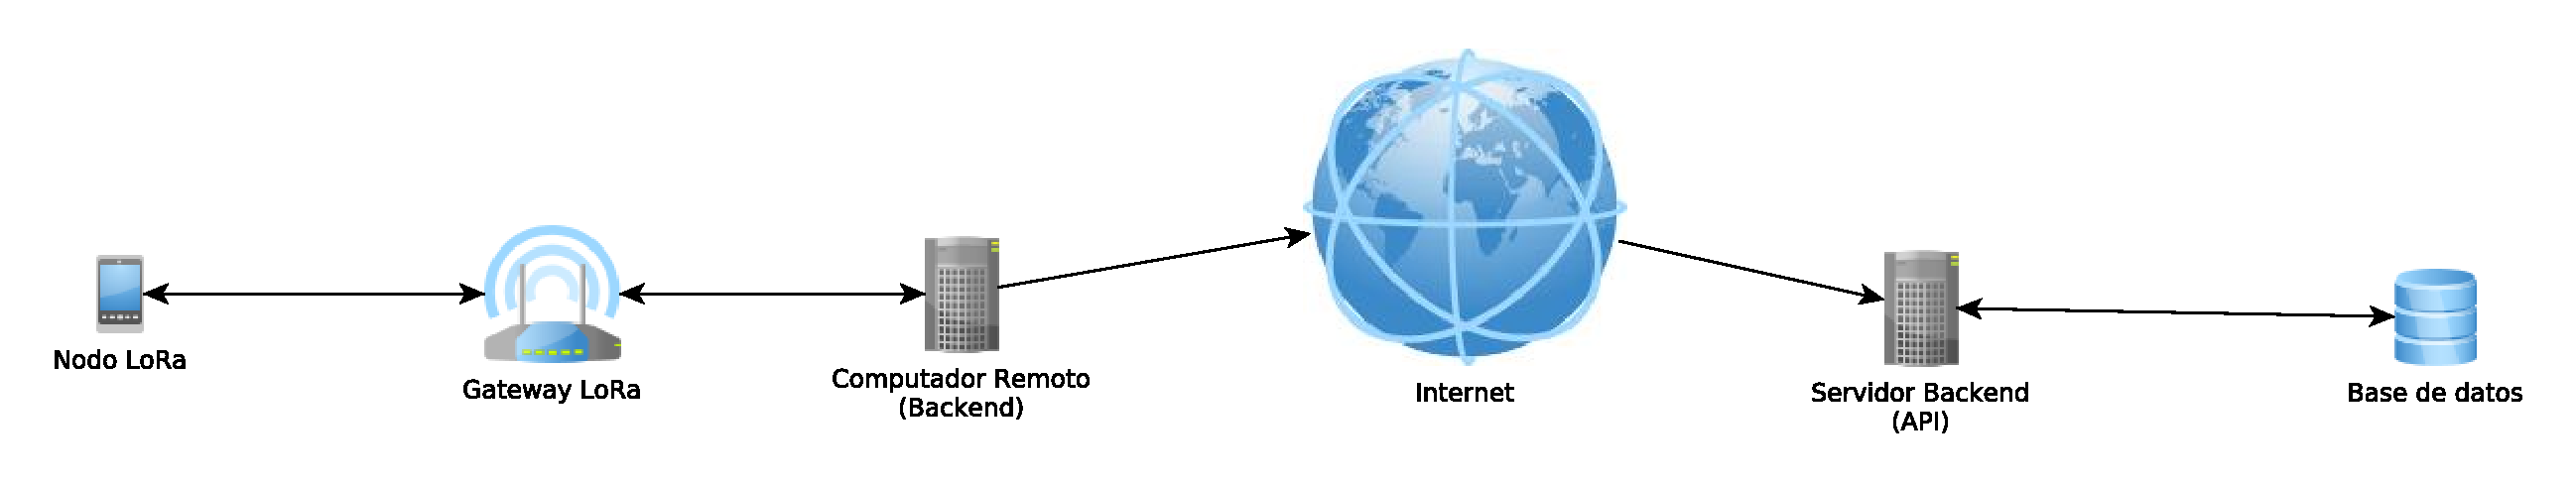
\includegraphics[scale=0.45]{diagramas/redminimalora.eps}
\caption{Diagrama de arquitectura de red mínima para una red LoRa}
\label{lora:arc}
\end{figure}
\newpage
\noindent
\section{Definición de fases de transmisión en LoraWAN}
Para que exista comunicación entre los nodos y \textit{gateway} LoRa deben ejecutar fases de comunicación, las que dan inicio a eventos, cómo el envío de un mensaje o el cambio de estado de un dispositivo. El identificar estas fases, para luego modelarlas, generará que el modelo de simulación sea más apegado al funcionamiento real de los dispositivos a simular. Dentro de las fases identificadas en la comunicación de los dispositivos LoRa se encuentran los siguientes:
\begin{itemize}
\item Fase de Emparejamiento
\item Fase de Transmisión
\begin{itemize}
\item[$\diamond$] Fase de Retransmisión (en caso de existir colisiones)
\end{itemize}
\item Fase de Reposo
\end{itemize}

\subsection{Fase de emparejamiento}
Durante esta fase, el nodo enviará un paquete \textit{Join Request} a todos los \textit{gateway} disponibles. Una vez que el \textit{gateway} reciba este mensaje, deberá responder dos mensaje de bajada que contendrán los identificadores de red, y dirección de la red LoRa para el nodo, adicionalmente se agregarán las llaves de sesión y aplicación en caso de que estén creadas.\\
Dado que en este modelo de simulación se busca sólo la simulación del comportamiento físico, los mensajes a programar en el modelo de simulación no poseen contenido alguno más que el nombre del mensaje que se está enviando, esto fue diseñado así para tener un mayor control en la depuración de la simulación y además para entregar un disparador de eventos de un objeto simulado al otro (nodo a \textit{gateway} y viceversa).\\
Los mensajes de bajada tendrán un desfase de envío de \SI{20}{\micro\s} más el tiempo que demora el paquete en llegar a destino, estos mensajes se identifican como \textit{Downlink-1} y \textit{Downlink-2}. \newpage \noindent 
Una vez que el nodo reciba estos mensajes, enviará dos mensaje \gls{ack}, pero luego de recibir los dos mensaje de bajada. En esta etapa, es donde internamente el nodo asigna todas las variables recibidas desde el \textit{gateway} para su correcto funcionamiento en la red.\\
Cuando el nodo envíe ambos mensajes de confirmación de los mensajes \textit{Downlink-1} y \textit{Downlink-2}, se asigna una variable distintiva (identificador de red y dirección de red LoRa) para evitar que un envío de datos sea rechazado por el \textit{gateway}, dado que en la simulación los mensajes no tendrán contenido, se asigna una variable tipo bandera, para distinguir a los nodos emparejados de los que no. Este fenómeno puede visualizarse en la Fig~\ref{pair:1}~\cite{Sornin}.
\begin{figure}[!ht]
\centering
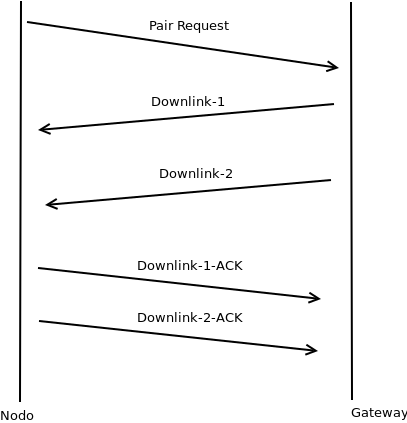
\includegraphics[scale=0.5]{diagramas/pair}
\caption{Diagrama de flujo de mensajes para fase de emparejamiento en red LoRa}
\label{pair:1}
\end{figure}
\newpage
\noindent
\clearpage
\subsection{Fase de transmisión}

En el caso de que el nodo reciba bien ambos mensajes de bajada, como se observa en la Fig~\ref{trans:1}, se enviará un mensaje de petición de envío de datos (\textit{Uplink request}), a lo que en condiciones ideales (sin colisiones ni saturación de canal), el \textit{gateway} deberá responder con una confirmación de la petición de envío, deteniendo cualquier transmisión por aquel canal y quedando a la espera de la recepción del mensaje proveniente del nodo. El nodo una vez que recibe el paquete \gls{ack} de la petición de envío , este envía el paquete de datos al \textit{gateway}, donde en caso de no haber colisión, el \textit{gateway} respondería nuevamente con un paquete \gls{ack}, terminando con esto la fase de transmisión.\\


\begin{figure}[!ht]
\centering
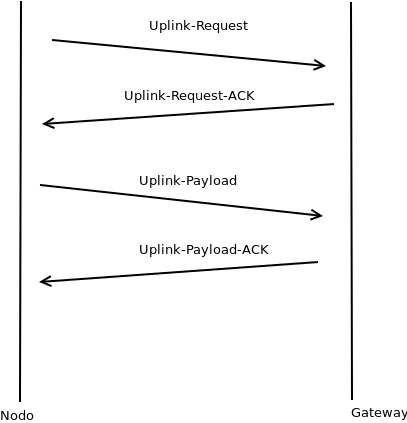
\includegraphics[scale=0.6]{diagramas/transmit}
\caption{Diagrama de flujo de mensajes en fase de transmisión de paquetes en red LoRa}
\label{trans:1}
\end{figure}
\newpage
\subsubsection{Fase de retransmisión}
\justify
En el caso de que en cualquier fase ocurra una colisión o una interferencia que corrompa un bit en un paquete, el paquete será descartado y no llegará a destino, por lo que todos los dispositivos LoRa poseen un indicador de tiempo agotado (\textit{Timeout}) el que es igual a:
 
\begin{eqnarray}
 \textit{Timeout} [\SI{}{\milli\s}]= 2(\textit{Time on Air}) [\SI{}{\milli\s}]\end{eqnarray} \\
, donde \begin{eqnarray}
 \textit{Time on Air} [\SI{}{\milli\s}]= \frac{\textit{Largo del Paquete} }{\textit{Tx Data Rate}} \frac{[\SI{}{\bit}]}{[\SI{}{bps}]}\end{eqnarray}
\noindent
En la Fig~\ref{retrans:1} se describe el proceso lógico que realiza el simulador en caso de no recibir un paquete \gls{ack} luego de la petición de conexión, en el caso que el tiempo transcurrido sea mayor al valor de la variable \textit{Timeout}, el nodo volverá al estado previo de envío dependiendo si está pareado o no. En el caso de que se encuentre emparejado, volverá a la fase de transmisión para transmitir nuevamente el paquete \textit{Uplink-request} hasta que el \textit{gateway} le responda. Si el nodo no está emparejado, este volverá a la fase de emparejamiento donde enviará el paquete \textit{Pair-request}, hasta que el \textit{gateway} le responda con las dos ventanas de bajada (\textit{Downlink-1} y \textit{Downlink-2}).
\begin{figure}[!ht]
\centering
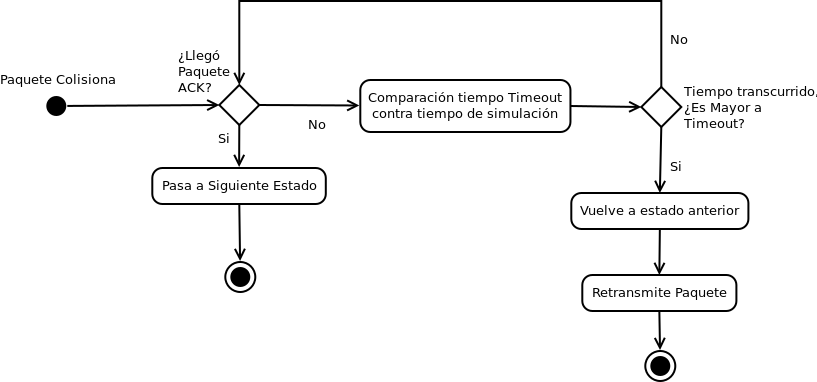
\includegraphics[scale=0.4]{diagramas/retrans}
\caption{Diagrama de estados que representa la fase de retransmisión}
\label{retrans:1}
\end{figure}
\subsection{Fase de reposo}
Luego de la transmisión del paquete \textit{Uplink-payload} desde el nodo al \textit{gateway}, si el \textit{gateway} contesta nuevamente con un último paquete de confirmación \gls{ack}, en este paquete el \textit{gateway} enviará los datos de su reloj interno para sincronizar y programar el próximo envío de datos, a lo que el nodo sincroniza su reloj interno y entra en un estado de reposo, a lo que no transmite ni recibe nada hasta que se cumpla la condición entregada por el \textit{gateway}. Este tiempo de reposo, es configurable desde el \textit{gateway}, con el comando MAC DutyCycleReq~\cite{Sornin}.
\subsection{Pérdida de paquetes}
Con el fin de acercar más a la realidad el modelo de simulación, se programó una función que simula la pérdida de paquetes en los distintos \gls{sf}, ésto lo realiza llevando una contabilidad de los mensajes recibidos, y genera una comparativa con el porcentaje de pérdida en la recepción donde se tienen tres condiciones principales. La primera es que el porcentaje de pérdida sea mayor que cero, y ésta debe ser siempre verdadera, dado que si fuera cero no debería entrar a la función que desechará paquetes. La segunda condición es una condición compuesta, donde debe cumplirse que el coeficiente entre el contador de recepciones con error, por el contador de envíos recibidos correctamente multiplicado por cien debe ser menor que el porcentaje de pérdida de paquetes, o en cambio es posible de que se cumpla de que el contador de errores sea igual a cero, con lo que también entraría a la función que desechará la recepción de datos.\\
Con esta función es posible emular un ambiente mas cercano al real, al poder incluir condiciones desfavorables en la simulación, como las que son posibles de encontrar en la vida real.

\section{Módulo de transición LoRaWAN/IPv6}
Para el desarrollo del módulo de transición de LoRaWAN a IPV6 se modificó el programa desarrollado por SemTech~\cite{script} para comunicar el \textit{gateway} con el nodo, generando un tipo de \textit{Middleware} entre la red LoRa y las redes externas a esta.\newpage \noindent
Gracias a modificaciones realizadas al script de SemTech, ahora es posible la obtención y visualización del \textit{payload} de forma íntegra y su retransmisión hacia redes externas a la red LoRa~\cite{tomas}.\\
En cuanto a llevar a cabo la retransmisión hacia redes externas de los paquetes LoRaWAN, hace falta generar una conexión puente que comparta salida a Internet al \textit{gateway} LoRa, esto se logra a través del uso de iptables u otro gestor de reglas de conexiones entrantes y salientes. Y luego mediante el uso de \glspl{socket} en C realizar la conexión hacia una base de datos o aplicación web, para luego procesar dichos datos y finalmente ser mostrados en algún front-end o servicio web.
\subsection{Funcionamiento}
El funcionamiento de este módulo es el siguiente, una vez que el \textit{gateway} ya posee la capacidad de escuchar, se debe lanzar un ping en IPv6 desde la Raspberry que posee de back-end. Una vez realizado esto comenzará una transmisión de paquetes donde se capturará el \textit{payload} del mensaje de LoRaWAN y se mostrará por pantalla,  ``Manda'' y ``LLega'' dependiendo si el mensaje llega de forma íntegra o no al \textit{gateway} (la cantidad de bytes especificada en la configuración, debe ser la misma cantidad de bytes que los contenidos en el struct array), en dicha parte del código se implementó un \gls{socket} en C para comunicarse con una base de datos MySQL creada para la interacción con este módulo, dado que si es posible comunicarse con la base de datos y realizar consultas a la base de datos (insert-delete-update) será posible la comunicación con casi cualquier servicio web que admita conexiones desde clientes.\\
En el extracto de código~\ref{anexc:1}, se presenta el código que maneja los métodos que permiten enviar datos como la IP del \textit{gateway} (obtenida mediante la implementación de IPv6 sobre LoRaWAN~\cite{tomas}), junto con el \textit{payload} a una base de datos, que en este caso sería una base de datos local. De esta forma se puede visualizar cómo es posible generar una capa intermedia de comunicaciones para el envío de datos entre la red LoRa y un servicio web deseado.
\subsection{Contribuciones}
Gracias a la contribución de la implementación de IPv6 en LoRaWAN, y a los mensajes de depuración del script para que imprima por pantalla los estados de los mensajes tanto salientes como entrantes (sólo los que llegan íntegros), es posible extraer el \textit{payload} de los mensajes enviados por los nodos hacia el \textit{gateway} para luego poder enviarlo hacia afuera para su almacenamiento en una base de datos, o para análisis de los datos en alguna aplicación sea web o móvil. Esto da la capacidad a una red LoRa de ejecutar comandos MAC, como también el extraer los datos hacia una aplicación que analice y cense los datos obtenidos, entre otros posibles usos~\cite{tomas}.
\subsection{Consideraciones}
Dados los problemas de conectividad presentes en los dispositivos físicos que se utilizaron durante la ejecución de las pruebas, tanto en el desarrollo del módulo como en las pruebas  de verificación, estas pudieron ser llevadas a cabo bajo la condición de poseer ambos dispositivos (Nodo y \textit{gateway}), a distancias muy cortas para maximizar la conectividad, dado que el objetivo de este módulo es probar la posibilidad de extraer datos de una red LoRa hacia Internet, y no el probar la capacidad de transmisión de los dispositivos físicos. Esto es mencionado dado que muchas veces los paquetes no llegan desde el nodo al \textit{gateway}, y no porque este no haya sido enviado, si no porque el \textit{gateway} lo detecta como mensaje, al analizar el campo MIC del paquete recibido, donde en el caso de que el \textit{hash} no coincida con el válido, se toma como paquete corrupto. Por lo que este módulo en esos casos no es capaz de enviar nada.
%%%PRUEBAS%%%%
\section{Parámetros y variables de mediciones}
Para verificar el funcionamiento del modelo de simulación de los dispositivos LoRa, se establecieron ciertos parámetros a medir, los que serán a posterior indicadores del buen o mal funcionamiento del modelo de simulación. Estos parámetros son, los cambios de estado de los dispositivos LoRa (en el caso del simulador), para verificar que está realizando todo el proceso de forma correcta. Además, se medirá el número de colisiones contra la cantidad de mensajes enviados y erróneos, para calcular el porcentaje de pérdida de paquetes estimado en cada prueba de transmisión. Estas pruebas se realizarán primero en el ambiente real, con el fin de obtener un valor estimado del porcentaje de pérdida de paquetes real, el que luego se aplicará al modelo simulado y será contrastado tanto entre el ambiente real, el ambiente virtual, como también contra los porcentajes de pérdida de paquetes obtenido investigaciones relacionadas~\cite{Juha}. Este contraste de resultados, es realizado ya que el modelo de simulación, es desarrollado en un principio en una condición ideal de transmisión, por lo que no es afectado por ninguna variable del ambiente (interferencia por otras señales, edificios, interferencia por fuentes de poder,etc.) lo que lo hace poco real y por tanto no fiable como modelo de simulación, por lo que el objeto de este contraste es volver más fiable el modelo, agregando condiciones presentes en la realidad, al canal de transmisión virtual.\\
Adicionalmente para las pruebas de simulación se dispuso una distribución específica de los nodos para cada canal o \gls{sf}, dicha distribución es posible de encontrar en la Tab~\ref{tab:prueba}, donde se mostrará que cantidad de nodos está asignado a cada \gls{sf}, y que distancia en metros se le asignó para temas de la simulación. Estos datos explican la distribución de hasta diez nodos, la cual para las pruebas de cien nodos fue repetida diez veces con el fin de mantener la misma distribución pareja de nodos. Cabe decir que la correspondencia entre la distancia desde los nodos hasta el \textit{gateway} con el \gls{sf} asignado, fue tomado de datos de los desarrolladores de LoRa~\cite{orange}.\\
En relación a las pruebas de cambio de estado, en la Tab~\ref{tab:estados} se muestran la correspondencia de cada valor numérico con cada estado de los nodos durante la simulación. Dentro de los estados disponibles para los nodos se encuentran los siguientes:
\begin{itemize}
\item IDLE: Este estado es el inicial para cada nodo en la red, es el encargado de enviar el \textit{Pair request} al \textit{gateway} y luego quedarse a la espera de recibir las dos ventanas de descarga desde el \textit{gateway}.
\item PRERECEIVE: Este estado, sólo se encarga de esperar hasta que el \textit{gateway} envíe ambas ventanas de descarga, donde al llegar éstas y si el nodo no esta emparejado, envía la orden de cambiar a estado TRANSMIT.
\item TRANSMIT: Este estado es activado al recibir las ventanas de descarga. Es el estado que genera los mensajes \textit{Downlink-1-ack} y \textit{Downlink-2-ack}, los que serán enviados al \textit{gateway} para certificar de que se recibió la información de estos paquetes, los que en el caso de un emparejamiento real tendría relación con los identificadores de red, identificadores de aplicación y los tiempos que debe esperar entre cada ventana de subida de información.
\item RECEIVE: En este estado, se envía el primer \gls{ack} correspondiente a la primera ventana de descarga. Este estado, da paso directo al estado RECEIVE2, dado que la diferencia de recepción de envío de la primera y segunda ventana, es poca en comparación con el resto de mensajes (más o menos \SI{20}{\micro\s}, ésto permite la correcta recepción de ambos mensajes, sin pérdida del primero, o falla de sincronización en la fase de emparejamiento por un sobre encolado de mensajes.
\item RECEIVE2 : En este estado, se envía el segundo paquete \gls{ack} correspondiente a la segunda ventana de descarga. Este estado da paso directo al estado IDLE2 , con el fin de cumplir la ventana de tiempo antes de enviar información hacia el \textit{gateway} y no colisionar con otro envío de información.
\item IDLE2: Éste es el encargado de enviar la petición de subida de información al \textit{gateway}, con el fin de evitar pérdida de datos de medición en caso de que el \textit{gateway} no esté disponible para el recibimiento de esta información. Este estado da el paso al estado \gls{ack}, para poder recibir el primer mensaje \gls{ack} correspondiente a esta petición.
\item \gls{ack}: Este estado se activa, sólo si es recibido el mensaje \gls{ack} correspondiente a la petición de envío de información y si el estado anterior fue IDLE2. Si es recibido este mensaje, el nodo envía el \textit{payload} correspondiente a la información de medición que posee en ese instante al \textit{gateway} y queda a la espera de el paquete \textit{ack-payload-2}. Este estado da paso al estado SLEEP.
\item ACK2: Este estado fue creado con el fin inicial de depurar la interacción entre \textit{gateway} y nodos, por lo que para las pruebas y el uso actual del simulador, no posee un uso funcional. Actualmente se reserva para usos futuros.
\item SLEEP: Este estado se activa luego de recibir el paquete \textit{ack-payload-2} correspondiente a el \textit{payload} enviado desde el nodo al \textit{gateway}, donde luego se colocará al nodo en estado de reposo hasta la siguiente ventana de envío. Una vez cumplido el tiempo de espera del nodo, éste volverá al estado IDLE2 para volver al ciclo de envío de datos. Luego de este estado, no se vuelve al estado de emparejamiento, dado que sólo es necesario emparejar una vez con el \textit{gateway} de la red, a menos que se posea una topología estrella de estrellas que requiera otro tipo de interacción, el cual no es abarcado por este proyecto.
\end{itemize}

\begin{table}[!ht]
\centering
\begin{tabular}{|c|c|c|}
\hline
Número de Host & \gls{sf} & Distancia a \textit{gateway} [Metros]\\ 
\hline
1 & 7 & 1 \\
\hline
2 & 7 & 2 \\
\hline
3 & 8 & 3 \\
\hline
4 & 8 & 4 \\
\hline
5 & 9 & 5 \\
\hline
6 & 9 & 6 \\
\hline
7 & 10 & 7 \\
\hline
8 & 11 & 11 \\
\hline
9 & 12 & 14 \\
\hline
10 & 12 & 14 \\
\hline
\end{tabular}
\caption{Tabla con distribución de nodos en cada \glsentryname{sf} para pruebas de simulación}
\label{tab:prueba}
\end{table}

\begin{table}[!ht]
\centering
\begin{tabular}{|c|c|c|}
\hline
Indicador de estado & Estado de nodo\\ 
\hline
0& IDLE \\
\hline
1& TRANSMIT \\
\hline
2& PRERECEIVE\\
\hline
3& RECEIVE\\
\hline
4& RECEIVE2\\
\hline
5& IDLE2\\
\hline
6& ACK\\
\hline
7& ACK2\\
\hline
8& SLEEP\\
\hline

\end{tabular}
\caption{Tabla con relación de indicador de estado y la etapa alcanzada por cada nodo en la simulación}
\label{tab:estados}
\end{table}

\subsection{Pruebas realizadas}
Las pruebas realizadas constan de dos tipos, la que comprueba los cambios de estado de los nodos para verificar el correcto funcionamiento de la lógica de los dispositivos LoRa aplicados en el modelo de simulación dependiendo de la cantidad de nodos, y para verificar la demora del emparejamiento en casos de mayor saturación del canal, y las prueba de transmisión donde tanto los dispositivos reales como los virtuales, tendrán las mismas configuraciones iniciales, y donde se obtendrá el porcentaje de pérdida de paquetes, dato con el que se podrá establecer que porcentaje de sensibilidad posee el modelo de simulación y con esto validarlo, o establecer un ajuste, para alcanzar el nivel de sensibilidad esperado. Asimismo se generaron pruebas de transmisión en el simulador con 1, 10 y 100 nodos, con el fin de determinar el crecimiento del número de colisiones que generan por canal (\gls{sf}) los nodos, y de la misma forma para determinar la sensibilidad alcanzada en la simulación de pérdidas de paquetes agregada al modelo de simulación.

\section{Análisis de resultados}
En esta sección, se presentarán las observaciones y estudios sobre los resultados obtenidos, en las pruebas realizadas en este proyecto. Las pruebas realizadas se separan en dos ambientes:
\begin{itemize}
\item Ambiente real: Dentro de las pruebas en el ambiente empírico, se realizaron mediciones de conectividad entre dispositivos reales (nodo/\textit{gateway}), para poder determinar como se comportan los dispositivos en una comunicación normal. Y adicionalmente para tener en cuenta, como modelar la pérdida de paquetes por corrupción de datos.
\item Ambiente virtual: En este ambiente se realizaron dos tipos de pruebas. La primera prueba fue examinar los cambios de estado con diferentes niveles de utilización de canal (i.e. ideal, saturación baja y saturación alta), con el fin de averiguar si el comportamiento lógico, estaba siendo simulado de forma correcta.\\
La segunda prueba fue el realizar una medición, sobre las colisiones y los paquetes con error en las diferentes distribuciones de nodos (1, 10 y 100 nodos). Esta prueba tuvo el fin de comprobar si el modelamiento de los paquetes con errores fue exitoso, y de la misma manera, determinar si el modelo de simulación, seguía teniendo matices de LoRaWAN. 
\end{itemize}

\subsection{Cambios de estado}
Se realizaron tres instancias de esta prueba, cómo puede verse en la Fig~\ref{prueba:1}, la primera con un número menor a la cantidad de \gls{sf} disponibles, con el fin de corroborar la correcta transición de estados en una transmisión ideal, es decir, sin colisiones ni pérdidas de paquetes. La segunda instancia puede verse en la Fig~\ref{prueba:2} , donde se realizó la misma prueba pero ahora con diez nodos, con el fin de ver como responde frente a las colisiones y retransmisiones al aumentar la saturación del canal. Finalmente en la tercera instancia presentada en la Fig~\ref{prueba:3}, se muestra el nivel de retardo en la transición de estados, al aumentar el número de nodos a 100, manteniendo la proporción de la distribución definida en la Tab~\ref{tab:prueba}.\\
\begin{figure}[!b]
\centering
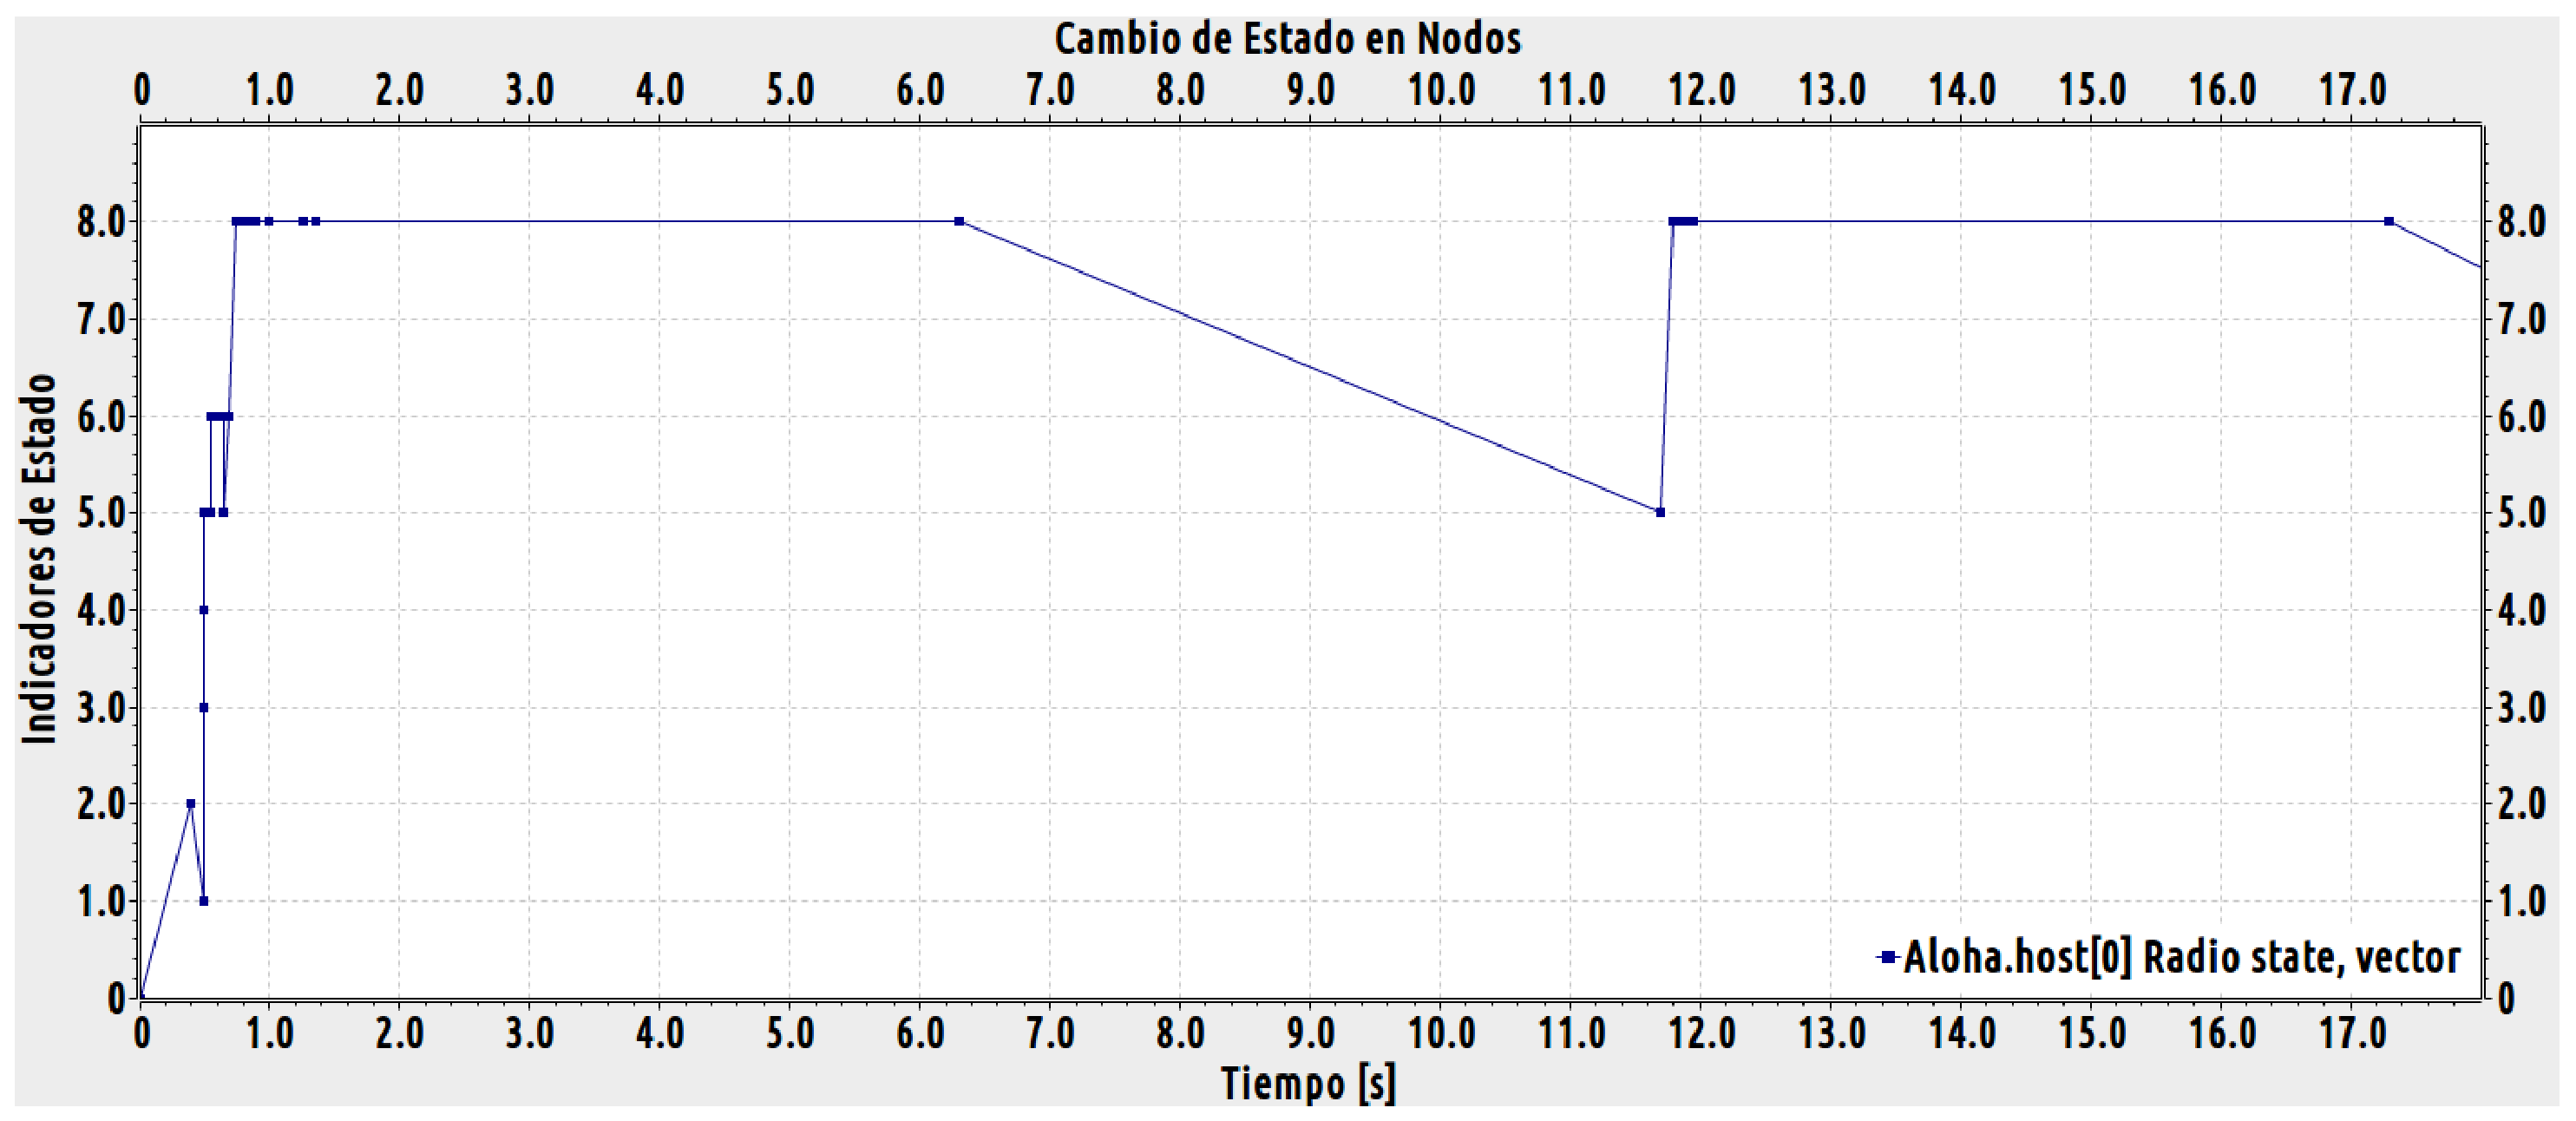
\includegraphics[width=13cm,height=30cm,keepaspectratio]{images/cambioestado1nodo-ideal.eps}
\caption{Gráfico de cambios de estado por tiempo en segundos, con un nodo transmitiendo. \textit{Esta imagen puede verse ampliada en el Anexo~\ref{anexa:1}}}
\label{prueba:1}
\end{figure}
En la Fig~\ref{prueba:2} se encuentra un gráfico de cambios de estado según el tiempo transcurrido, pero esta vez con 10 nodos, con el fin de determinar cuanto demoran los nodos en realizar el proceso de emparejamiento con más nodos por canal.\\
%% pruebas con 10 nodos
\begin{figure}[!ht]
\centering
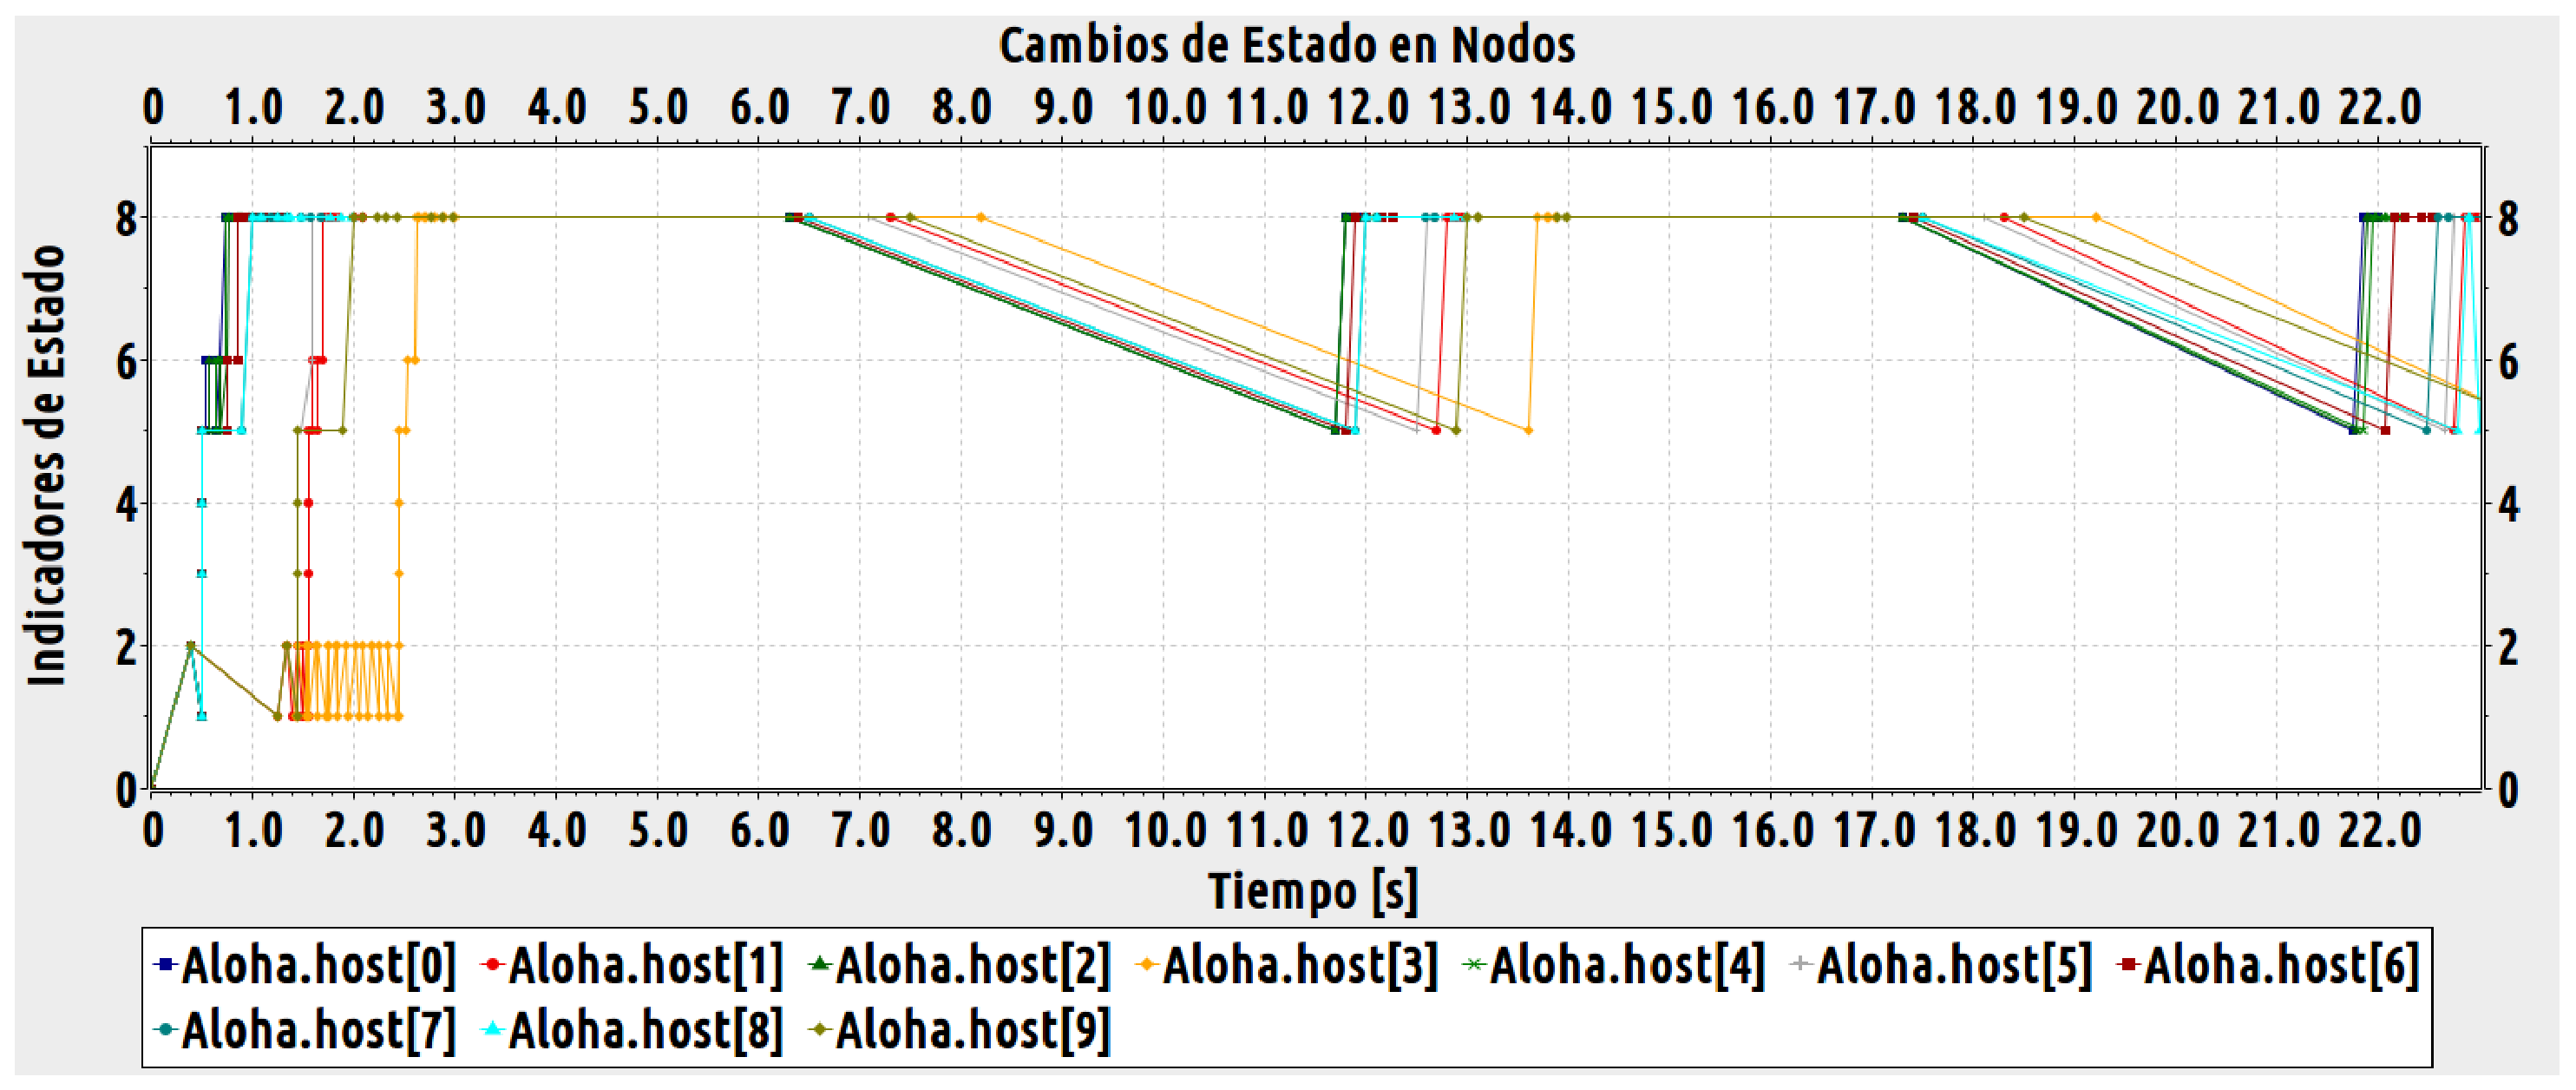
\includegraphics[width=13cm,height=30cm,keepaspectratio]{images/cambioestado10nodos.eps}
\caption{Gráfico de cambios de estado por tiempo en segundos, con diez nodos transmitiendo. \textit{Esta imagen puede verse ampliada en el Anexo~\ref{anexa:2}}}
\label{prueba:2}
\end{figure}
En la Fig~\ref{prueba:3} se presenta un gráfico de cambios de estado donde esta vez se encuentran 100 nodos distribuidos de forma homogénea en los distintos canales disponibles.\newpage \noindent
En estos gráfico, se aprecia de que a medida de que aumenta la cantidad de nodos, el proceso de emparejamiento se ve ralentizado, dado que las colisiones dentro del canal comienzan a generar retransmisiones, las que poco a poco permiten el emparejamiento del total de nodos de la red, y dando inicio al ciclo de transmisión de datos (de medición, u otro tipo) desde los nodos al \textit{gateway}, para luego volver al estado de reposo hasta la próxima ventana de envío.\\
\begin{figure}[!ht]
\centering
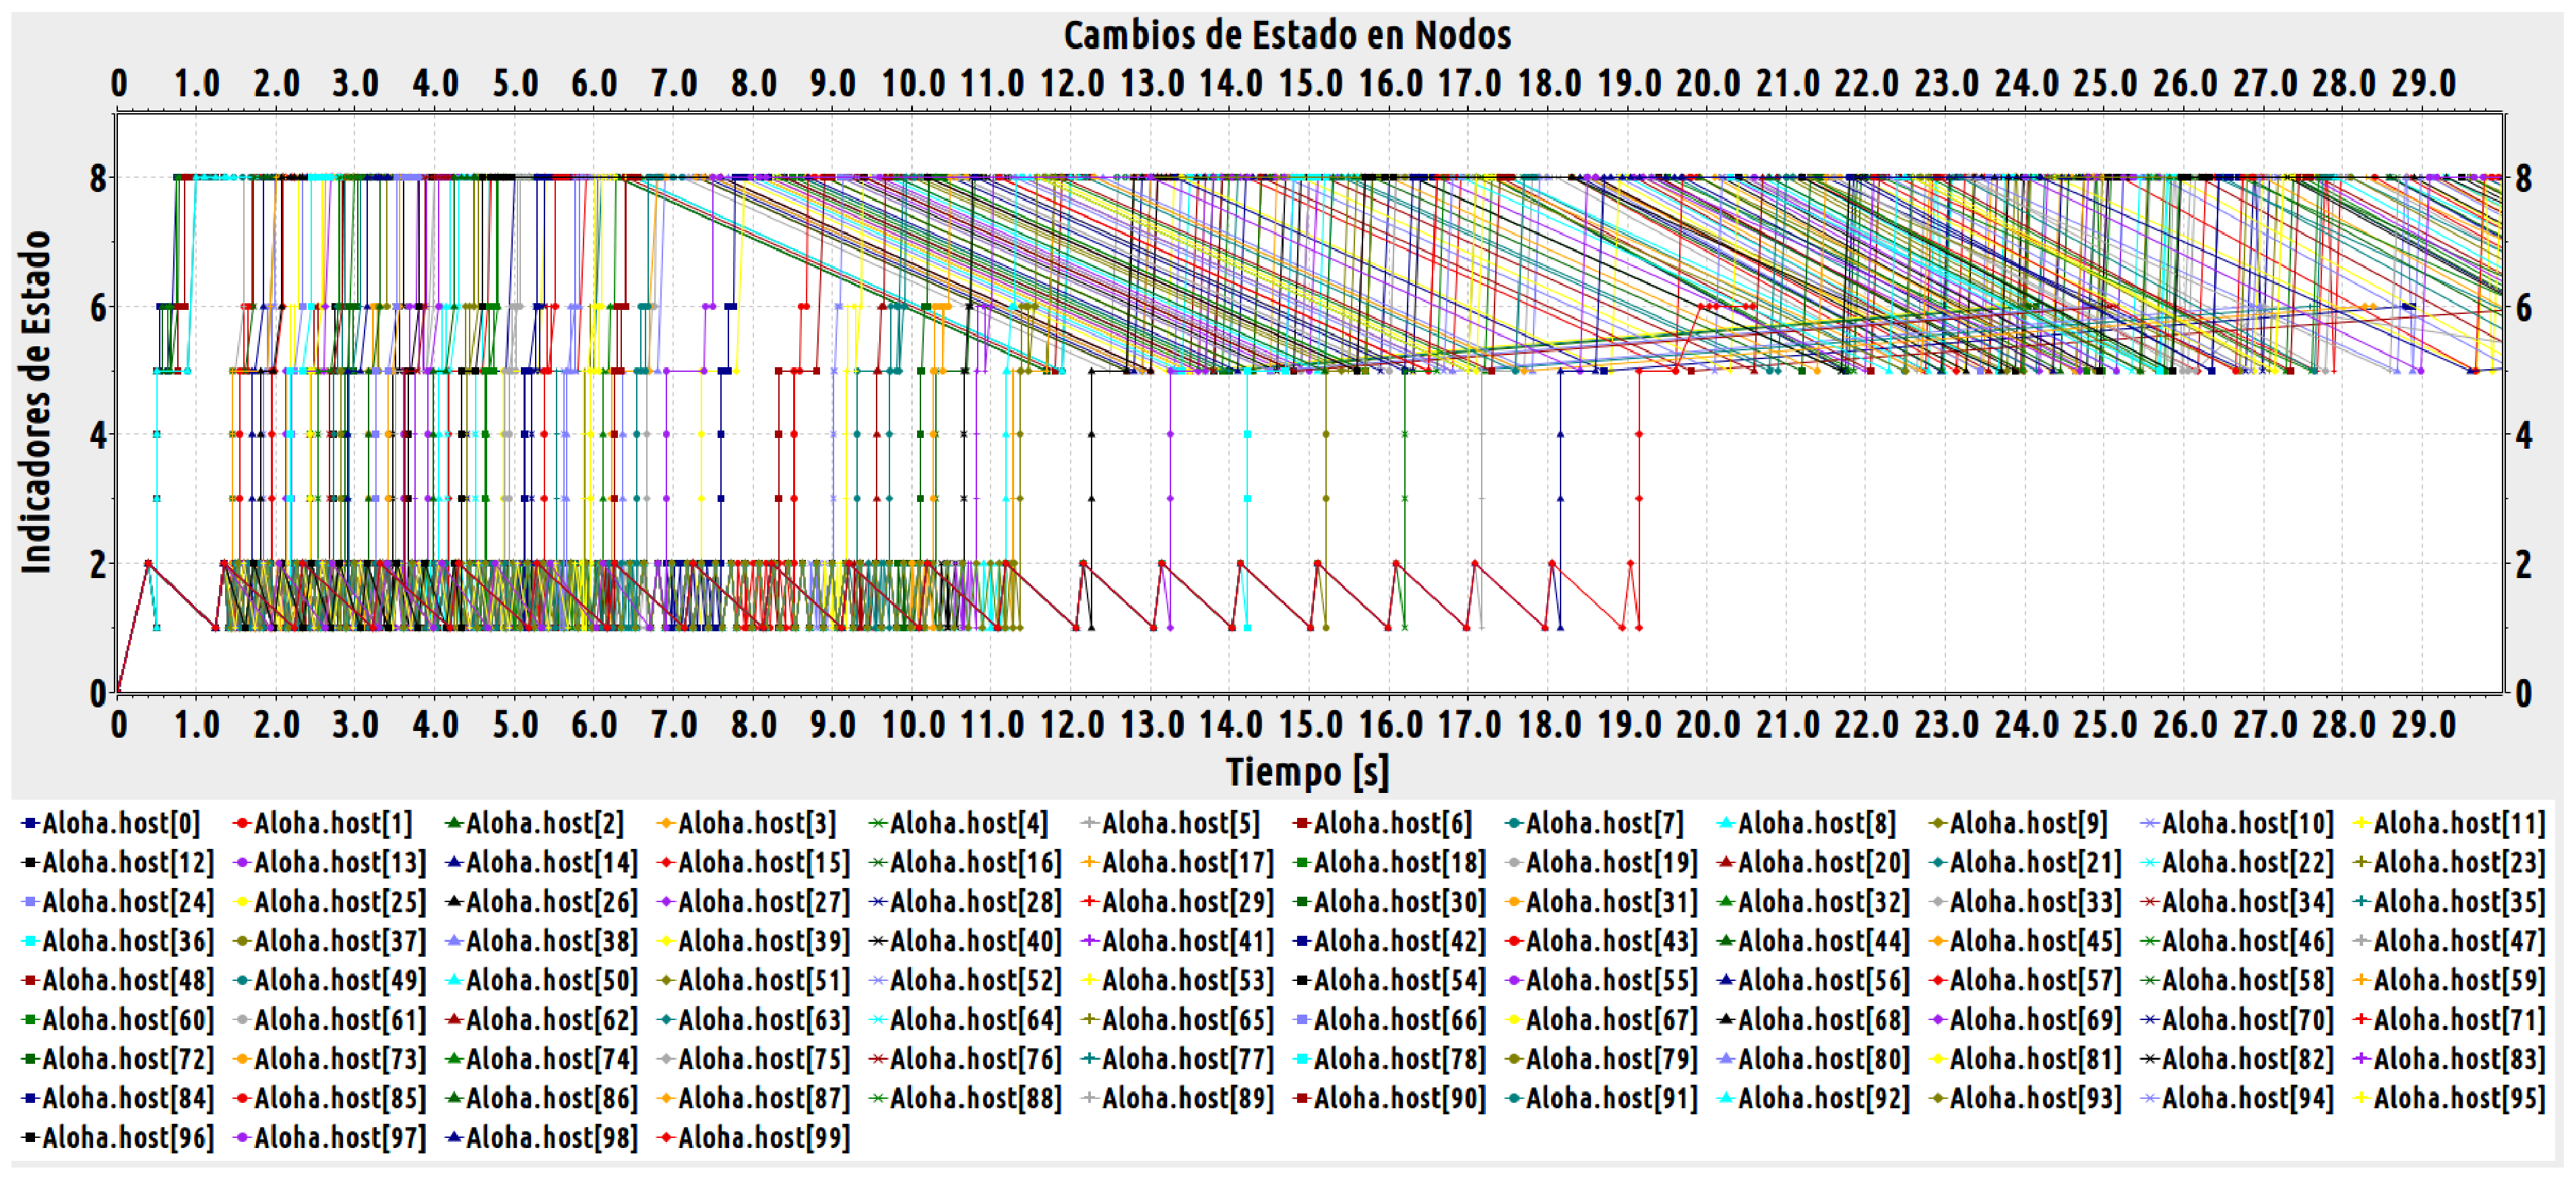
\includegraphics[width=13cm,height=30cm,keepaspectratio]{images/cambioestado100nodos.eps}
\caption{Gráfico de cambios de estado por tiempo en segundos, con cien nodos transmitiendo. \textit{Esta imagen puede verse ampliada en el Anexo~\ref{anexa:3}}}
\label{prueba:3}
\end{figure}
\subsection{Pruebas de transmisión en ambiente virtual}
En estas pruebas, se realizaron transmisiones de datos entre diez y cien nodos durante \SI{60}{\second} de simulación, con el fin de detectar la cantidad de colisiones , por el aumento de la saturación de los canales utilizados. El tiempo de duración de las pruebas de simulación se debe a que en \SI{60}{\second}, es posible visualizar la correcta transición de todos los estados de comunicación presentes en el modelo de simulación, hasta un número de 100 nodos. El valor de la duración de la simulación, fue alcanzado mediante un proceso de optimización de los resultados, donde mediante la realización reiterada de pruebas con resultados no representativos, se alcanzó el tiempo de \SI{60}{\second}. Cabe destacar, que si bien en la simulación transcurre durante \SI{60}{\second}, los gráficos de cambios de estado, sólo muestran dos iteraciones completas del ciclo completo, para evitar mostrar redundancia en los resultados expuestos en los gráficos. No obstante, para el resto de los gráficos, si son utilizados los valores obtenidos durante los \SI{60}{\second} de simulación.\\
Por otra parte, se define el inicio de transmisión de todos los nodos presentes en una simulación, en el mismo segundo. Sin embargo, la herramienta de simulación al mostrar el intercambio de mensajes de forma gráfica, genera una representación gráfica secuencial (sigue el índice asignado a cada nodo y \gls{sf}), es decir, muestra como el intercambio de mensajes se realizará primero en el nodo de índice 0, que en el nodo 1 (a modo de ejemplo), no obstante, esto no se condice con los tiempos de envío de mensajes en la simulación, dado que ambos intentan comunicarse en el mismo segundo, lo que produce que colisionen mensajes y sean reprogramados para la siguiente ventana de envío. En este punto el simulador genera una distribución nuevamente secuencial, sobre cuál nodo calendariza primero su retransmisión, lo que genera un orden secuencial en el envío de mensajes, pero a nivel de programación. Este factor, afecta a los resultados de la simulación de manera negativa, al alejarlos de la realidad, pero se corrigieron al agregar tiempos aleatorios a la calendarización de las próximas programaciones de envío. Lo que se estudió en base a la diferencia de tiempos de envío entre los nodos una vez secuenciados, con el fin de equiparar el ambiente real con el virtual.\\
A través de estas mediciones, se espera visualizar el creciente nivel de retardo en el inicio de las distintas fases de los nodos por efecto de las colisiones, y las retransmisiones inherentes de comunicaciones basadas en el protocolo ALOHA. Cabe decir de que sólo existen colisiones dentro de cada \gls{sf} o canal, ya que entre los distintos \gls{sf} según las especificaciones técnicas  y según las pruebas empíricas realizadas a las capacidades del canal , se indica de que al usar la técnica de modulación de espectro expandido, basta con conocer la frecuencia base del mensaje para poder recibirlo y demodularlo sin problemas, dado que cualquier interferencia en el resto del espectro de la señal, será eliminado al momento de filtrar la señal con un filtro pasa banda, pasa bajo, entre otros, dependiendo del necesario para cada canal~\cite{Sornin}~\cite{Xavier}.\\
En la Fig~\ref{nodos:10}, se observa la cantidad de colisiones por cada \gls{sf}, donde la utilización de cada canal fue aproximadamente de 2 nodos por canal, lo que eventualmente es una saturación muy baja, lo que se traduce en un retardo pequeño en tiempo de el correcto inicio y finalización de los estados correspondientes a cada fase de la comunicación en los dispositivos LoRa.

\begin{figure}[!ht]
\centering
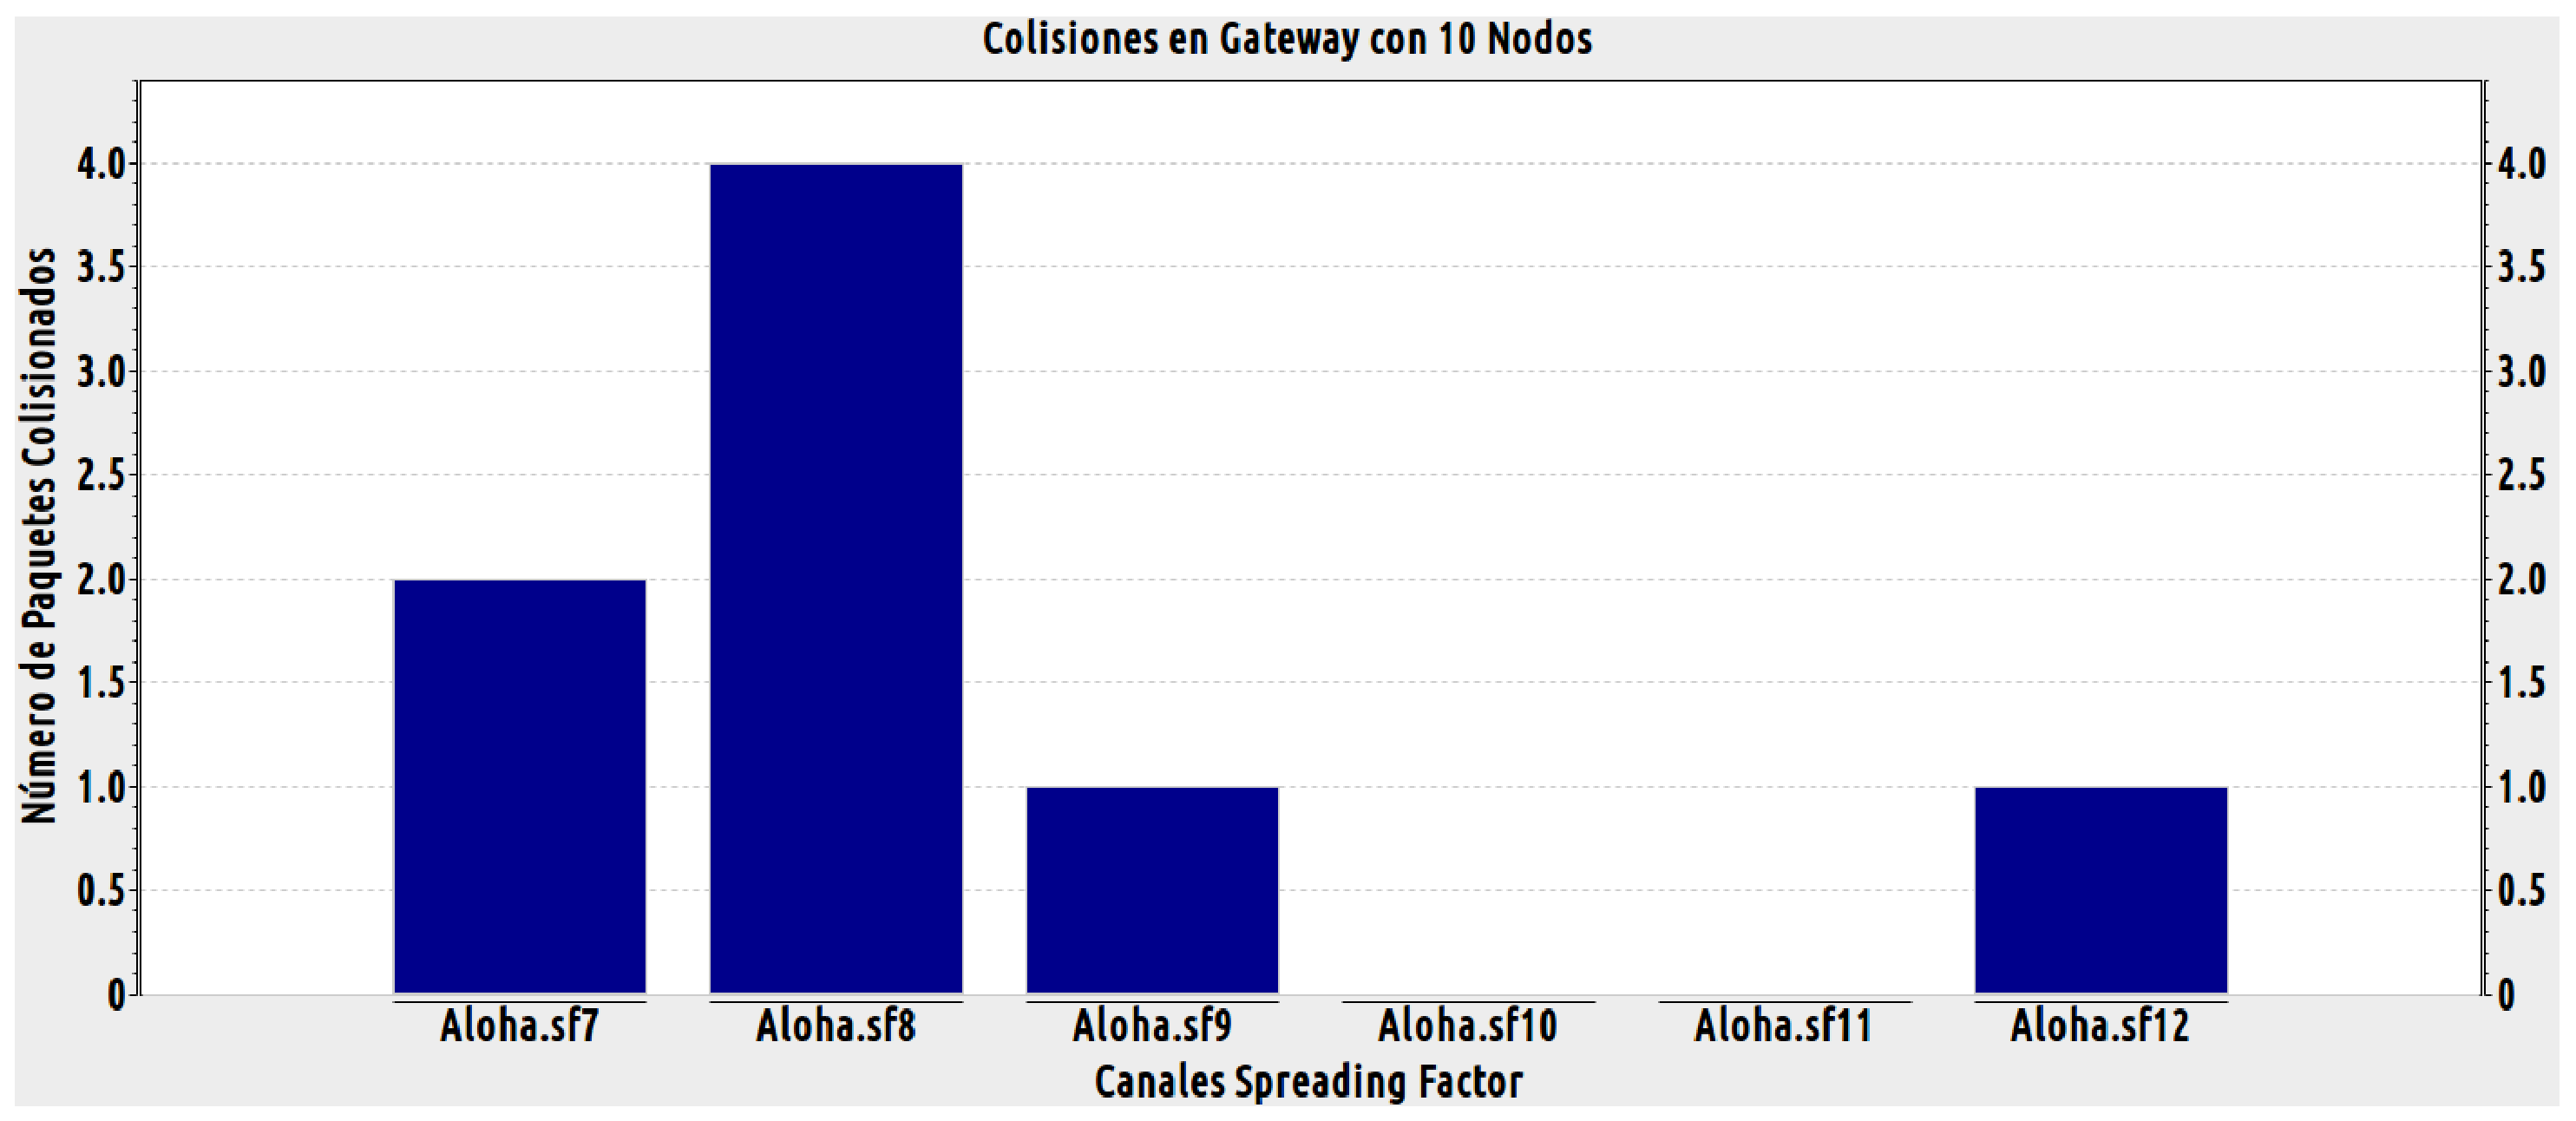
\includegraphics[width=13cm,height=30cm,keepaspectratio]{images/colisiones10nodos.eps}
\caption{Gráfico de colisiones ocurridos entre los distintos \glsentryname{sf}, para 10 nodos transmitiendo. \textit{Esta imagen puede verse ampliada en el Anexo~\ref{anexb:1}}}
\label{nodos:10}
\end{figure}

En la Fig~\ref{nodos:100}, se contempla de que se sigue la misma distribución de colisiones, con la diferencia de que al aumentar los nodos, la saturación del canal  aumenta más de diez veces a la prueba anterior, donde si bien la distribución por canal del número de colisiones se mantiene, la cantidad misma de colisiones no sigue un patrón, lo que puede deberse a un exceso de retransmisiones en el canal produciendo saturación en algún \gls{sf} específico, generando este crecimiento abrupto del número de colisiones. En relación al número de colisiones, estas aumentan también más de diez veces, excepto en el \gls{sf} 8, donde ocurre una anomalía en el comportamiento del modelo de simulación. El cual es explicado por el orden pseudo-aleatorio que posee el \textit{framework} a la hora de indicar que nodo es el siguiente en enviar datos, esto conlleva a que sólo este \gls{sf}, posea este comportamiento fuera de lo normal (como el resto de los \gls{sf}). Adicionalmente, los \gls{sf} 10 y 11, también presentan un crecimiento fuera del patrón (considerando que no habían colisiones con 10 o menos nodos), pero esto tiene relación con el número de nodos por canal, donde la distribución de nodos expuesta en Tab~\ref{tab:prueba} indica de que los canales con sólo un nodo son justamente el \gls{sf} 10 y 11. Esta distribución de nodos por \gls{sf}, se define para probar tanto canales con distribución uniforme, como también la interacción en simultaneo con canales con menor utilización de canal, con el fin de evaluar diferencias de utilización de canal y nivel de colisiones, que es lo que se presenta en este apartado.\\
La diferencia de valores entre \gls{sf} también es explicada por el hecho de que la simulación fue tomada en sólo \SI{60}{s} de simulación, a modo de optimizar los resultados de la medición, dado que en este tiempo, fue posible medir para todos los casos propuestos, el transcurso de todas las fases de comunicación en todos los nodos. Por esta razón, lo que los gráficos muestran, es el estado de la simulación en ese momento dado. Sin embargo, en el caso de haber permitido seguir la simulación una cantidad de segundos más, se apreciaría un emparejamiento del número de colisiones obtenidas en todos los \gls{sf}. Si bien, se realiza esta observación, dado que el \gls{per} agregado al modelo de simulación, recalcula su valor para cada \gls{sf}, cada vez que se recibe un mensaje en cada \gls{sf}. Esto genera, que no se pueda obtener el valor óptimo para esta medición, dado que siempre está recalculando por lo que se entra en un búcle. Por esta razón se estableció un tiempo para tomar la medición de este error, donde en base a prueba y error, se estableció de que a los \SI{60}{s} es posible obtener los mejores resultados para esta prueba (valores más parejos entre los \gls{sf}). Este índice depende mucho de en que fase se encuentren en ese segundo y que evento está queriendo representar. Para este caso en particular, no es importante el hecho de esta anormalidad, dado que se logra explicar el porqué del evento, junto con poder analizar el crecimiento del número de colisiones a mayor número de nodos.
\begin{figure}[!ht]
\centering
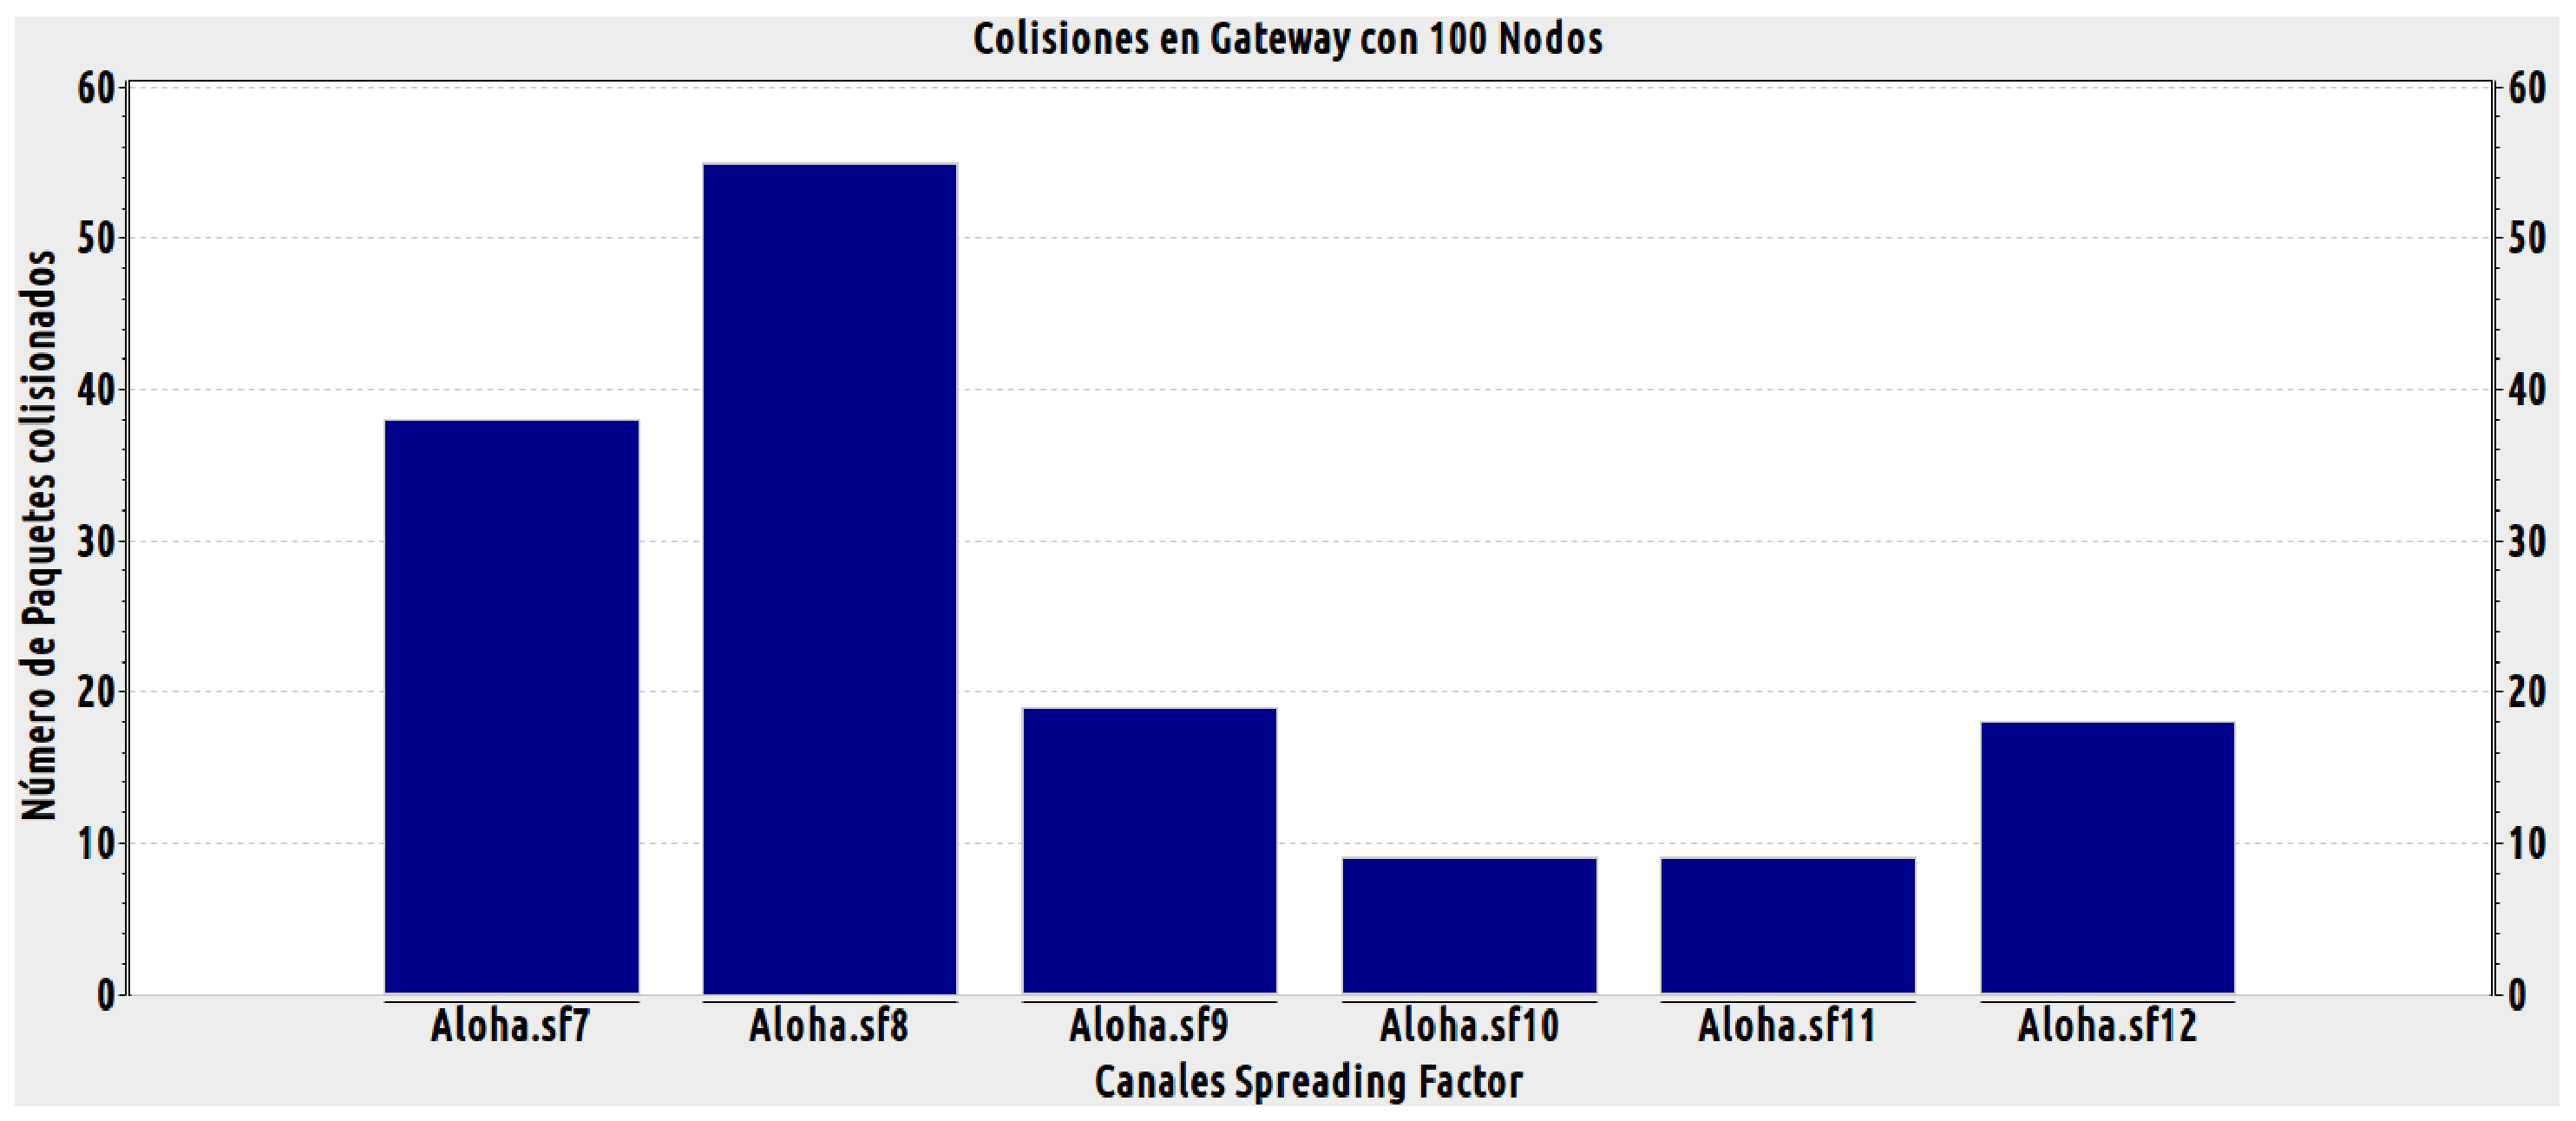
\includegraphics[width=13cm,height=30cm,keepaspectratio]{images/colisiones100nodos.eps}
\caption{Gráfico de colisiones ocurridos entre los distintos \glsentryname{sf}, para 100 nodos transmitiendo. \textit{Esta imagen puede verse ampliada en el Anexo~\ref{anexb:2}}}
\label{nodos:100}
\end{figure}
\subsection{Pruebas de transmisión en ambiente real}
Para realizar las pruebas de transmisión en ambientes reales con los dispositivos LoRa, se utilizó como \textit{gateway} un concentrador LoRa c880A con una antena omnidireccional que trabaja en la banda de frecuencia \SI{868}{\mega\hertz}, que posee \SI{5}{dbi} de sensibilidad, adicionalmente se transmitió con una potencia de \SI{10}{dbm}. Este dispositivo fue conectado a una Raspberry Pi 2. Como nodo se utilizó un inAir9 (LoRa Module \SI{868}{\mega\hertz}), el que tuvo conectada una antena omnidireccional con una sensibilidad de \SI{5}{dbi} y tuvo configurada una potencia de transmisión de \SI{10}{dbm}. El nodo se conectó a un arduino UNO el que funcionó como \textit{backend}. La distancia entre el nodo y el \textit{gateway} fue de \SI{20}{\meter} aproximadamente sin obstaculos entre ellos. En relación a la altura del \textit{gateway}, esta fue de \SI{1.2}{\meter} aproximadamente, la que se debe a la altura de una mesa, ubicada en las áreas verdes de la facultad de ingeniería de la Universidad Diego Portales. Por otro lado la del nodo fue de \SI{0.9}{\meter} aproximadamente, altura debida al bloque de cemento utilizado como base del nodo.\\
Las pruebas de transmisión, se realizaron cinco veces para cada \gls{sf}, con el fin de determinar el porcentaje de pérdida de paquetes en cada espectro de frecuencia y agregarlo al modelo de simulación. \noindent
La cantidad de iteraciones del experimento de transmisión, se debe a un proceso de optimización en los resultados del experimento, es decir, a medida que se realizaron las mediciones, se procedió a ajustar el número de iteraciones sobre la base de los resultados obtenidos. Como puede apreciarse en Tab~\ref{prueba:real}, en esta prueba se enviaron en promedio noventa y siete paquetes de datos, de los cuales sólo se recibió alrededor de treinta y siete en promedio, lo que corresponde a un \SI{38}{\percent} de recepción de los datos enviados en el total de paquetes enviados. Sin embargo, algunos resultados en las mediciones tuvieron una diferencia considerable de resultados (véase [*] en Tab~\ref{prueba:real}), valores que son explicados si se toma en cuenta que los valores expuestos en la tabla de resultados son promedios de todas las pruebas realizadas por cada canal de comunicaciones, donde cabe destacar, que las intensidades de las interferencias a las que estaban sometidos los dispositivos al momento de las mediciones eran variables, lo que explica el por qué el valor en el \gls{sf}9 posee una desviación alta en comparación con los valores de los otros canales. Los valores que provocan esta desviación en el \gls{sf}9, no fueron quitados con el fin de mostrar de que en algunos casos se lograron valores de recepción altos en las mediciones, con respecto a la pérdida de paquetes (valores bajo el \SI{10}{\percent} en \gls{per}), como también valores bajos en relación a la recepción de paquetes (valores de \gls{per} sobre el \SI{70}{\percent}). Estos resultados en la mayoría de los casos, mostraron una tendencia a obtener valores de \gls{per} altos, excepto en el canal \gls{sf}9, donde hubo una mayor incidencia de recepción exitosa de mensajes que en el resto de canales.\\
La configuración de parámetros usada para esta prueba, junto con la arquitectura de red usada corresponden a los valores y distribuciones definidos en la sección~\ref{sec:param}. A continuación se presentan los resultados:
\begin{table}[!ht]
\centering
\begin{tabular}{|c|c|c|c|}
\hline
\gls{sf} & Paquetes enviados & Paquetes recibidos & Paquetes perdidos \SI{}{\percent} \\ 
\hline
SF12 & 84 & 30 & \SI{65,1}{\percent}\\
\hline
SF11 & 99 & 15 & \SI{84,8}{\percent}\\
\hline
SF10 & 158 & 19 & \SI{87.9}{\percent}\\
\hline
SF9 & 360 & 78 & \SI{78.3}{\percent}[*]\\
\hline
SF8 & 469 & 38 & \SI{91.9}{\percent}\\
\hline
SF7 & 983 & 47 & \SI{95.2}{\percent}\\
\hline
\end{tabular}
\caption{Tabla con resultados de pruebas de conectividad por \glsentryname{sf}}
\label{prueba:real}
\end{table}
\newpage \noindent
Bajo este contexto, estos resultados sirvieron para el modelado de los dispositivos LoRa, dado que en un principio se definió que se dejaría un valor fijo de pérdida de paquetes para representar el estándar expuesto en las especificaciones de los desarrolladores de LoRa, sin embargo, estos resultados revelaron de que la variabilidad de resultados respecto a la recepción de datos, depende de tres factores principales: la potencia de transmisión, la sensibilidad de recepción y el uso del espectro expandido. En relación a estos antecedentes, se estableció de que se modelaría de forma dinámica la pérdida de paquetes, con el fin de adaptar el modelo de simulación a cualquier tipo de ambiente a simular, sin que este pierda similitud con el comportamiento real en los dispositivos.
\subsection{Índice de pérdida de paquetes}
En relación a las pruebas de transmisión realizadas con los dispositivos físicos, se alejan mucho de los resultados esperados, e incluso de los datos que otorga la especificación de LoRa. Esto es causado por la interferencia generada por la fuente de poder administrada a los dispositivos y una incorrecta forma de aislamiento de los conectores y partes conductoras de la placa. Adicionalmente, se considera de que que sea producto de la baja potencia de transmisión del \textit{gateway} (\SI{5}{dbm}), e incluso de la alta sensibilidad de la antena de transmisión (\SI{5}{dbi}) dado que esto la hace más permeable a interferencias ambientales propias de una universidad. Adicionalmente, se considera la baja altura a la que se colocó el \textit{gateway} (\SI{1.2}{\meter}), como un factor negativo en las mediciones, dado que los dispositivos estuvieron a baja altura, estos pudieron ser afectados por radiación de electrodomésticos. Por otra parte, todas las pruebas realizadas por investigadores, tanto las pruebas realizadas a la capacidad del canal, como a la capacidad de transmisión, los resultados arrojan que sus pruebas son muy satisfactorias dado que sus resultados, se apegan a las especificaciones técnicas entregadas por Semtech en condiciones dentro de las normas expuestas allí.\newpage \noindent 
Dentro de las características de estas pruebas, se encuentra que los \textit{gateway} están ubicados a una altura de sobre los \SI{20}{\meter} en torres fijas, y equipados con antenas bi-cónicas con una sensibilidad de \SI{2}{dbi}, y transmitiendo a una potencia de (\SI{14}{dbm}), lo que permite una transmisión a mucha más distancia que el mismo \textit{gateway} a una menor altura, donde la calidad de transmisión puede verse mermada por las interferencias a ese nivel de altura, agregando a este análisis, de que las antenas utilizadas en los experimentos expuestos en los artículos citados, están diseñadas para la comunicación direccional en sus dos polos, lo que aumenta el nivel de emisión y recepción en estas direcciones, a diferencia de la omni direccional que se utilizó para estas mediciones, que posee un mayor nivel de pérdida en ciertos polos~\cite{Xavier}~\cite{Juha}~\cite{NORMAN}.\\
De acuerdo a este contexto, se decidió adoptar el porcentaje de pérdida de paquetes que entregan las distintas mediciones realizadas por otros investigadores (tasa de pérdida de paquetes = \SI{1}{\percent}), se asemejan más a la norma y a las especificaciones~\cite{Xavier}~\cite{Juha}.

\subsection{Resultados obtenidos agregando pérdida de paquetes}
Dentro de las pruebas de transmisión en el ambiente virtual, también se registró la cantidad de paquetes con errores (que no llegaron a destino), los que en un ambiente real pueden tener el carácter de interferencia. Para el modelo de simulación el porcentaje de pérdida en la recepción de datos, se mide en cada transmisión en base al \gls{per} ingresado, junto a la cantidad de paquetes recibidos por cada \gls{sf}, por lo que dependiendo de que \gls{sf} posea más envíos efectivos de mensajes (en el caso de que uno haya entrado antes al estado de transmisión que otro nodo).\\
Como es posible notar en la Fig~\ref{prueba:4}, la cantidad de envíos de datos con errores es igual en los \gls{sf}7, 8 y 12 (con un \gls{per} del \SI{1}{\percent}), excepto en los \gls{sf}9 \gls{sf}10 y \gls{sf}11 donde se presenta un valor menor. Ésto es debido a que los \gls{sf} afectados, transmitieron entre 10-50 paquetes menos que el resto de los \gls{sf}. Cabe mencionar de que, en el caso de que la simulación hubiera continuado, es posible de que el índice \gls{per} se hubiera vuelto homogéneo en todos los \gls{sf}.\\
Estos resultados al ser satisfactorios demuestran de que, con diez nodos, la función que calcula esta pérdida es efectiva dependiendo del número de paquetes recibidos, por lo que se concluye que es efectiva en un nivel bajo de saturación de canal (bajo 50 nodos por canal).
%%pruebas con 5 nodos
\begin{figure}[!ht]
\centering
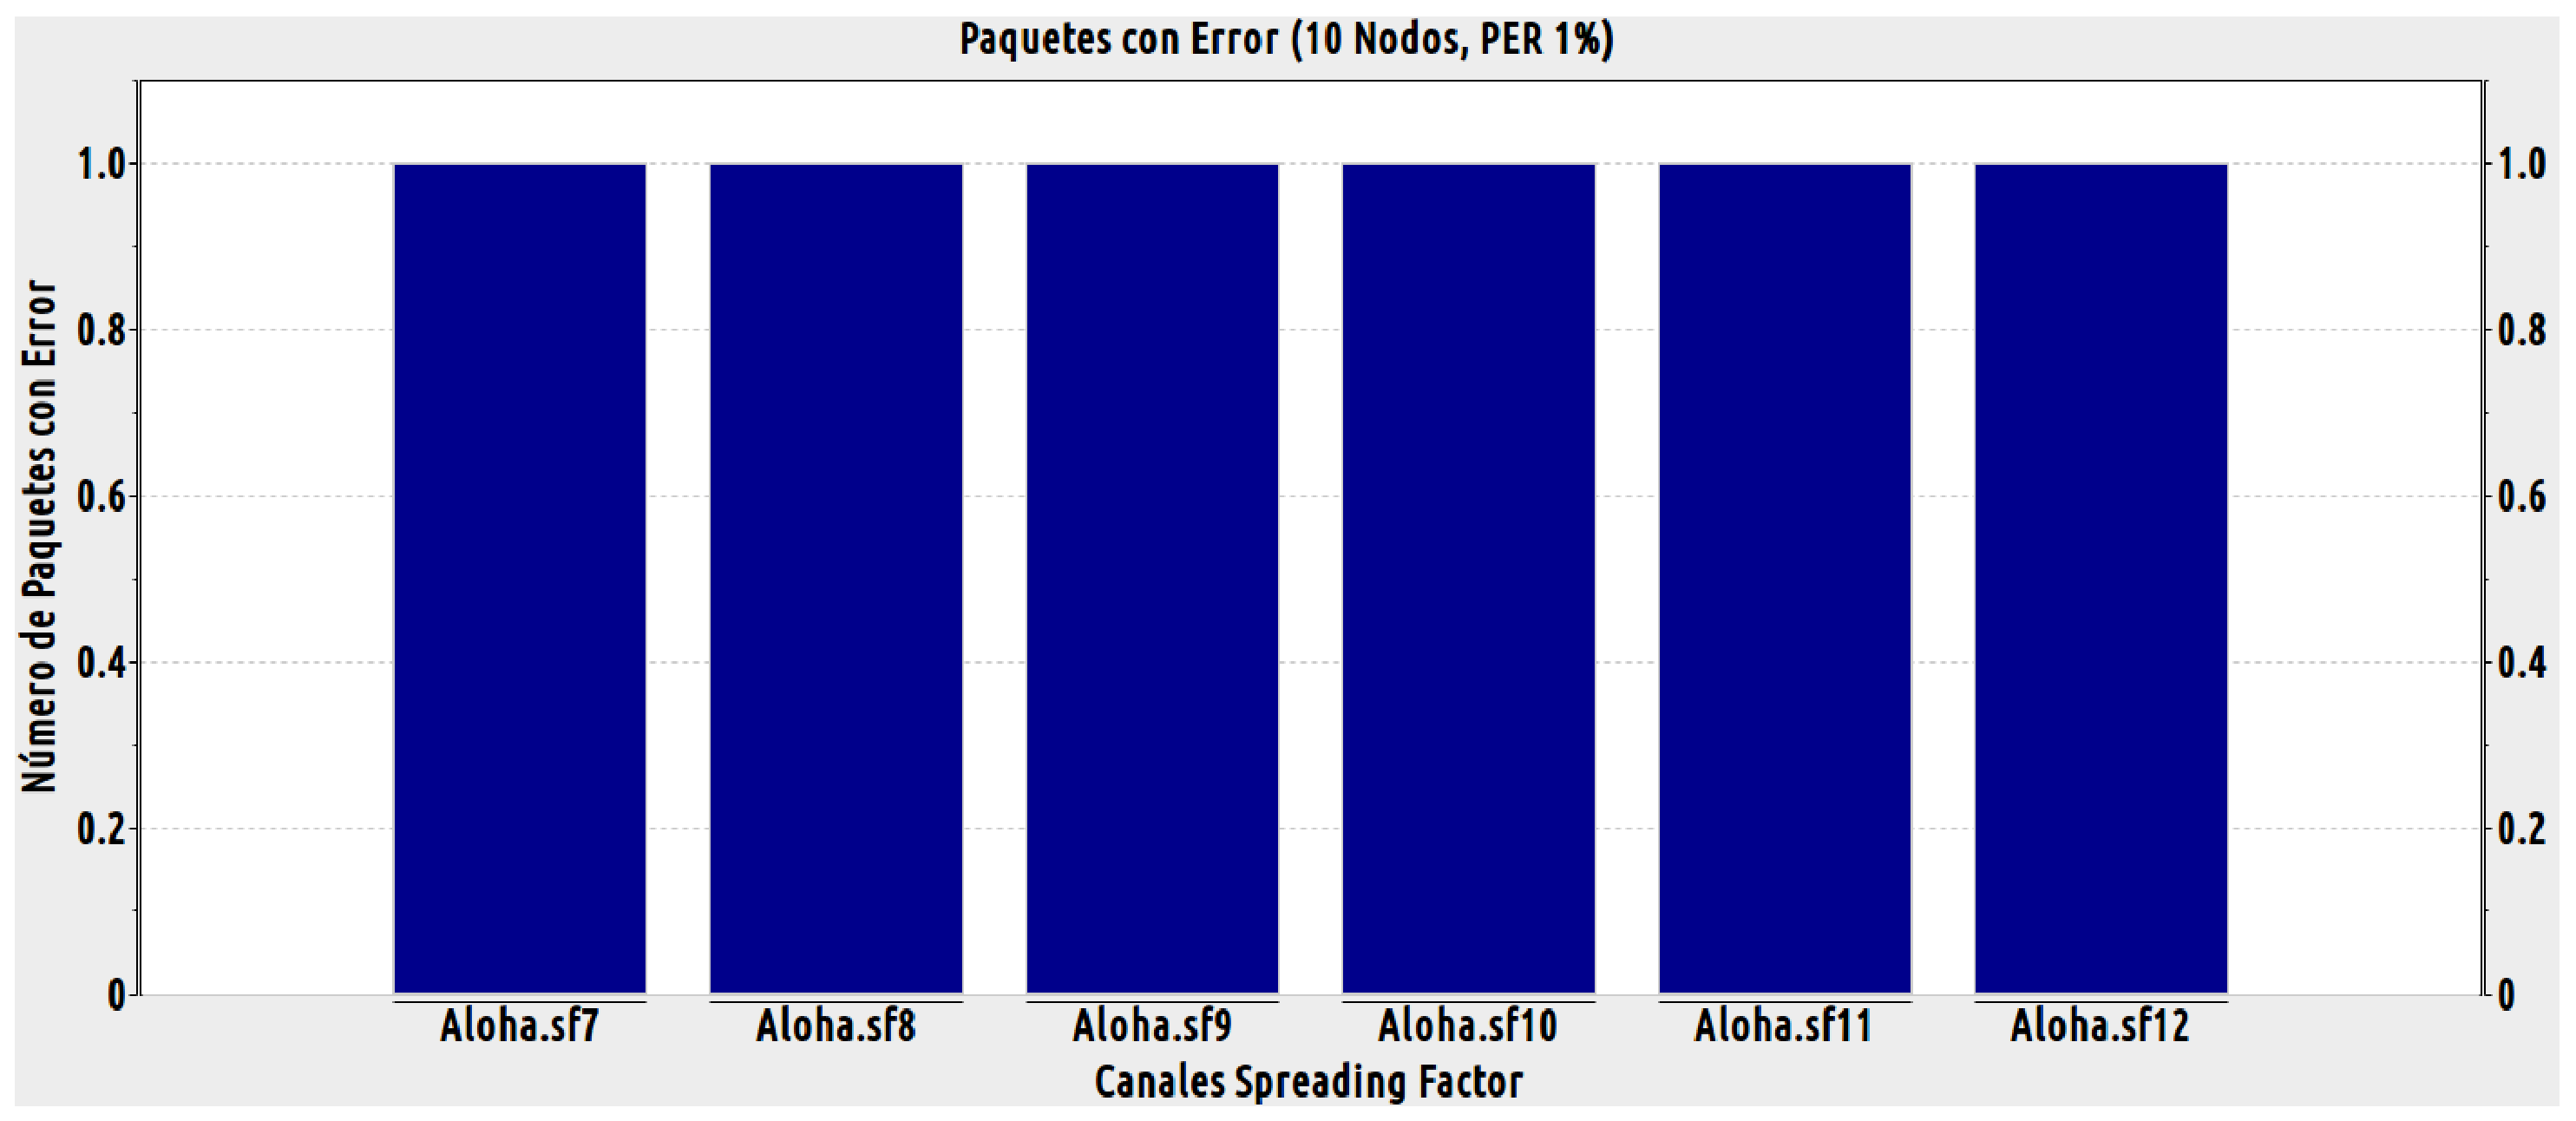
\includegraphics[width=13cm,height=30cm,keepaspectratio]{images/errores10nodos.eps}
\caption{Gráfico de cantidad de paquetes con errores en cada \glsentryname{sf} en la simulación, para 10 nodos. \textit{Esta imagen puede verse ampliada en el Anexo~\ref{anexb:3}}}
\label{prueba:4}
\end{figure}\newpage \noindent
Sin embargo, en la Fig~\ref{prueba:5}, se evidencia un aumento considerable en la cantidad de paquetes con errores, donde la distribución ya no se hace tan homogénea como para el caso de diez nodos. Esto ocurre dado que por las colisiones y el orden arbitrario del simulador \OMNET, donde algunos nodos pertenecientes a determinados \gls{sf} (en este caso particular, el \gls{sf}\num{8}), poseen oportunidades más recurrentes de transmisión que otros, por lo que genera de que algunos \gls{sf} posean una cantidad menor del \SI{1}{\percent}, lo que es esperable, como también que en otros casos, supera el \SI{1}{\percent}. Este evento es debido a que al momento de tomar el estado de la simulación, esta función no terminaba de acomodar el índice de recepción de datos con error al \SI{1}{\percent}, ya que la función que calcula éste índice, a medida que llegan paquetes de forma íntegra al \gls{sf}, este aumenta un contador de envíos recibidos, por lo que al calcular el porcentaje de recepciones con error, este comienza a disminuir de forma paulatina, hasta que disminuye bajo el valor asignado de \gls{per}. Cuando esto ocurre, la función desecha el siguiente paquete en el \gls{sf}, aumentando con esto en uno el contador de recepciones con error y por consecuencia el índice \gls{per}, donde nuevamente sigue calculando de forma cíclica hasta que el porcentaje disminuye hasta el valor asignado al \gls{per}.\newpage \noindent Este evento al no presentarse en todos los \gls{sf} por igual, no se atribuye una falla de diseño, o una falla del simulador, por lo que se presenta como anomalía que depende del tiempo cuando es detenida la simulación al momento de tomar datos estadísticos que representen el comportamiento de los dispositivos.\\
Este evento anómalo ocurre de forma análoga para la incongruencia en las colisiones para 100 nodos.

\noindent
\begin{figure}[!ht]
\centering
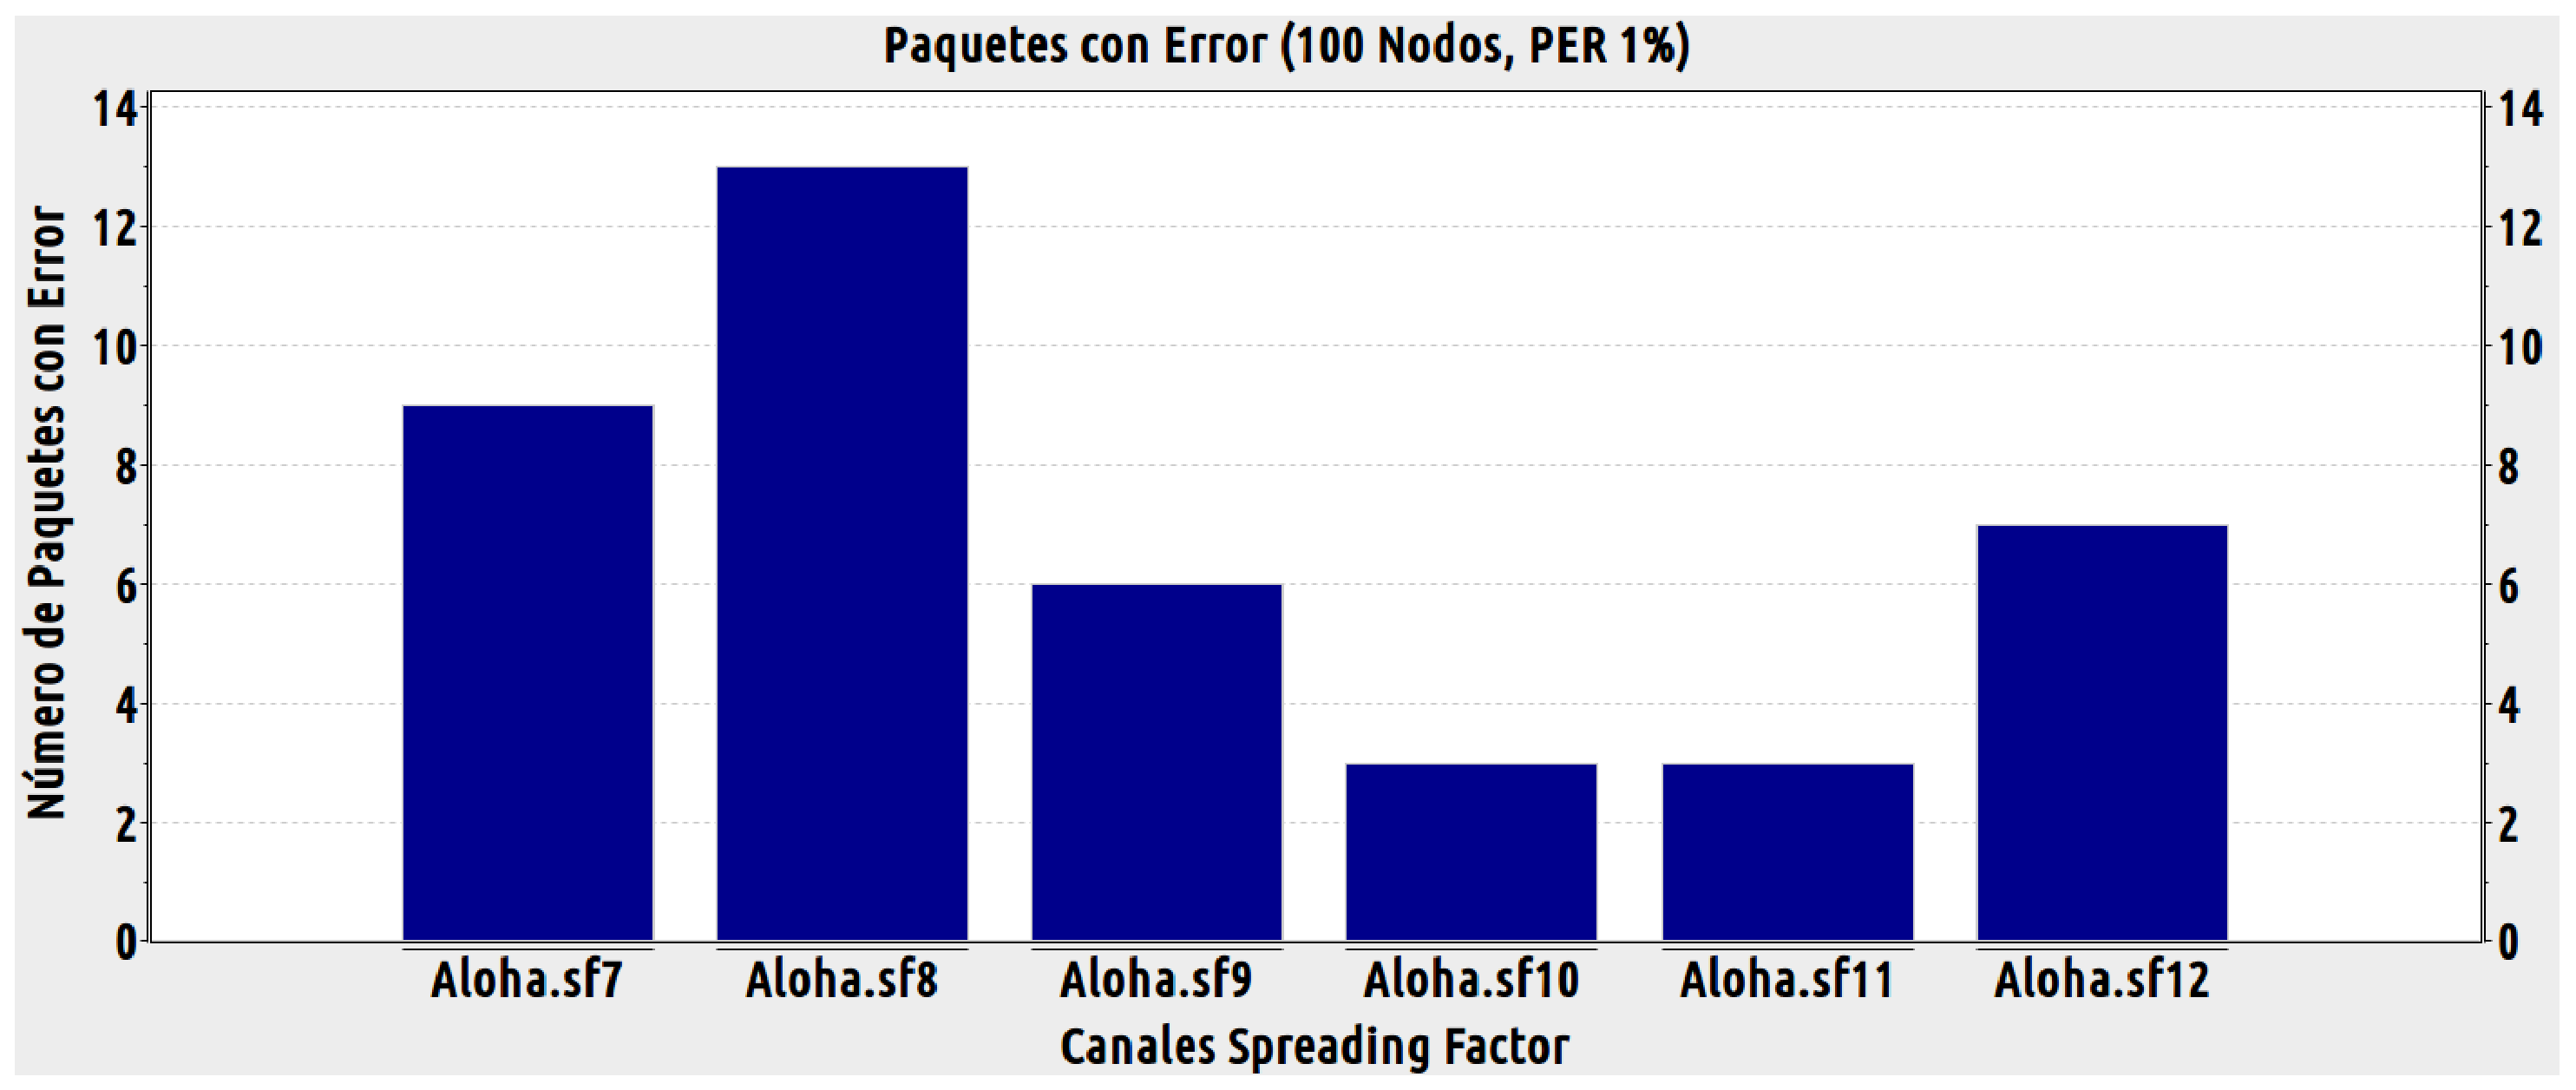
\includegraphics[width=13cm,height=30cm,keepaspectratio]{images/errores100nodos.eps}
\caption{Gráfico de cantidad de paquetes con errores en cada \glsentryname{sf} en la simulación, para 100 nodos. \textit{Esta imagen puede verse ampliada en el Anexo~\ref{anexb:4}}}
\label{prueba:5}
\end{figure}
\end{justify}
\justify
%%%%CONCLUSION%%%%%%
\begin{justify}
\chapter{Conclusiones}
En cuanto a el diseño e implementación del modelo de simulación desarrollados en este proyecto, se puede decir que la implementación del modelo de simulación, logra imitar de forma análoga el comportamiento de los dispositivos LoRa en relación a su funcionamiento lógico y físico, dado que logra simular cada fase de comunicación de los dispositivos LoRa, como la fase de emparejamiento, transmisión/retransmisión y la fase de descanso en nodos. De esta misma forma se imitó el funcionamiento físico de los dispositivos, lo que se pudo realizar implementando funciones que simulan de forma análoga el comportamiento de la tasa adaptativa de envío de datos. En las funciones que simulan el comportamiento del \gls{adr}, se analiza la distancia entre el nodo y el \textit{Gateway} de forma dinámica para asignar el canal (\gls{sf}) adecuado para dicha , cambiando con esto la tasa de envío de datos correspondiente al canal asignado. Adicionalmente se logró implementar una función que simula la pérdida de paquetes, donde en base a un \gls{per} asignado, esta función calcula si es necesario o no descartar un paquete en cada canal para cumplir con el \gls{per} asignado.\\
La implementación de este modelo de simulación muestra el cómo se realiza la comunicación de los dispositivos LoRa en una red de topología estrella, donde es posible probar tanto distribuciones de nodos en los distintos canales o \gls{sf}, como también el rendimiento de los dispositivos al agregarle variables reales como el porcentaje de la pérdida de paquetes, o la asignación dinámica de la tasa de envío, tomando la distancia que posee el nodo hasta el \textit{Gateway}.\\
En la implementación del módulo de transición LoRaWAN/IPv6, se logró la correcta adquisición de la información, tanto de los dispositivos de la red LoRa, como del \textit{Payload} que se busca transmitir hacia un servicio de carácter web como lo es una Base de datos. Dado que este módulo de transición es implementado en base al uso de \glspl{socket}, es posible agregar, dependiendo de las necesidades del desarrollador, una capa de cifrado a los datos usando OpenSSL u TLS para comunicarse con los servidores objetivo, donde en el caso de agregar cifrado, se estaría además añadiendo una capa de seguridad adicional a la existente actualmente (cifrado sobre el mensaje), al usar el método de retransmisión de paquetes hacia el computador remoto, el cual sólo realiza una condición \textit{Pass Through} en el \textit{Firewall} local.\\
\noindent
En relación al desarrollo del modelo de simulación, este se caracteriza por aportar la capacidad de realizar pruebas de conectividad de dispositivos LoRa, con distintas distribuciones y con diferentes configuraciones de parámetros (\gls{per}, tasa de envío de datos, etc.) en un ambiente virtual, obteniendo resultados análogos a los que se obtendrían con una medición en un ambiente real. No obstante, la topología abarcada en este proyecto es la topología estrella, este modelo no admite distribuciones estrella-de-estrellas ni variantes más complejas, por lo que este aporte iría enfocado en redes simples con un \textit{Gateway} único en la red.\\
En cuanto al módulo de transición, este otorga la capacidad de poder interconectar de forma directa una red LoRa con un servicio de red, teniendo la posibilidad de agregar o no, una capa de seguridad extra al canal de transmisión hacia Internet.
\end{justify}
% Iniciamos el resto de secciones adicionales al contenido: referencias y apendices
\backmatter
% Bibliografía
% referencias.bib es el archivo con la base de datos bibliografica
% se recomienda utilizar un manejador de referencias: Jabref (jabref.sourceforge.net)
% El estilo por defecto es IEEE Transactions
\bibliographystyle{IEEEtran}
% Acá puede incluir uno más archivos de referencia
\bibliography{IEEEabrv,tubiblio}
% Simbología y glosario
% Utilice un paquete para generar símbolos y glosarios.
% Por ejemplo: nomencl (http://texdoc.net/pkg/nomencl)
%%%glosario%%%
%definicion de terminos
%%glosario
\newglossaryentry{iotg}{name={Internet of Things}, description={IoT es el término usado en ciencias de la computación, para referirse a la integración de los protocolos IPv4 o IPv6, en dispositivos que no fueron inicialmente diseñados para realizar una conectividad mediante el uso de Internet, esto se realiza con el fin de poder ampliar la diversidad de usos y aplicaciones que pueden llegar a tener dispositivos de esta naturaleza}}

\newglossaryentry{lpwang}{name={LPWAN}, description={Las LPWAN, son todas aquellas redes inalámbricas, diseñadas para permitir comunicaciones de largo alcance a una baja tasa de envío de bits}}

\newglossaryentry{lorawang}{name={LoRaWAN}, description={LoRaWAN, es el protocolo utilizado en las redes LPWAN de la familia de los LoRa, el que tiene la cualidad de optimizar el funcionamiento de ALOHAnet utilizando una programación de mensajes en base al tiempo, y junto con esto, el uso de multi canales de comunicación para evitar colisiones y asegurar una conectividad con el menor grado de pérdidas. Aunque, también este acrónimo es utilizado para hacer referencia a las redes LPWAN de la familia de los LoRa}}

%%acrónimos
\newglossaryentry{iot}{type=\acronymtype,  name={IoT}, description={\textit{Internet of Things}}, first={IoT(\textit{Internet of Things})\glsadd{iotg}}, see=[Glosario:]{iotg}}

\newglossaryentry{lorawan}{type=\acronymtype,  name={LoRaWAN}, description={\textit{Long Range Wide-Area Network}}, first={LoRaWAN(\textit{Long Range Wide-Area Network})\glsadd{lorawang}}, see=[Glosario:]{lorawang}}

\newglossaryentry{lpwan}{type=\acronymtype,  name={LPWAN}, description={\textit{Low Power Wide-Area Network}}, first={LPWAN(\textit{Low Power Wide-Area Network})\glsadd{lpwang}},  see=[Glosario:]{lpwang}}

%%acronimos
\glsaddall
\printglossary[type=\acronymtype]

\printglossary[type=main]
% Anexos
\appendix


%asd
%%pruebas con 5 nodos
\chapter{Anexo A}
%%pruebas con 5 nodos

\begin{figure}[!ht]
\centering
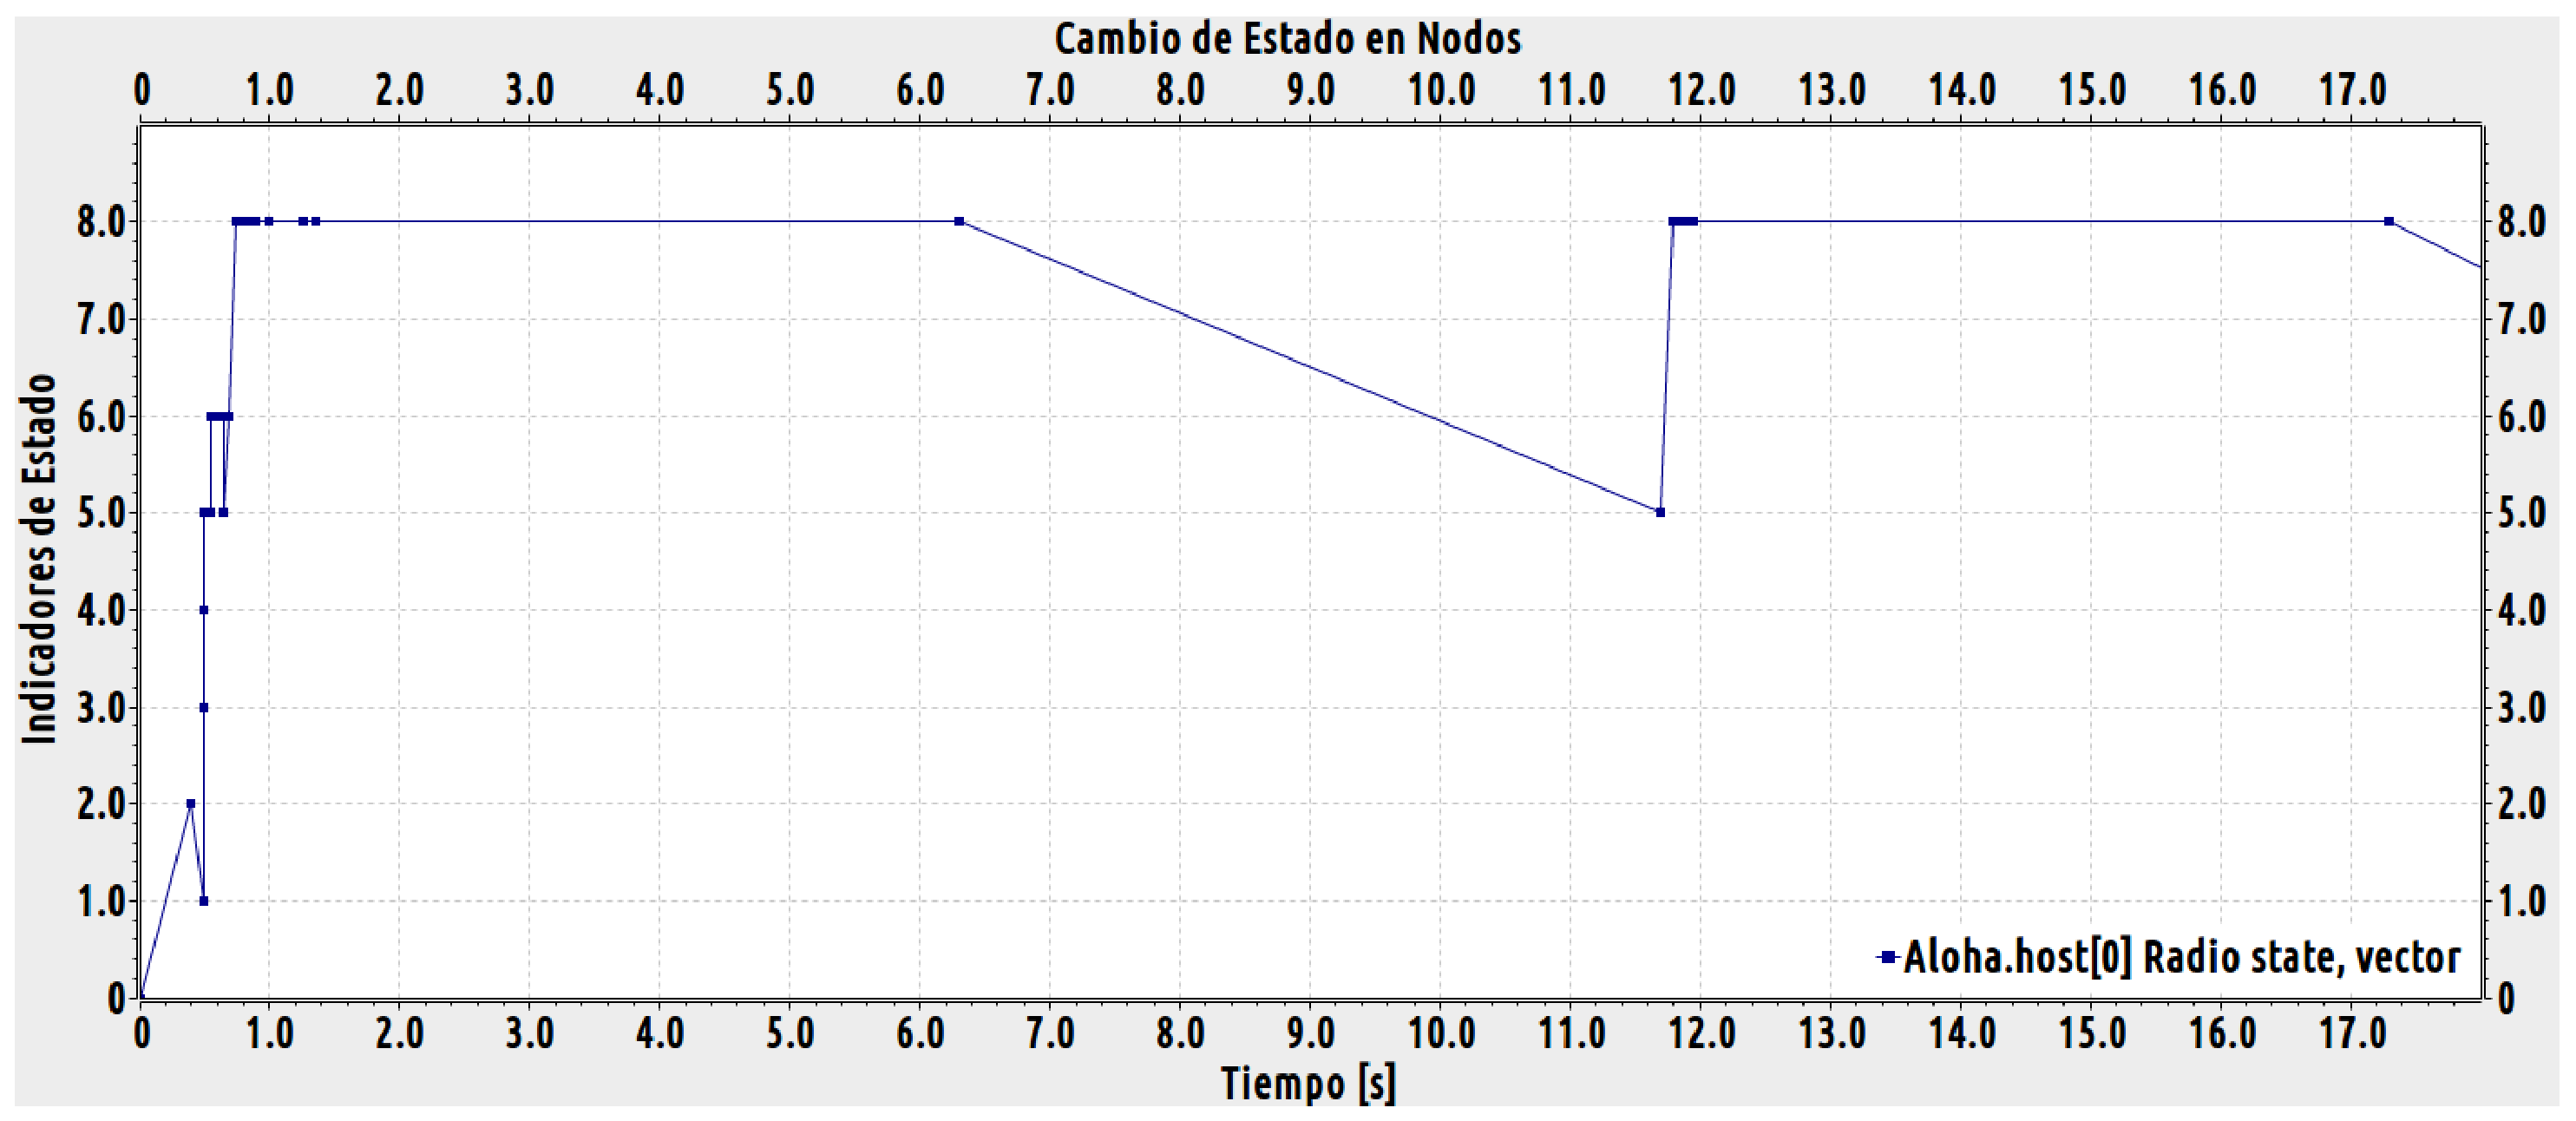
\includegraphics[angle=270, scale=0.4]{images/cambioestado1nodo-ideal.eps}
\caption{Gráfico de cambios de estados por tiempo en segundos, con un nodos transmitiendo}
\label{anexa:1}
\end{figure}

%% pruebas con 50 nodos
\begin{figure}[!ht]
\centering
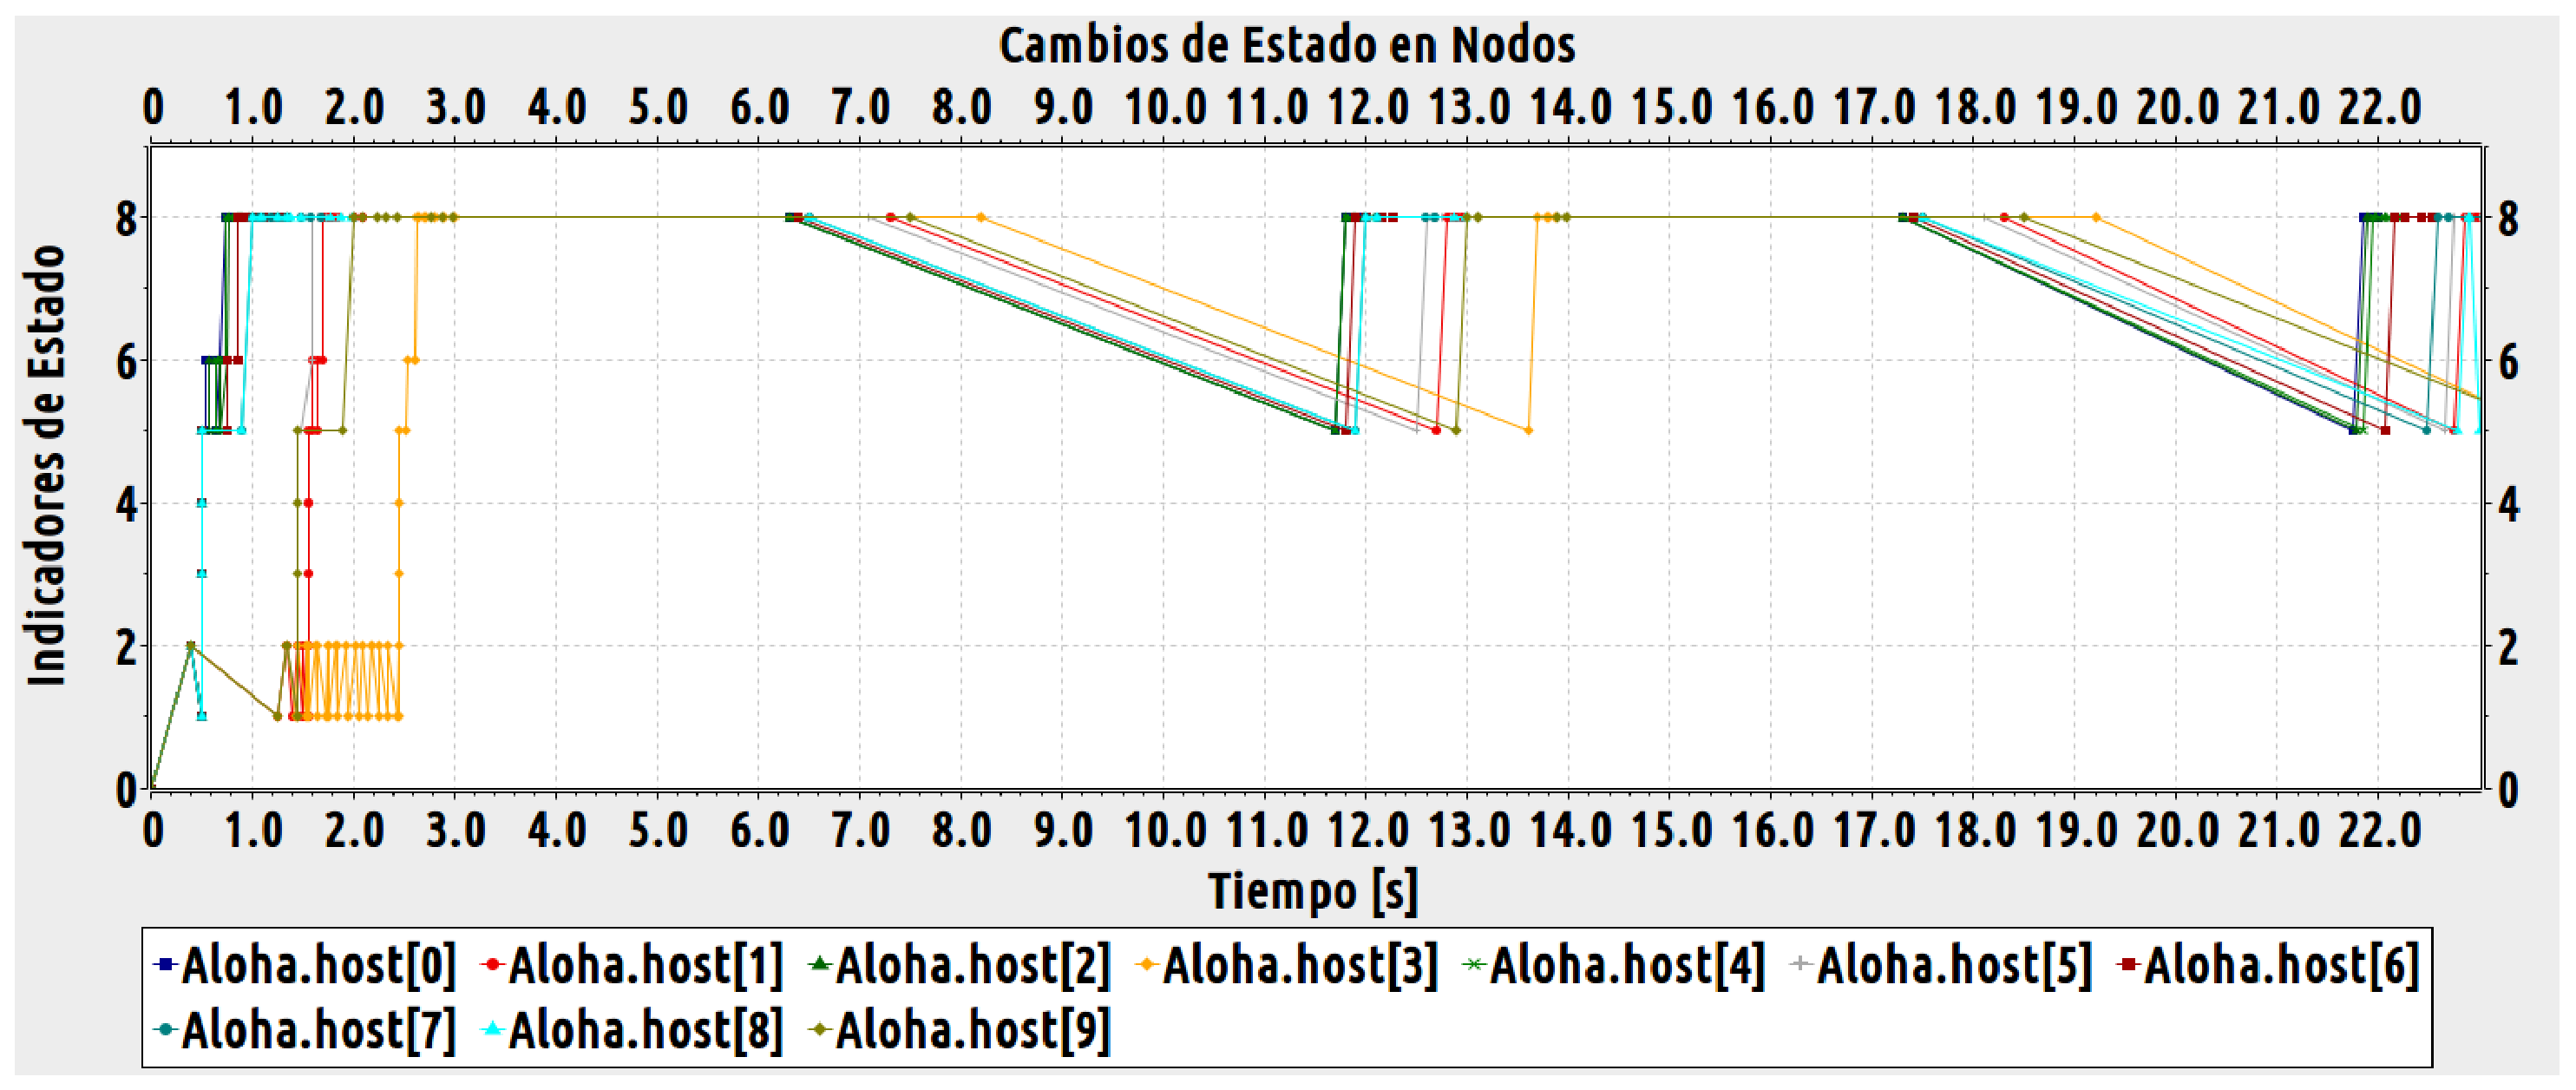
\includegraphics[angle=270, scale=0.4]{images/cambioestado10nodos.eps}
\caption{Gráfico de cambios de estados por tiempo en segundos, con diez nodos transmitiendo}
\label{anexa:2}
\end{figure}

\begin{figure}[!ht]
\centering
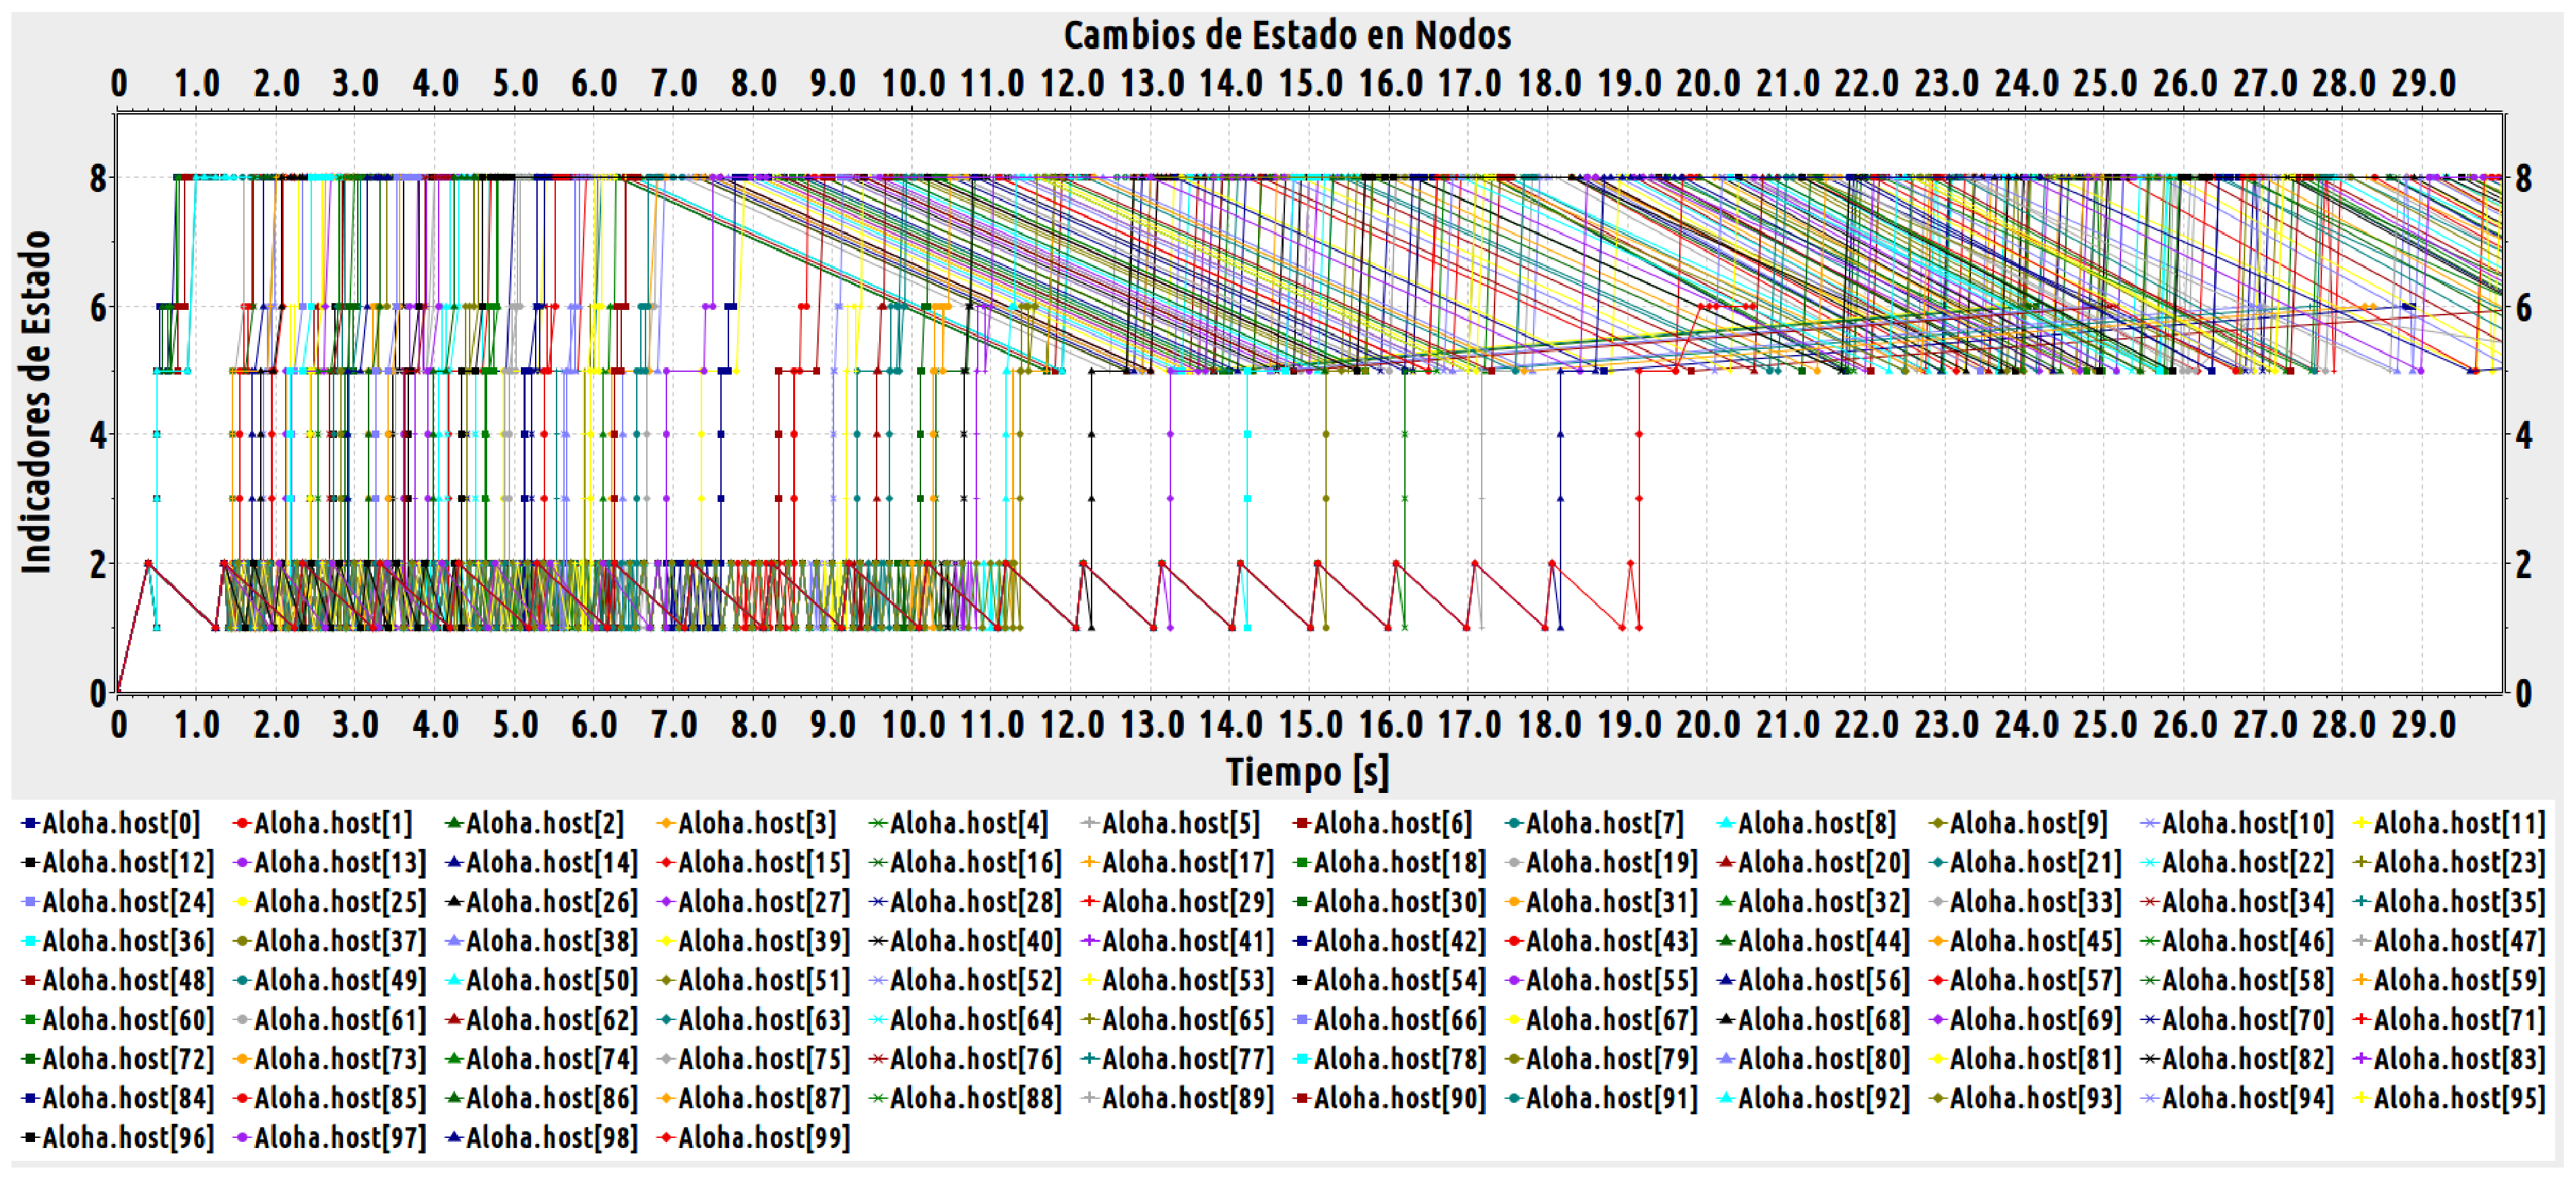
\includegraphics[angle=270, scale=0.3]{images/cambioestado100nodos.eps}
\caption{Gráfico de cambios de estados por tiempo en segundos, con cien nodos transmitiendo}
\label{anexa:3}
\end{figure}


%asd
\chapter{Anexo B}

%%pruebas con 5 nodos
\begin{figure}[!ht]
\centering
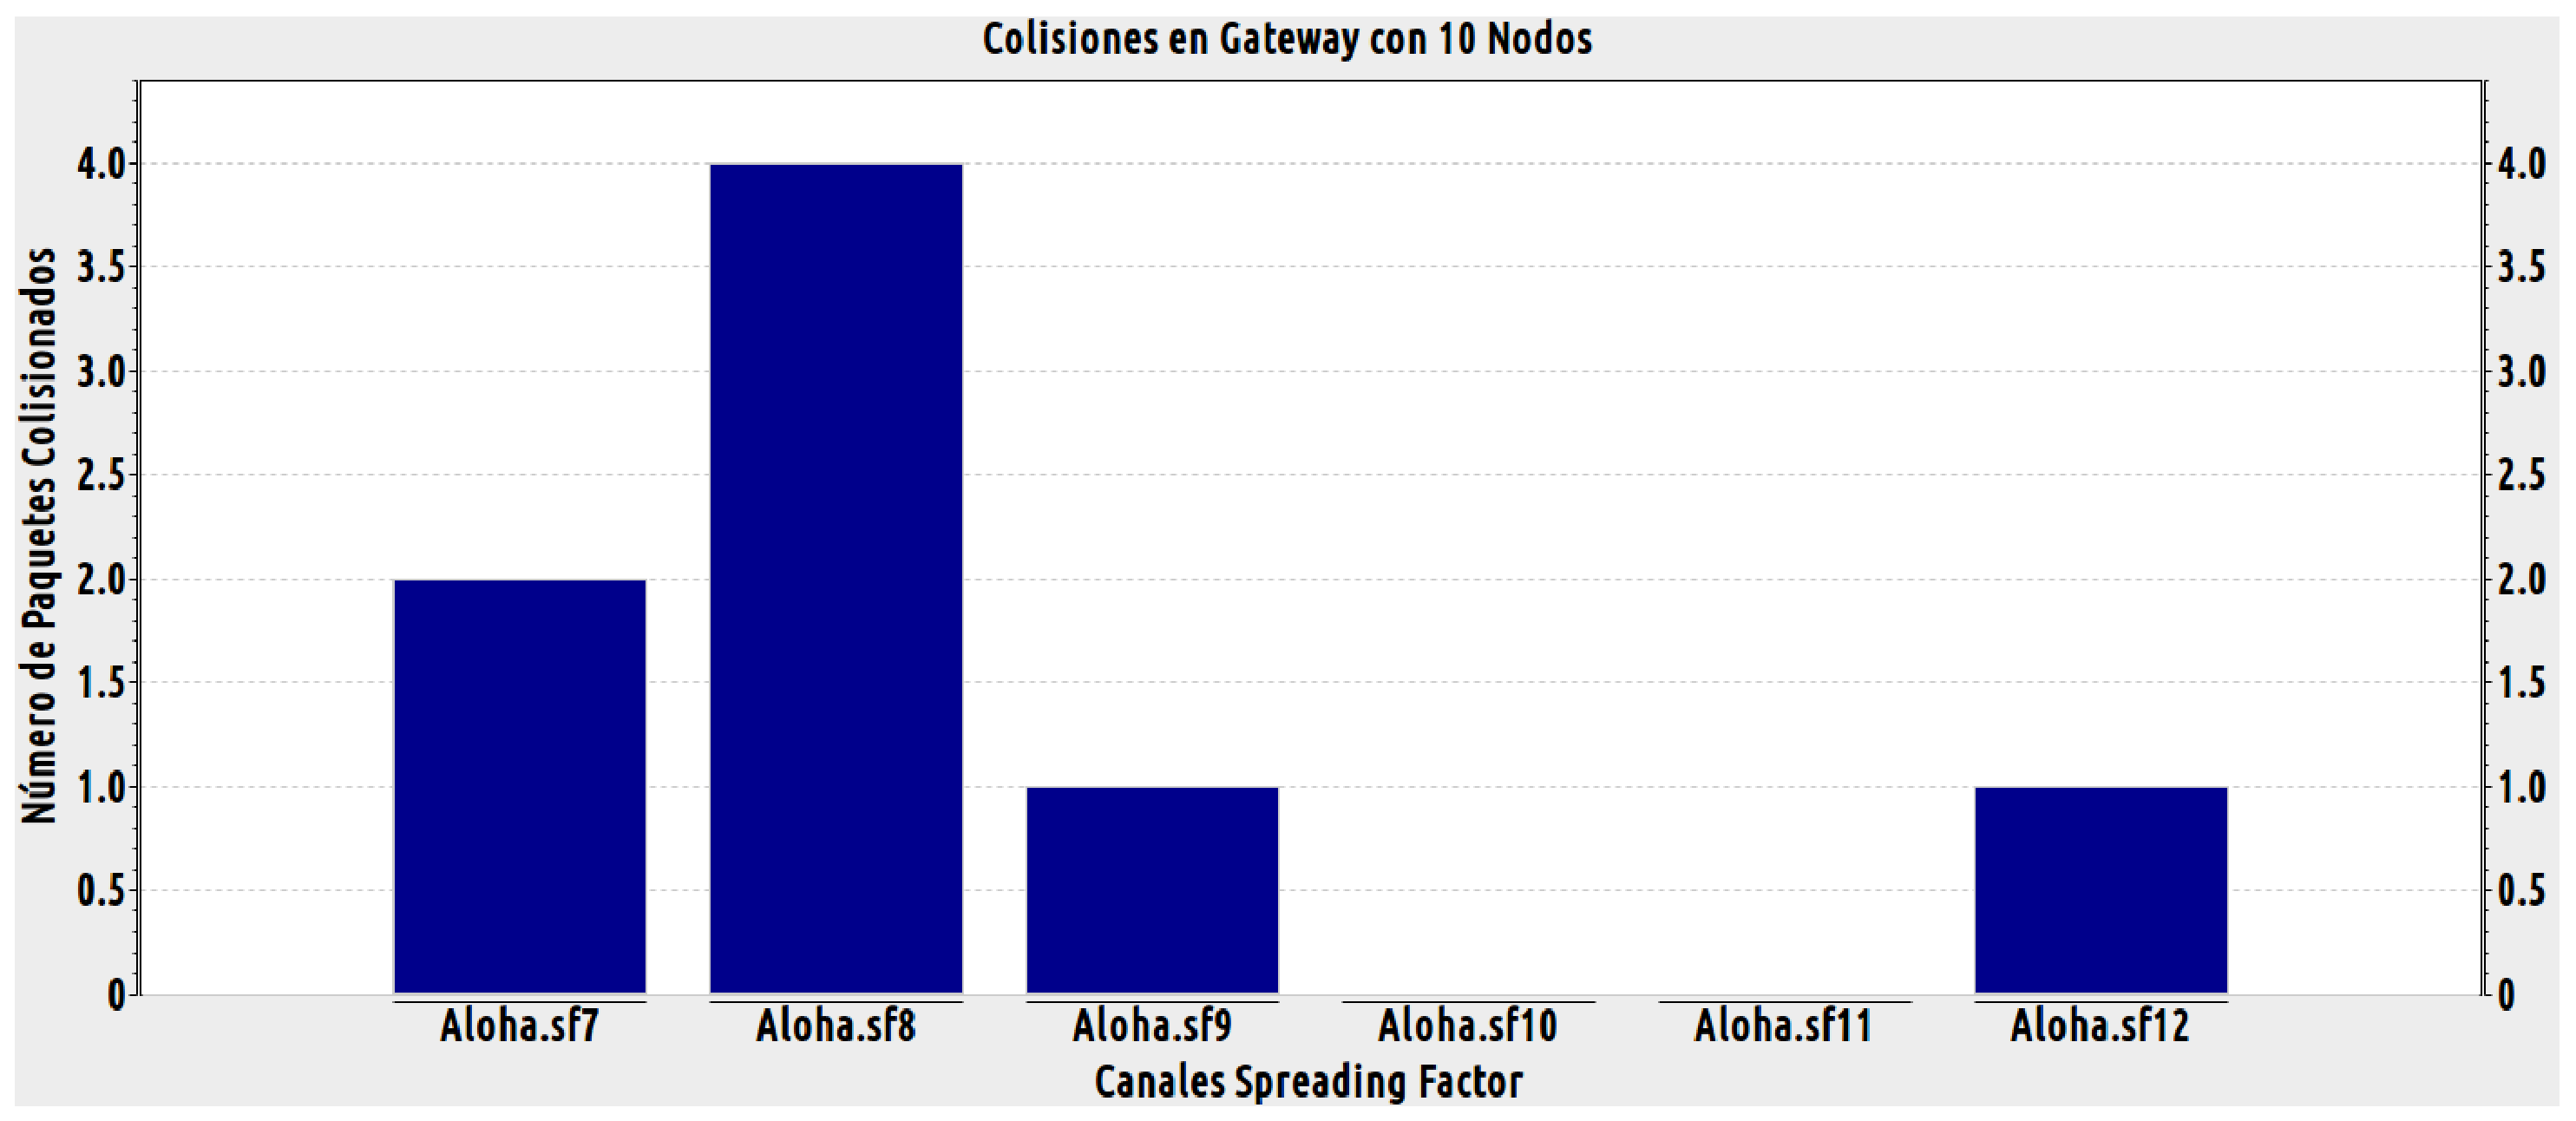
\includegraphics[angle=270, scale=0.4]{images/colisiones10nodos.eps}
\caption{Gráfico de colisiones ocurridos entre los distintos SF, para 10 nodos transmitiendo}
\label{anexb:1}
\end{figure}


\begin{figure}[!ht]
\centering
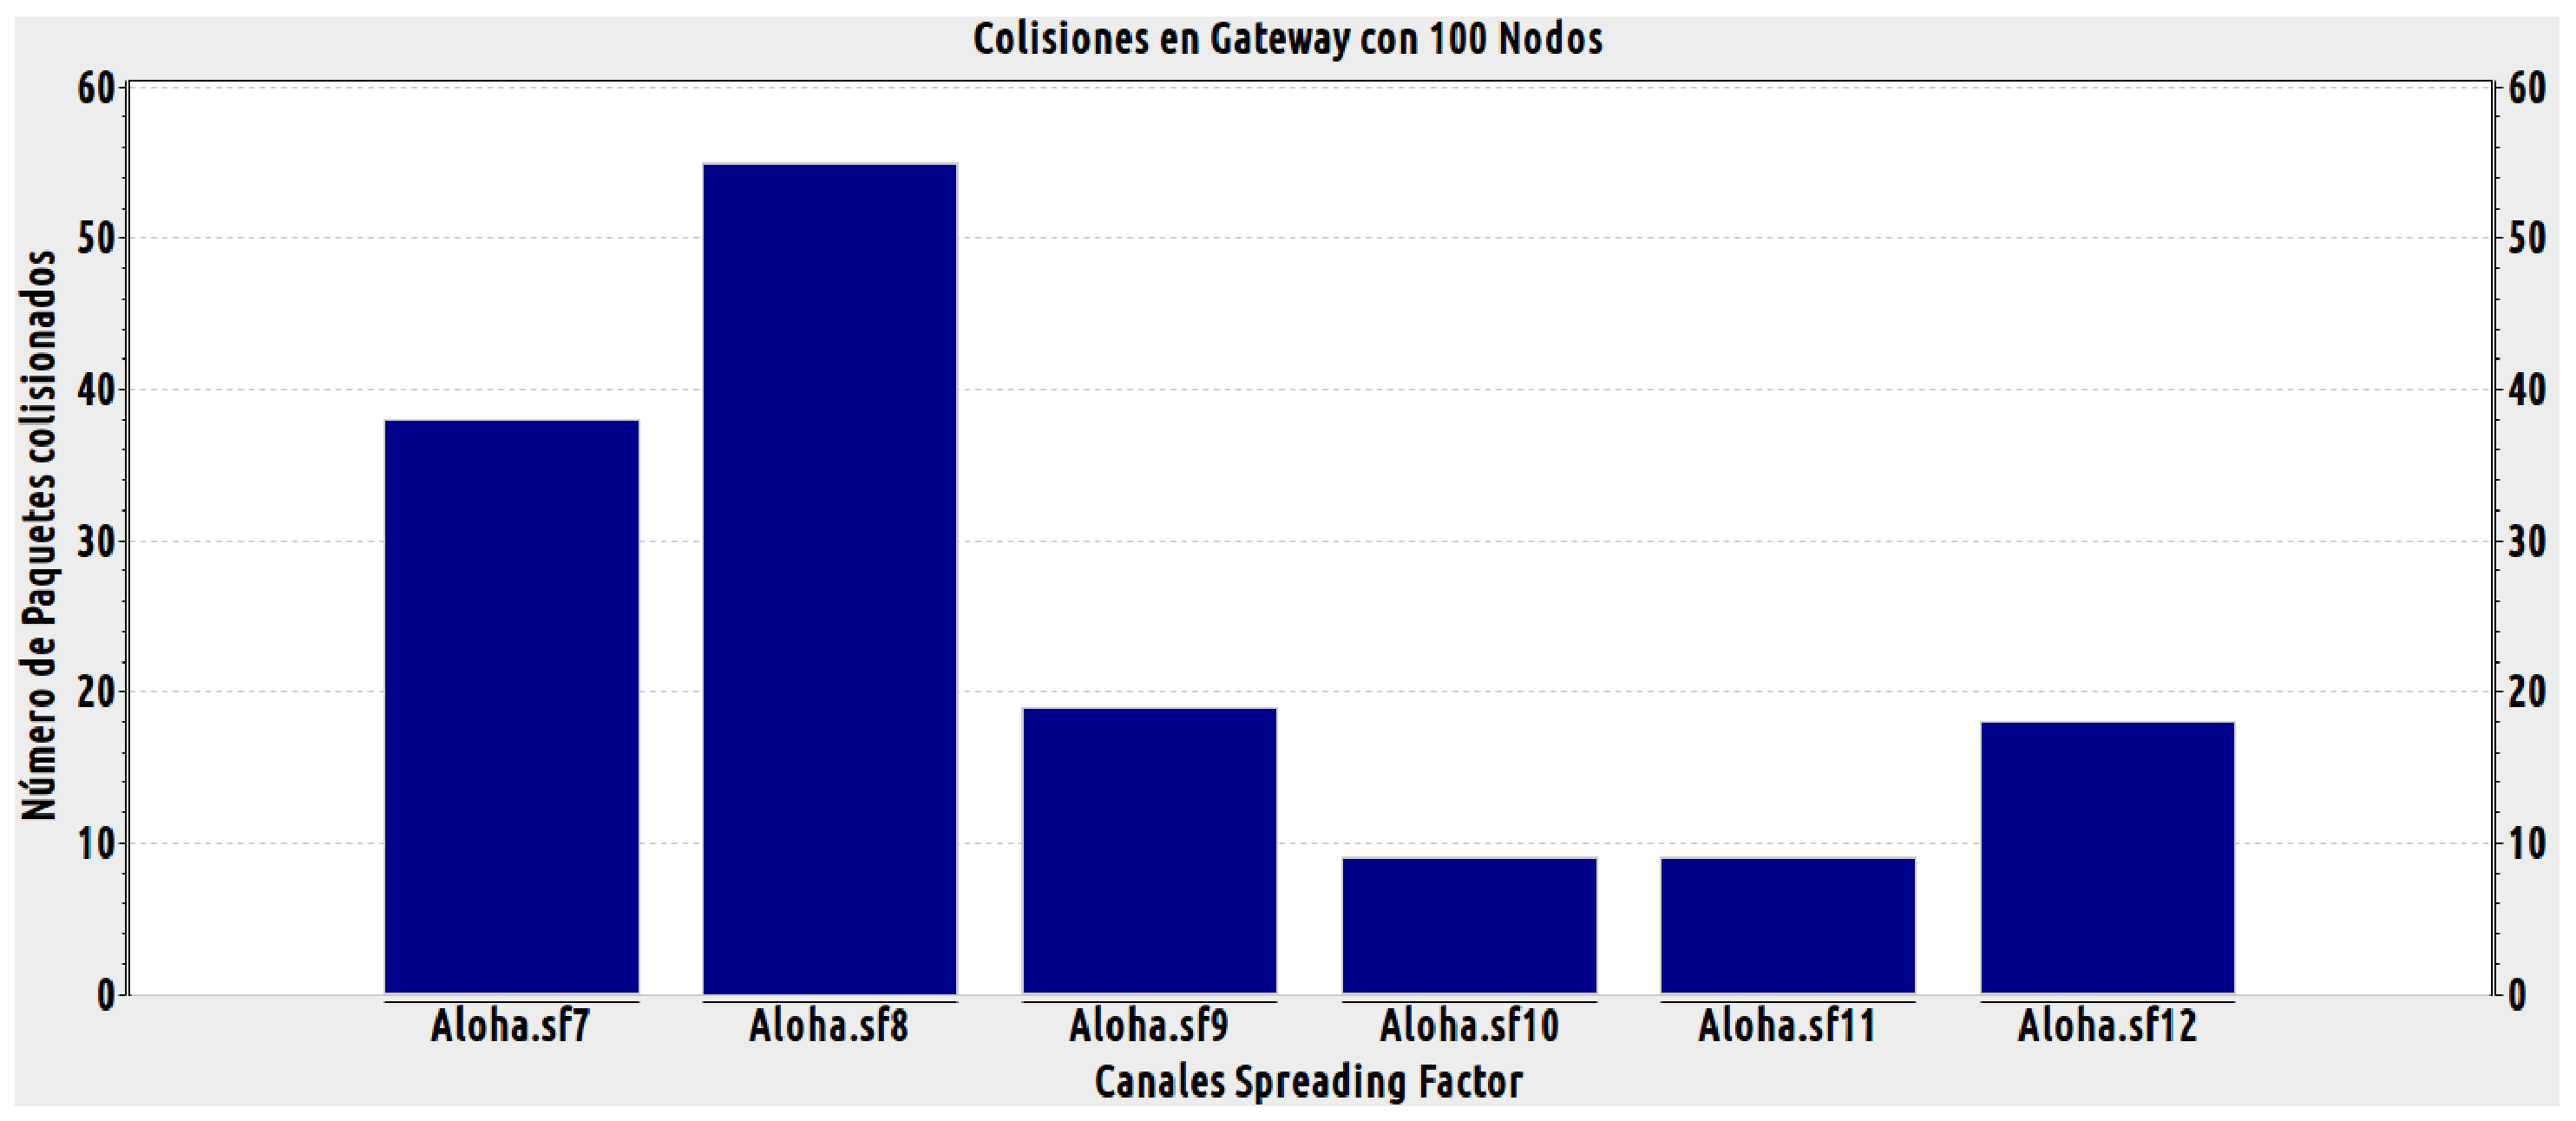
\includegraphics[angle=270, scale=0.4]{images/colisiones100nodos.eps}
\caption{Gráfico de colisiones ocurridos entre los distintos SF, para 100 nodos transmitiendo}
\label{anexb:2}
\end{figure}

%% pruebas con 50 nodos
\begin{figure}[!ht]
\centering
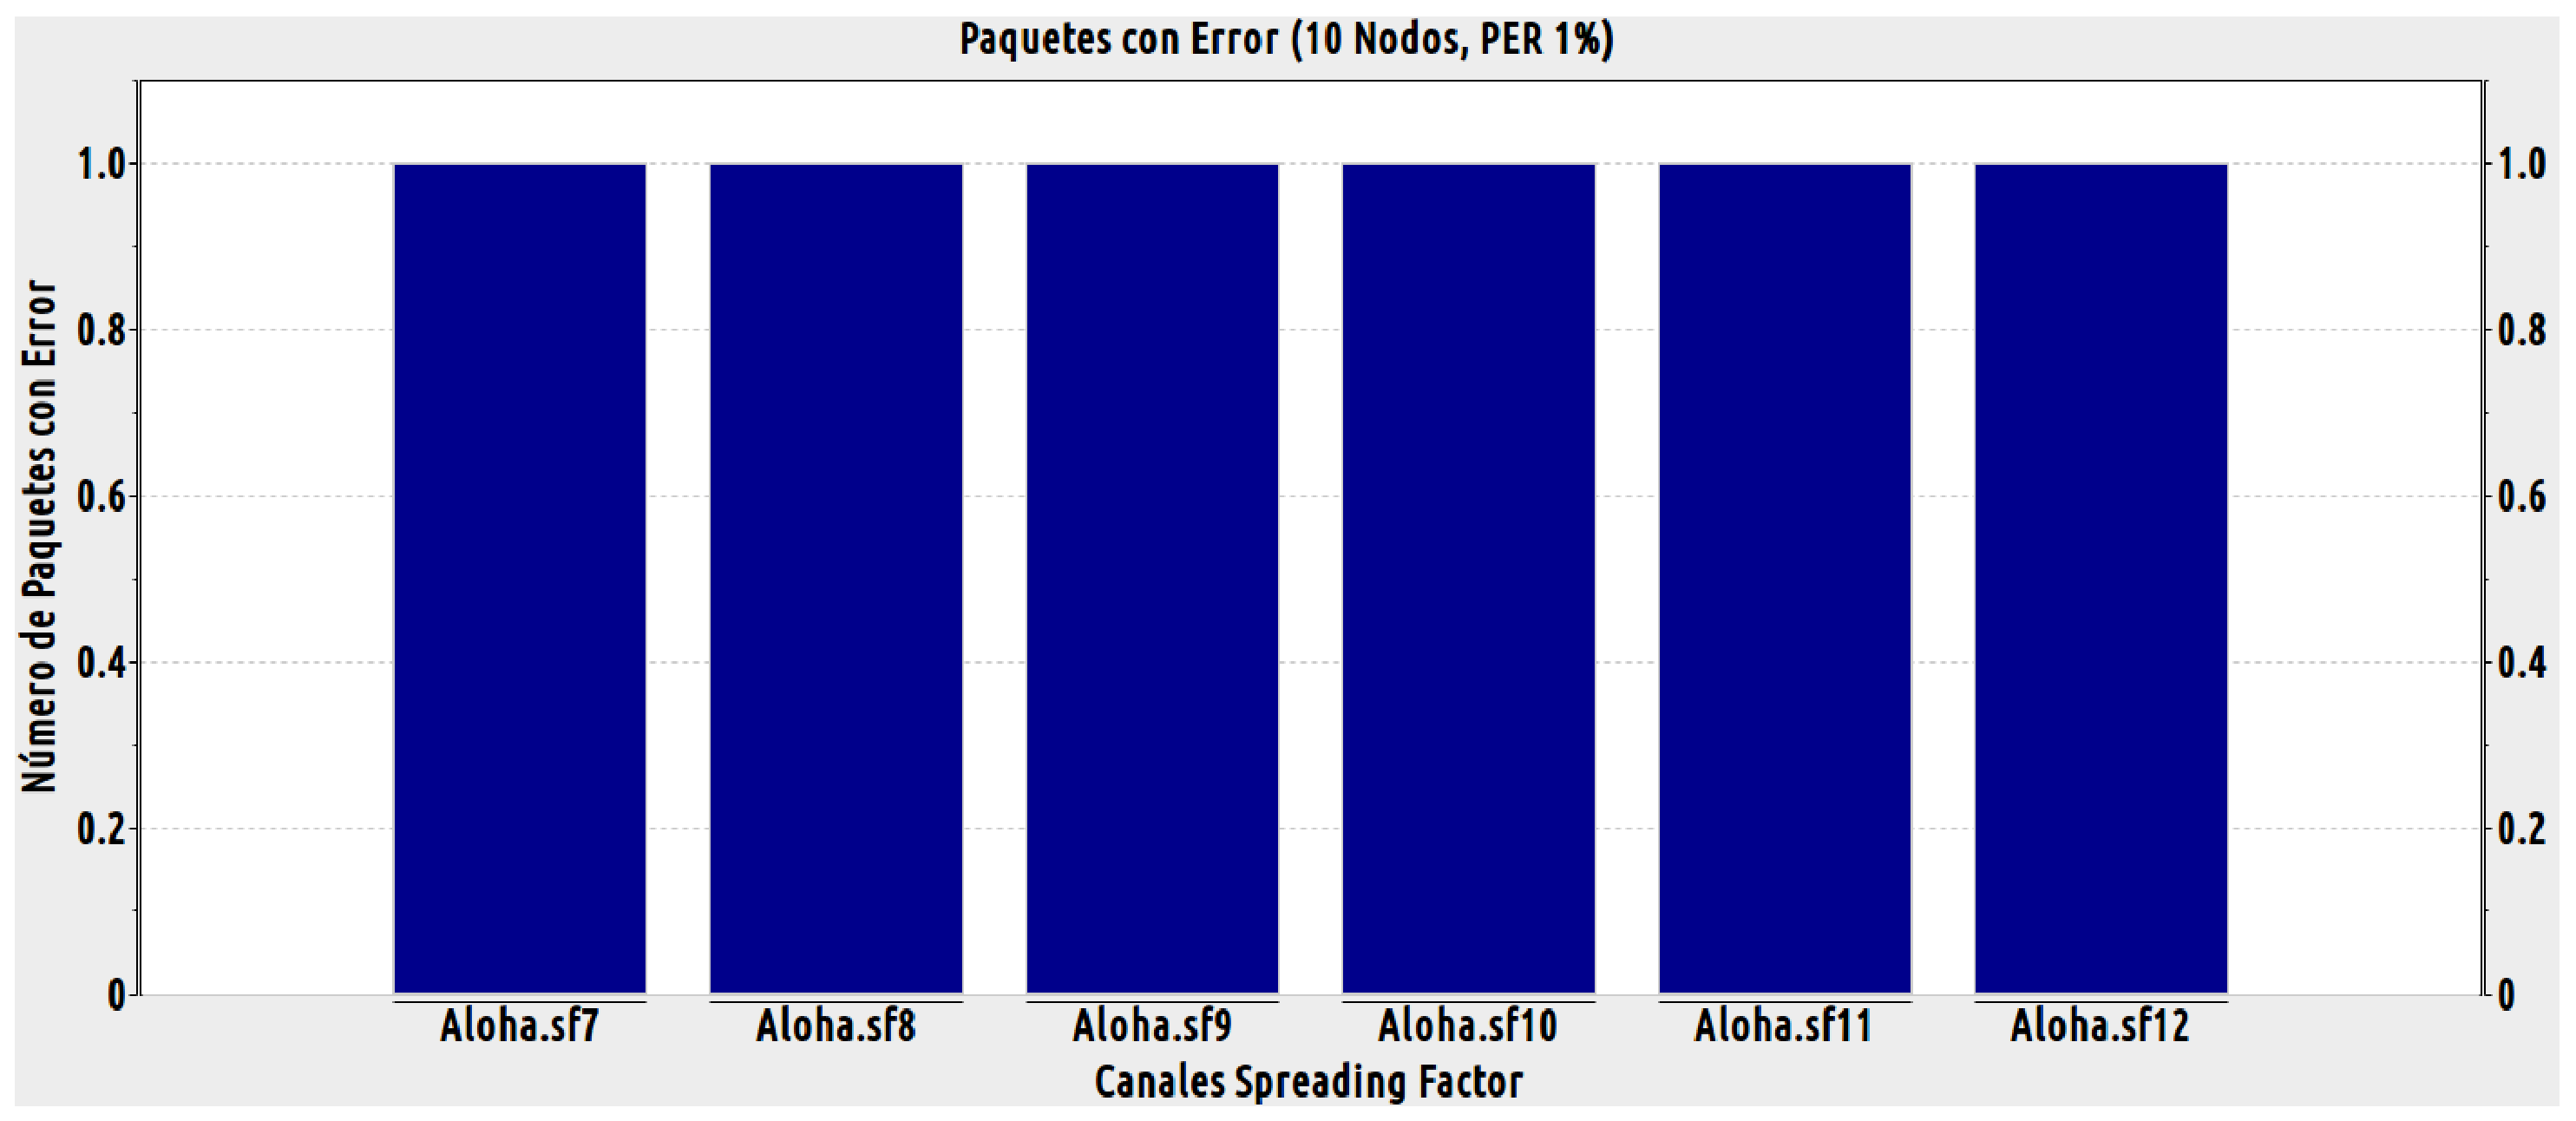
\includegraphics[angle=270, scale=0.4]{images/errores10nodos.eps}
\caption{Gráfico de cantidad de paquetes con errores en cada SF en la simulación, para 10 nodos}
\label{anexb:3}
\end{figure}

\begin{figure}[!ht]
\centering
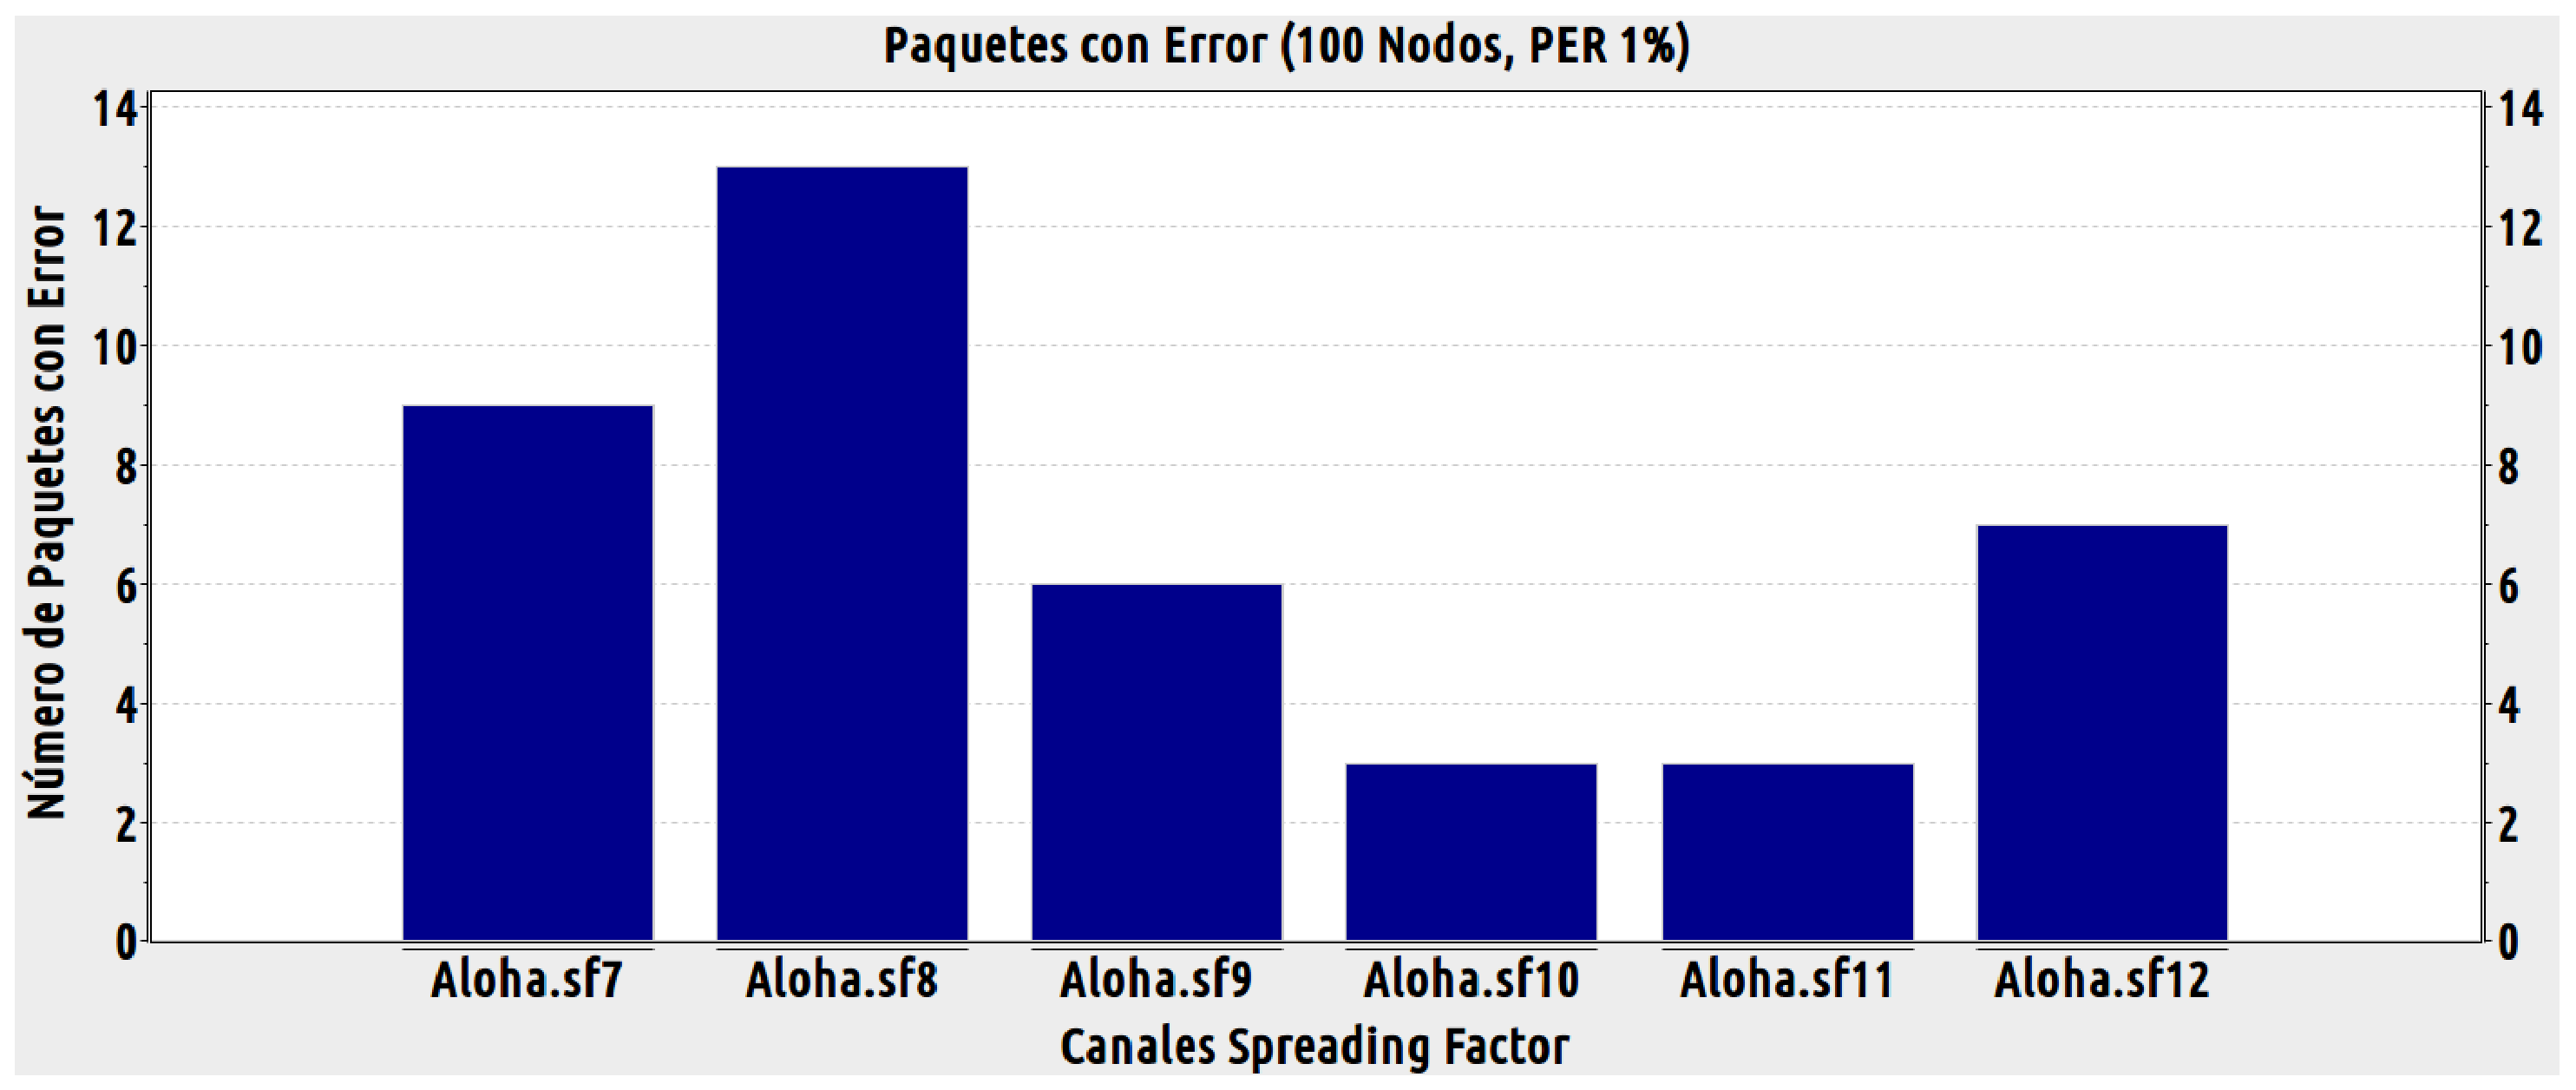
\includegraphics[angle=270, scale=0.4]{images/errores100nodos.eps}
\caption{Gráfico de cantidad de paquetes con errores en cada SF en la simulación, para 100 nodos}
\label{anexb:4}
\end{figure}

\chapter{Anexo C}
\lstset{language=C, 
showstringspaces=false,
backgroundcolor=\color{white},
breakatwhitespace=false,         % sets if automatic breaks should only happen at whitespace
  breaklines=true,                 % sets automatic line breaking
  captionpos=b,                    % sets the caption-position to bottom
  commentstyle=\color{mygreen},    % comment style
  deletekeywords={...},            % if you want to delete keywords from the given language
  escapeinside={\%*}{*)},          % if you want to add LaTeX within your code
  extendedchars=true,              % lets you use non-ASCII characters; for 8-bits encodings only, does not work with UTF-8
  frame=single,	                   % adds a frame around the code
  keepspaces=true,                 % keeps spaces in text, useful for keeping indentation of code (possibly needs columns=flexible)
  keywordstyle=\color{blue},       % keyword style
  language=Octave,                 % the language of the code
  morekeywords={*,...},           % if you want to add more keywords to the set
  numbers=left,                    % where to put the line-numbers; possible values are (none, left, right)
  numbersep=5pt,                   % how far the line-numbers are from the code
  numberstyle=\tiny\color{mygray}, % the style that is used for the line-numbers
  rulecolor=\color{black},         % if not set, the frame-color may be changed on line-breaks within not-black text (e.g. comments (green here))
  showspaces=false,                % show spaces everywhere adding particular underscores; it overrides 'showstringspaces'
  showstringspaces=false,          % underline spaces within strings only
  showtabs=false,                  % show tabs within strings adding particular underscores
  stepnumber=2,                    % the step between two line-numbers. If it's 1, each line will be numbered
  stringstyle=\color{mymauve},     % string literal style
  tabsize=2,	                   % sets default tabsize to 2 spaces
  title=\lstname  }
\begin{lstlisting}[frame=single,caption=Extracto de código del módulo de transición LoRa/IPv6	]  % Start your code-block
/* main loop */
    while (true) {
        /* fetch packets */
        if(tun_fd != -1){
         nread = read(tun_fd,buffer,sizeof(buffer));   
            RoHC_package = SCHC_TX(IPv6ToMesh(buffer,nread,lowpanh),(nread - 40) +27);
            //RoHC_package = IPv6ToMesh(buffer,nread,lowpanh);
            if(RoHC_package != NULL){
                printf("%s\n","manda mensaje");
                txpkt.size = (nread - 40) + 3;
                //txpkt.size = (nread - 40) + 27;
                for(j = 0; j < txpkt.size; j++ ){
                    txpkt.payload[j] = RoHC_package[j];
                    printf("%i-", RoHC_package[j]);}
                printf("\n");
                i = lgw_send(txpkt);

                wait_ms(delay);
        //wait_ms(1);
                nb_pkt = lgw_receive(ARRAY_SIZE(rxpkt), rxpkt);
                /* log packets */
                if(nb_pkt > 0){
                    printf("%s\n","LLega mensaje");
                    p = &rxpkt[0];
                    for(i = 0; i < p->size; i++){
                        printf("%i-", p->payload[i]);}
                    //Inicio de socket para enviar a bdd datos de LoRa//
                    printf("\n");
//Inicio de socket para enviar a bdd datos de LoRa//
MYSQL *con = mysql_init(NULL);
if (con == NULL){
	fprintf(stderr, "%s\n", mysql_error(con));
    exit(1);}
if (mysql_real_connect(con,"fe80::8dfe:9b57:3ea6:dbed","tesis", "tesis","testdb", 0, NULL, 0) == NULL){
	finish_with_error(con);} 
struct ifaddrs *ifaddr, *ifa;
int family, s;
char host[NI_MAXHOST];
if (getifaddrs(&ifaddr) == -1){
	perror("getifaddrs");
	exit(EXIT_FAILURE);}
for (ifa = ifaddr; ifa != NULL; ifa = ifa->ifa_next){
	if (ifa->ifa_addr == NULL)
		continue;  
	s=getnameinfo(ifa->ifa_addr,
	sizeof(struct sockaddr_in),host, NI_MAXHOST,
	 NULL, 0, NI_NUMERICHOST);
	if((strcmp(ifa->ifa_name,"eth0")==0)&&
	(ifa->ifa_addr->sa_family==AF_INET)){
    	 if (s != 0){
       	 	printf("getnameinfo() failed: 
       	 	%s\n", gai_strerror(s));
        	exit(EXIT_FAILURE);}
         printf("\tInterface:<%s>\n",ifa->ifa_name);
         printf("\t  Address:<%s>\n", host);}}
freeifaddrs(ifaddr);
	/*Insercion de ip de GW que envia datos,
	 y payload obtenido desde el nodo*/
	if (mysql_query(con,
	"INSERT INTO tesis VALUES(host, p->paylod)")){
		finish_with_error(con);
	}
    /*Impresion por pantalla 
    de datos en la tabla tesis */  
	if (mysql_query(con, "SELECT * FROM tesis")){
    	finish_with_error(con);
  	} 
	MYSQL_RES *result = mysql_store_result(con);
	if (result == NULL){
		finish_with_error(con);
	}
	int num_fields = mysql_num_fields(result);
    MYSQL_ROW row;
    while ((row = mysql_fetch_row(result))){ 
	for(int i = 0; i < num_fields; i++){ 
		printf("%s ", row[i] ? row[i] : "NULL"); 
		} 
	}
	 mysql_free_result(result);
	 mysql_close(con);// Termino de uso de Socks//
\end{lstlisting}
\label{anexc:1}

%\lstinputlisting[caption="Módulo de transición desde LoRa a IPv6"]{}
%\lstinputlisting[language=C, firstline=512, lastline=600]{/home/w01f/Documents/respaldo-raspberry/home/pi/lora/project_ipv6/src/project_ipv6.c}
% puede incluir más archivos de anexos
% \input{anexo-dos}
\end{document}
% that's all folks